\documentclass[11pt,letterpaper]{article}
\usepackage[margin=1in]{geometry}
\usepackage[T1]{fontenc}
\usepackage{lmodern,microtype,amsmath,amssymb,amsthm,mathtools}
\usepackage{booktabs,array,enumitem,xcolor}
\usepackage{tikz}
\usetikzlibrary{positioning,arrows.meta,calc,decorations.pathreplacing}
\tikzset{
  stage/.style={draw,rounded corners=2.5pt,align=left,
    inner xsep=8pt,inner ysep=5pt,text width=0.74\textwidth},
  flow/.style={-{Stealth[length=2.6mm]},semithick},
  gapbrace/.style={decorate,decoration={brace,amplitude=4pt}},
}
\usepackage[colorlinks=true,linkcolor=blue!45!black,citecolor=blue!45!black,urlcolor=blue!45!black]{hyperref}
\usepackage[nameinlink,noabbrev]{cleveref}
\setlength{\parindent}{1.2em}
\setlength{\parskip}{0pt}
\setlist{itemsep=2pt,topsep=4pt}
\allowdisplaybreaks[2]
\newtheorem{theorem}{Theorem}[section]
\newtheorem{lemma}[theorem]{Lemma}
\newtheorem{proposition}[theorem]{Proposition}
\newtheorem{corollary}[theorem]{Corollary}
\newtheorem{claim}[theorem]{Claim}
\newtheorem{fact}[theorem]{Fact}
\theoremstyle{definition}
\newtheorem{definition}[theorem]{Definition}
\newtheorem{assumption}[theorem]{Imported interface}
\theoremstyle{remark}
\newtheorem{remark}[theorem]{Remark}
\newcommand{\E}{\mathbb E}
\newcommand{\F}{\mathbb F}
\newcommand{\R}{\mathbb R}
\newcommand{\N}{\mathbb N}
\newcommand{\Z}{\mathbb Z}
\newcommand{\THR}{\mathrm{THR}}
\newcommand{\SYM}{\mathrm{SYM}}
\newcommand{\ENP}{\mathrm{E}^{\mathrm{NP}}}
\newcommand{\poly}{\operatorname{poly}}
\newcommand{\polylog}{\operatorname{polylog}}
\newcommand{\ind}{\mathbf 1}
\newcommand{\supp}{\operatorname{supp}}
\newcommand{\Inf}{\operatorname{Inf}}
\newcommand{\tr}{\operatorname{tr}}
\newcommand{\diag}{\operatorname{diag}}
\newcommand{\rank}{\operatorname{rank}}
\newcommand{\Enc}{\operatorname{Enc}}
\newcommand{\Cons}{\operatorname{Cons}}
\newcommand{\sgn}{\operatorname{sgn}}
\newcommand{\agr}{\operatorname{agr}}
\newcommand{\ceil}[1]{\left\lceil #1\right\rceil}
\newcommand{\floor}[1]{\left\lfloor #1\right\rfloor}
\newcommand{\abs}[1]{\left|#1\right|}
\newcommand{\norm}[1]{\left\|#1\right\|}
\newcommand{\ip}[2]{\left\langle #1,#2\right\rangle}
\newcommand{\eps}{\varepsilon}
\newcommand{\eqdef}{\mathrel{:=}}
\newcommand{\capp}{\mathrm{CAPP}}
% This is the named canonical preprint. Prepare an anonymous copy separately
% if the destination conference requires double-blind submission.
\title{Wire--Correlation Tradeoffs at Exponent $7/2$\texorpdfstring{\\}{: }for Depth-Two Threshold Circuits}
\author{Dev Nag\\
CtrlStack, Inc.\\
\texttt{devnag@gmail.com}\\
\href{https://orcid.org/0009-0006-7304-8082}{\nolinkurl{https://orcid.org/0009-0006-7304-8082}}}
\date{Version 1: September 15, 2026}

\begin{document}
\hypersetup{pageanchor=false}
\begin{titlepage}
\maketitle
\thispagestyle{empty}
\begin{abstract}
We prove almost-everywhere correlation lower bounds for unrestricted
$\THR\circ\THR$ and $\SYM\circ\THR$ circuits measured by physical
wires, raising the wire-exponent frontier for these classes from $3$
to $7/2$, up to logarithmic factors. Write
$L=\lceil\log_2(n+2)\rceil$. For every fixed $c>0$ and $K_T>5+2c$,
$K_S>4+2c$, there is one language in $\ENP$, depending on $c,K_T,K_S$
but on nothing else, such that for every fixed pair of multipliers
$A_T,A_S>0$ and every sufficiently large $n$: every $\THR\circ\THR$
circuit with at most $A_T\,n^{7/2}/L^{K_T}$ wires, and every
$\SYM\circ\THR$ circuit with at most $A_S\,n^{7/2}/L^{K_S}$ wires,
agrees with the language on less than a $1/2+L^{-c}$ fraction of
inputs. Further regimes trade the denominator against the advantage:
endpoint powers $L^5,L^4$ at constant advantage with suitably small
positive coefficients, a $\log^*n$ variant, and polynomial advantage
$n^{-c}$ at caps $n^{7/2-\varepsilon}$ for every fixed
$0<c<\varepsilon/2$, the range $\varepsilon>1/2$ following from the
author's earlier near-cubic wire theorem~\cite{NagCubic}. Since a
normalized circuit with $G$ bottom-gate occurrences has at most
$(n+1)G$ wires, gate-small circuits are wire-small, and the
constant-advantage endpoint gives almost-everywhere correlation gate
bounds at positive-coefficient caps $n^{5/2}/L^{5}$ and
$n^{5/2}/L^{4}$, improving the author's earlier gate preprint in both
the logarithmic denominators and the form of hardness.

Two ideas drive the improvement. First, building on the
restriction-and-CAPP framework of Chen, Tal, and Wang, coordinate
restrictions are replaced by a partition of the cube into products of
Hamming-code stars: the partition charges a threshold only for
genuinely mixed dependence on the two live halves of a
cell---one-sided behavior, however complicated, is absorbed into
exact scores---and the mixed difference is nonzero with probability
$O(r^{3/2}f/n^{3/2})$ for fan-in $f$ and $r$ blocks. Second, that
structural gain must survive two hostile conversions---deterministic
counting and hardness amplification---and most of the new machinery
exists to keep each conversion from spending it. A matrix sampler
with one fixed trace moment is accurate for all rank-one selectors
simultaneously, so the absorbed one-sided behavior never has to be
enumerated; repaired count lists keep every reported count state
Boolean, with controlled intermediate ranges, even on failed hash
seeds; and a sparse masked verifier carries the counting algorithm
through the Chen--Lyu--Williams almost-everywhere transfer without
multiplying discarded mass by the coefficient mass of an XOR
reconstruction. We specify the imported algorithm-to-lower-bound
interfaces, prove the new compiler and transfer steps in detail, and
give three scoped obstructions to stronger conclusions from these
methods.
\end{abstract}
\end{titlepage}
\setcounter{page}{1}
\hypersetup{pageanchor=true}
{\small\setcounter{tocdepth}{1}\tableofcontents}
\clearpage

\section{Results and scope}
\label{sec:results}

A linear threshold gate computes a Boolean halfspace with arbitrary
real weights. The depth-two classes $\THR\circ\THR$ and
$\SYM\circ\THR$ are among the simplest circuit models for which
superpolynomial lower bounds remain open, and progress on them has
historically required new circuit-analysis algorithms. Kane and
Williams~\cite{KaneWilliams} proved $\widetilde\Omega(n^{5/2})$-wire
average-case hardness for an explicit function; Chen, Tal, and
Wang~\cite{CTW} reached worst-case gate caps $n^{5/2-\varepsilon}$
for $\ENP$; the author's near-cubic manuscript~\cite{NagCubic} gave
almost-everywhere correlation hardness at wire caps $n^3/\polylog n$.
This paper raises the wire exponent to $7/2$.

\begin{center}
\small
\begin{tabular}{@{}llll@{}}
\toprule
 & Resource scale & Hardness type & Hard function\\
\midrule
Kane--Williams~\cite{KaneWilliams} & $\widetilde\Omega(n^{5/2})$ wires & average-case & explicit, linear time\\
Chen--Tal--Wang~\cite{CTW} & $n^{5/2-\varepsilon}$ gates & worst-case & $\ENP$\\
Near-cubic~\cite{NagCubic} & $n^{3}/\polylog n$ wires & a.e.\ correlation & $\ENP$\\
This paper & $n^{7/2}/\polylog n$ wires & a.e.\ correlation & $\ENP$\\
\bottomrule
\end{tabular}
\end{center}

The two correlation entries occupy different advantage regimes: the
near-cubic bound forbids every fixed inverse-polynomial advantage at
its caps, while the parameterized $7/2$-scale theorem gives
inverse-polylogarithmic advantage. Rows A and C of \cref{tab:regimes}
trade advantage for smaller denominators, and row D gives
inverse-polynomial advantage at wire caps $n^{7/2-\varepsilon}$.
The advance is a tradeoff curve, not an across-the-board replacement
of the earlier result.

The source of the new exponent can be shown in one schematic
calculation. The algorithm partitions the cube into cells with
$2^{k/2}\times2^{k/2}$ live points; a bottom threshold contributes to
the genuinely \emph{mixed} part of a cell---dependence on both live
halves jointly---with probability $O(r^{3/2}f/q^{3/2})$ in its fan-in
$f$, so a circuit with $W$ wires has mean mixed-residual population
$O(W/q^{3/2})$, suppressing logarithmic factors and averaging over
complete inputs. A budget $B$ at this scale suffices: sparsity filters
suppress populations above $CB$, for a fixed $C>1$, with
inverse-polynomial error, and enlarged-cap lists cover the transition
region. The counting compiler pays roughly $\sqrt B$, and that cost
must fit inside the compiler's linear-in-$q$ load allowance. The
largest affordable cap is therefore
\[
\sqrt{W/q^{3/2}}\lesssim q
\qquad\Longleftrightarrow\qquad
W\lesssim q^{7/2}.
\]
Here $q$ is the algorithm's native input length; the final language
length $n$ is a regime-dependent dilation of $q$, at most logarithmic,
and the distinction between the two scales is maintained throughout.
Everything else in the paper is the price of
making this schematic exact: logarithmic compilation costs, the
reconstruction mass of the hardness transfer, and the length changes
of XOR amplification produce the denominators and quantifiers below.

One design principle runs through every stage: \emph{never pay for
what can be absorbed exactly}. The partition absorbs arbitrary
one-sided behavior into exact scores and charges only left--right
coincidences. The compiler converts products to parities, paying
integer precision rather than Boolean degree. One fixed sampler
serves every selector, paying a dimension factor in samples rather
than a union bound in error. The transfer charges masked losses once,
against a bounded honest value, rather than multiplying them by the
mass of a polynomial expansion. Each later section names its instance
of this principle.

The results form a family: the exponent $7/2$ is common to all of
them, while three parameters trade against one another---the
logarithmic denominator, the allowed agreement, and the quantifier on
the leading coefficient. We state the parameterized tradeoff first
and then its named regimes.

Let $L(n)=\lceil\log_2(n+2)\rceil$ and
$v(n)=\max\{2,\log_2^*n\}$. A threshold gate outputs
$\ind[\sum_i a_i x_i\ge\theta]$, with arbitrary real weights in the
lower-bound statements. A symmetric gate applies an arbitrary Boolean
function to the number of its input ones. A circuit is strictly layered:
inputs feed threshold gates, which feed one threshold or symmetric gate.
We count bottom-gate occurrences and all input-to-bottom and bottom-to-top
incidences. Parallel input incidences can be combined before applying an
algorithm; retaining them only increases the charged wire count.
For Boolean functions on $n$ bits put
$\agr(F_n,C)=\Pr_{x\in\{0,1\}^n}[F_n(x)=C(x)]$.
Almost everywhere means at every sufficiently large integer length.
The class $\ENP$ is deterministic $2^{O(n)}$ time with an NP oracle,
the standard home of hard functions in the algorithm-to-lower-bound
framework: the language is explicitly computable there, though not
efficiently.

\begin{theorem}[Parameterized wire--correlation tradeoff]
\label{thm:tradeoff}
Fix $c>0$ and real constants $K_T>5+2c$ and $K_S>4+2c$.
There is a language $F\in\ENP$ such that, for every pair of fixed
constants $A_T,A_S>0$, there is $n_0$ for which, for every $n\ge n_0$,
\begin{align*}
W(C)\le A_T n^{7/2}/L(n)^{K_T},\quad C\in\THR\circ\THR
&\quad\Longrightarrow\quad \agr(F_n,C)<\tfrac12+L(n)^{-c},\\
W(C)\le A_S n^{7/2}/L(n)^{K_S},\quad C\in\SYM\circ\THR
&\quad\Longrightarrow\quad \agr(F_n,C)<\tfrac12+L(n)^{-c}.
\end{align*}
The language may depend on $c,K_T,K_S$, but not on $A_T,A_S$;
the onset $n_0$ may depend on the multipliers.
\end{theorem}

This order of quantifiers is part of the theorem. In particular, the
notation $O(\cdot)$ in an informal summary must not suggest that a
different language is chosen for each hidden constant. The strict
inequalities on $K_T,K_S$ provide the slack that absorbs every fixed
multiplier and the change of input length in XOR amplification.

Table~\ref{tab:regimes} gives representative regimes. The two entries in
each cap column refer, in order, to $\THR\circ\THR$ and
$\SYM\circ\THR$. The advantage is the additive term above $1/2$ in
the forbidden agreement. The table describes a family of achieved
tradeoffs, not an optimality theorem.

\begin{table}[ht]
\centering
\begin{tabular}{@{}c p{.31\textwidth} p{.33\textwidth} p{.18\textwidth}@{}}
\toprule
 & Wire caps, THR / SYM & Coefficient quantifier & Advantage\\
\midrule
A & $a_T n^{7/2}/L^5$, $a_S n^{7/2}/L^4$
  & Some positive coefficients, chosen after the required saving
  & Fixed $\gamma>0$\\[3pt]
B & $A_T n^{7/2}/L^{11/2}$, $A_S n^{7/2}/L^{9/2}$
  & Every fixed $A_T,A_S>0$ & $L^{-1/8}$\\[3pt]
C & $A_T n^{7/2}/(L^5v)$, $A_S n^{7/2}/(L^4v)$
  & Every fixed $A_T,A_S>0$ & $v^{-1/16}$\\[3pt]
D & $A_T n^{7/2-\varepsilon}$, $A_S n^{7/2-\varepsilon}$
  & Every fixed $A_T,A_S>0$ & $n^{-c}$, $0<c<\varepsilon/2$\\
\bottomrule
\end{tabular}
\caption{Named regimes of the wire--correlation tradeoff. All guarantees
are almost everywhere, with one common language for the two classes
within each fixed regime. Different regimes need not use the same language.
Row D is proved here for $0<\varepsilon\le1/2$
(\cref{thm:poly}); the extension to $\varepsilon>1/2$ is a consequence
of the earlier near-cubic theorem (\cref{cor:poly-prior}).}
\label{tab:regimes}
\end{table}

\begin{theorem}[Constant-advantage endpoint]
\label{thm:endpoint}
For every fixed $0<\gamma<1/2$ there are $a_T,a_S>0$ and a common
$F_\gamma\in\ENP$ such that, almost everywhere, the caps in row A
imply agreement less than $1/2+\gamma$. The constants are selected after
the fixed polynomial saving needed by the lower-bound transfer.
This statement does not assert every prescribed multiplier at the exact
powers $5$ and $4$.
\end{theorem}

\begin{theorem}[Slowly varying advantage]
\label{thm:slow}
There is a common $F\in\ENP$ such that, for every fixed $A_T,A_S>0$,
the caps in row C imply agreement less than $1/2+v(n)^{-1/16}$ almost
everywhere. The language is independent of the multipliers.
\end{theorem}

\begin{theorem}[Polynomial advantage in the native range]
\label{thm:poly}
For every fixed $0<\varepsilon\le1/2$ and $0<c<\varepsilon/2$, there is a
common $F\in\ENP$ such that, for every fixed $A_T,A_S>0$, the caps
in row D imply agreement less than $1/2+n^{-c}$ almost everywhere.
The language may depend on $\varepsilon,c$, but not on the multipliers.
\end{theorem}

\begin{corollary}[Polynomial-advantage extension from the near-cubic theorem]
\label{cor:poly-prior}
As a consequence of \cite[Theorem~2.3]{NagCubic}, for every fixed
$\varepsilon>1/2$ and $0<c<\varepsilon/2$, there is a common
$F\in\ENP$ such that, for every fixed $A_T,A_S>0$, the caps in row D
imply agreement less than $1/2+n^{-c}$ almost everywhere.
The language may depend on $\varepsilon,c$, but not on the multipliers.
\end{corollary}

The extension in \cref{cor:poly-prior} uses the earlier near-cubic
lower-bound theorem, not a stronger parameter range of the new supplier.
Its size comparison is given separately in Appendix~\ref{tr:appendix}.

\begin{corollary}[Gate consequences]
\label{cor:gates}
A circuit with $G$ bottom-gate occurrences and simple input edges has
$W\le(n+1)G$ wires. Hence each wire conclusion above also holds with wires
replaced by bottom-gate occurrences and $n^{7/2}$ replaced by
$n^{5/2}$, after harmless adjustment of a coefficient. In particular,
row A gives one language in $\ENP$ that is almost everywhere
correlation-hard at fixed advantage, against $\THR\circ\THR$ at
positive-coefficient gate caps $a_Tn^{5/2}/L^5$ and against
$\SYM\circ\THR$ at gate caps $a_Sn^{5/2}/L^4$.
\end{corollary}

These gate statements neither reach a fixed-coefficient $n^{5/2}$ gate
cap nor imply an unrestricted cubic gate lower bound. They do not
charge only distinct Boolean bottom functions while allowing an
uncharged number of top-input occurrences.

\paragraph{Proof organization.}
The remainder of the main text explains the construction, the numerical
law, the external dependencies, and the limits of the result. All proofs,
including the new interface checks, are in the appendices. There is no
additional unproved structural hypothesis behind the headline theorem;
the external results used are identified as imported interfaces, with
their required forms stated explicitly.

The proof can be read in three passes. First, \cref{star:population}
and \cref{prim:ledger} explain the exponent and the tradeoff law.
Second, \cref{list:repair,filt:soft,samp:printable} establish the three
new compiler invariants: unconditional bounded states, a deterministic
high-confidence hash, and one sampler for every selector. Third,
\cref{tr:appendix} converts the resulting masked truth primitive to the
stated common-language lower bounds. \Cref{alg:section,row:appendix}
give the arithmetic and top-gate interfaces needed in the second pass;
\cref{lim:appendix} is independent of the positive proof.
\Cref{fig:dag} displays the dependency structure, and
\cref{tab:notation} collects the recurring symbols.

\begin{figure}[tp]
\centering
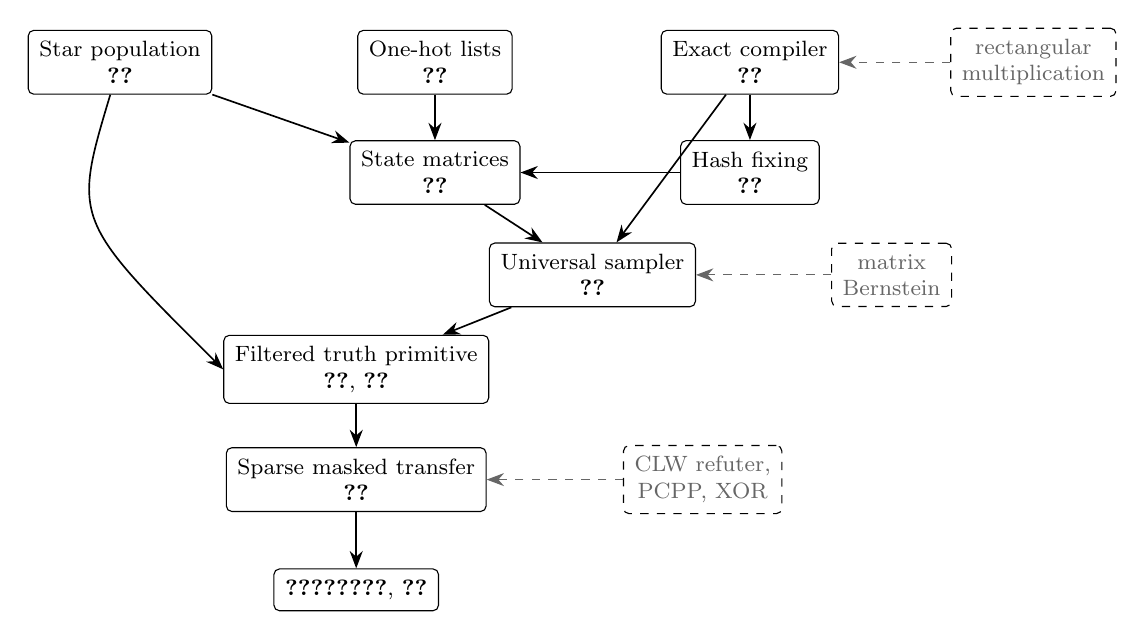
\begin{tikzpicture}[
  dep/.style={draw,rounded corners=2pt,align=center,inner sep=4pt,
    font=\footnotesize},
  imp/.style={draw,dashed,rounded corners=2pt,align=center,
    inner sep=4pt,font=\footnotesize,text=black!60},
  darr/.style={-{Stealth[length=2.2mm]},semithick},
  iarr/.style={-{Stealth[length=2.2mm]},dashed,black!60}]
\node[dep] (pop) at (0,4.6) {Star population\\ \cref{star:population}};
\node[dep] (list) at (4.0,4.6) {One-hot lists\\ \cref{list:repair}};
\node[dep] (comp) at (8.0,4.6) {Exact compiler\\ \cref{alg:section}};
\node[imp] (will) at (11.6,4.6) {rectangular\\ multiplication};
\node[dep] (hash) at (8.0,3.2) {Hash fixing\\ \cref{filt:soft}};
\node[dep] (mat) at (4.0,3.2) {State matrices\\ \cref{row:appendix}};
\node[dep] (samp) at (6.0,1.9) {Universal sampler\\ \cref{samp:printable}};
\node[imp] (tropp) at (9.8,1.9) {matrix\\ Bernstein};
\node[dep] (prim) at (3.0,0.7) {Filtered truth primitive\\ \cref{lem:primitive}, \cref{prim:ledger}};
\node[dep] (tr) at (3.0,-0.7) {Sparse masked transfer\\ \cref{tr:appendix}};
\node[imp] (clw) at (7.4,-0.7) {CLW refuter,\\ PCPP, XOR};
\node[dep] (thm) at (3.0,-2.1) {\cref{thm:tradeoff,thm:endpoint,thm:slow,thm:poly}, \cref{cor:gates}};
\draw[darr] (pop) -- (mat);
\draw[darr] (list) -- (mat);
\draw[darr] (comp) -- (hash);
\draw[darr] (hash) -- (mat);
\draw[darr] (mat) -- (samp);
\draw[darr] (comp) -- (samp);
\draw[darr] (samp) -- (prim);
\draw[darr] (pop) .. controls (-0.6,2.6) .. (prim.west);
\draw[darr] (prim) -- (tr);
\draw[darr] (tr) -- (thm);
\draw[iarr] (will) -- (comp);
\draw[iarr] (tropp) -- (samp);
\draw[iarr] (clw) -- (tr);
\end{tikzpicture}
\caption{\textbf{Dependency structure of the proof.} Solid boxes are
proved in this paper's appendices; dashed boxes are imported
interfaces, stated explicitly where they are used. The star
population bound enters twice: it shapes the state matrices and sets
the budget $B$ of the resource ledger.}
\label{fig:dag}
\end{figure}

\begin{table}[tp]
\centering
\small
\begin{tabular}{@{}lll@{}}
\toprule
Symbol & Meaning & Set in\\
\midrule
$n$ & final language length & \S\ref{sec:results}\\
$L,v$ & $\lceil\log_2(\cdot+2)\rceil$;\ $\max\{2,\log_2^*\cdot\}$, at the ambient length & \S\ref{sec:results}\\
$c$ & advantage exponent: forbidden agreement $1/2+L^{-c}$ & \S\ref{sec:results}\\
$K_{0,i},K_{i,\mathrm{alg}},K_i$ & native, algorithmic, and target denominator exponents & \S\ref{sec:results}, \S\ref{sec:transfer-overview}\\
$A_T,A_S$; $a_T,a_S$ & arbitrary fixed multipliers; endpoint coefficients & \S\ref{sec:results}\\
$W$; $G$ & physical wires (all occurrences); bottom-gate occurrences & \S\ref{sec:results}\\
$q$ & native input length of the counting algorithm & \S\ref{sec:stars-overview}\\
$r$; $b,s$ & number of Hamming blocks (even); block size $b=2^s{-}1$ & \S\ref{sec:stars-overview}\\
$k$; $N$ & live width $rs$; live points per side $N=2^{k/2}$ & \S\ref{sec:stars-overview}\\
$z,u,v$ & column (center) address; left and right star choices & \S\ref{sec:stars-overview}\\
$B$ & regular-filter threshold (with an enlarged count-list cap) & \S\ref{sec:count-overview}\\
$d_S,d_T$ & base Boolean degrees of the count lists & \S\ref{sec:count-overview}\\
$Q$; $h$; $\eta$ & sample count; trace-moment order ($h=4$); sampler accuracy & \S\ref{sec:count-overview}\\
$\overline\Lambda$; $\tau$ & reconstruction coefficient mass; its exponent $\overline\Lambda=O(L^\tau)$ & \S\ref{sec:transfer-overview}\\
$t$; $e_t$ & XOR power; reconstruction advantage threshold & \S\ref{sec:transfer-overview}\\
$\beta,\xi,\zeta,\delta$ & mask discard, filter error, XOR closeness, sparsification error & \S\ref{sec:transfer-overview}\\
\bottomrule
\multicolumn{3}{@{}p{0.94\textwidth}@{}}{\rule{0pt}{2.4ex}\footnotesize
Two letters are reused: $v$ is the slowly varying scale in the
theorems and the right star choice inside the algorithm; $s$ is the
block exponent in \S\ref{sec:stars-overview} and the sparse support
size in \S\ref{sec:transfer-overview}. The uses are local and never
meet in one formula.}\\
\end{tabular}
\caption{Recurring symbols, in order of appearance.}
\label{tab:notation}
\end{table}

\section{Relation to earlier work and attribution}
\label{sec:related}

Throughout this section and the appendices, four levels of ownership
are distinguished: \emph{classical tools} used as published,
\emph{inherited architecture} whose design is due to earlier authors,
\emph{adapted interfaces} restated here because their hypotheses
change, and \emph{new lemmas} proved in this paper. Each named
ingredient below is assigned to one of these levels.

The algorithm-to-lower-bound program converts nontrivial circuit
algorithms into circuit lower bounds; Williams's framework is a principal
source of this approach and of the rectangular multiplication tool used
here~\cite{WilliamsRect}. For depth-two threshold circuits, the
restriction and circuit-algorithm work of Kane--Williams and
Chen--Tal--Wang is fundamental~\cite{KaneWilliams,CTW}. The
almost-everywhere correlation transfer used here follows
Chen--Lyu--Williams~\cite{CLW}, including its reconstruction form of XOR
amplification, canonical recovery, and weak simulation/refutation
framework. We do not claim a new hardness amplification theorem, PCP of
proximity, or time hierarchy theorem.

\paragraph{Relation to the near-cubic wire manuscript.}
The companion manuscript~\cite{NagCubic} supplies deterministic
count-list constructions, the signed exact-equation printer, and a
componentwise implementation of the almost-everywhere transfer. It gives
near-cubic wire bounds with inverse-polynomial correlation. The present
paper changes the residual population and the way its observable is
contracted. It imports the exact equation decomposition and the
rectangular printing architecture; the star-cell mixed difference,
unconditional list repair, fixed-moment contraction, and sparse masked
transfer are proved here. We restate the parts of the old interfaces
whose hypotheses change, instead of assuming that their original
statements already cover nonlinear cells or malformed lists.

\paragraph{Relation to the gate preprint and the fan-in note.}
The gate preprint~\cite{NagGate} gives one language that is almost
everywhere hard for exact computation at positive-coefficient gate caps
$n^{5/2}/L^9$ for THR and $n^{5/2}/L^{9/2}$ for SYM. Row A improves
these denominators to $L^5$ and $L^4$ (\cref{cor:gates}) and
strengthens exact-computation
hardness to fixed-advantage correlation hardness. Its length guarantee
was already almost everywhere. The gate preprint is distinct from the
touching/fan-in working note~\cite{NagTouching}, which organizes
restriction bounds by the fan-ins and isolates the square-root survivor
cost. The new bound supersedes those quantitative gate
consequences, while continuing to use their circuit and printer
conventions. Neither work is required by any proof in this paper:
every imported interface has its primary statement in the near-cubic
companion manuscript~\cite{NagCubic}, and the one construction also
available in the gate preprint is cited only as a redundant second
source. The sole manuscript dependency of this paper is
\cite{NagCubic}.

\paragraph{Where the individual tools come from.}
The partition into radius-one stars is the classical perfect Hamming
code~\cite{Hamming}. The useful circuit estimate is the mixed-difference
bound across two groups of its blocks. Integer normalization of real
threshold functions is classical~\cite{MurogaTodaTakasu}.
That a threshold function decomposes into a disjoint union of exact
threshold functions goes back qualitatively to
Hansen--Podolskii~\cite{HansenPodolskii}; the particular
first-crossing construction used here is due to
Chen--Williams~\cite[Proposition 18(2), Appendix B]{ChenWilliams},
and its explicit form and signed printing implementation are imported
from \cite{NagCubic,NagGate}. Low-degree probabilistic counting is related
to the polynomial method of Alman--Williams~\cite{AlmanWilliams};
the nested-hash count-list interface used here is the one proved in
\cite{NagCubic}. Our matrix estimate is an application of Tropp's
rectangular matrix Bernstein inequality~\cite[Theorem 1.6]{Tropp},
not a new concentration inequality. The product-to-parity identity is
elementary Fourier expansion on the Boolean cube. Our use of it depends
on preserving the true range of a whole integer expression before
expansion. The novelty is in these compositions and their quantitative
and correlation-safe implementations.

\section{A partition that charges mixed dependence}
\label{sec:stars-overview}

Let the native input length be $q$. Partition most input coordinates
into an even number $r$ of blocks of size $b=2^s-1=\Theta(q/r)$.
A Hamming-code coset partitions each block into sets
$\{z,z+e_1,\ldots,z+e_b\}$. Products of these stars partition the
whole cube into $2^{q-k}$ equal cells of size $2^k$, where $k=rs$.
The unused input coordinates remain part of the cell address. Give half
the blocks to a live left variable $u$ and half to a live right variable
$v$; each has $N=2^{k/2}$ choices. Addition in input arguments is XOR.

For a bottom threshold $T_i$ define
\[
\Delta_i(z,u,v)=T_i(z+u+v)-T_i(z+u)-T_i(z+v)+T_i(z).
\]
The four underlying real scores form an additive rectangle.
Consequently $\Delta_i\in\{-1,0,1\}$. Writing its positive and
negative indicators as $Z_i^+,Z_i^-$ gives an exact identity for a
weighted top score:
\begin{equation}
\sum_i w_iT_i(z+u+v)
=A_z(u)+B_z(v)+\sum_i w_i(Z_i^+-Z_i^-).
\label{eq:mixed-score}
\end{equation}
The one-sided terms may be arbitrarily complicated functions of their
own live half and the column $z$. We never encode a dictionary of them.
\Cref{fig:stars} shows the geometry.

\begin{figure}[t]
\centering
\begin{minipage}[b]{0.64\textwidth}
\centering
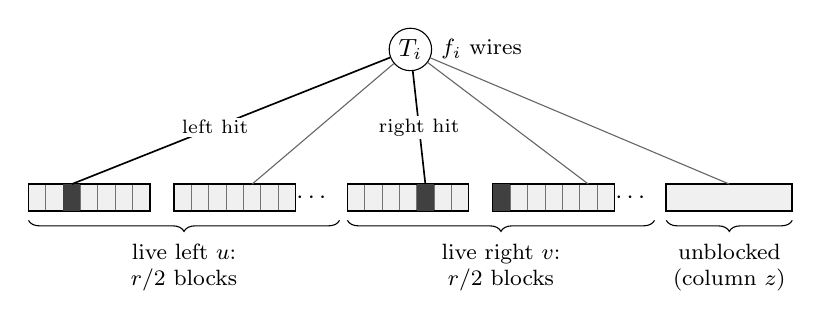
\begin{tikzpicture}[font=\small]
% four visible blocks of b=7 cells; light cells are code-center bits
\foreach \bx in {0,1.85,4.05,5.9} {
  \foreach \i in {0,...,6}
    \draw[black!55,fill=black!6,line width=0.3pt]
      ({\bx+\i*0.22},0) rectangle ({\bx+\i*0.22+0.22},0.34);
  \draw[black,line width=0.6pt] (\bx,0) rectangle ({\bx+1.54},0.34);
}
% the live star choice: at most one flipped coordinate per block
\fill[black!75] (0.44,0) rectangle (0.66,0.34);   % left block 1: flip
\fill[black!75] (4.93,0) rectangle (5.15,0.34);   % right block 1: flip
\fill[black!75] (5.90,0) rectangle (6.12,0.34);   % right block 2: flip
\node at (3.62,0.17) {$\cdots$};
\node at (7.67,0.17) {$\cdots$};
% unblocked coordinates
\draw[black,fill=black!6,line width=0.6pt] (8.1,0) rectangle (9.7,0.34);
% one bottom threshold and its wires
\node[draw,circle,inner sep=1.5pt] (gate) at (4.85,2.05) {$T_i$};
\node[right=2pt,font=\footnotesize] at (5.05,2.05) {$f_i$ wires};
\draw[semithick] (gate) -- (0.55,0.34)
  node[pos=0.55,fill=white,inner sep=1pt,font=\scriptsize]{left hit};
\draw[black!60,thin] (gate) -- (2.84,0.34);
\draw[semithick] (gate) -- (5.04,0.34)
  node[pos=0.5,fill=white,inner sep=1pt,font=\scriptsize]{right hit};
\draw[black!60,thin] (gate) -- (7.11,0.34);
\draw[black!60,thin] (gate) -- (8.9,0.34);
% braces
\draw[decorate,decoration={brace,mirror,amplitude=4pt}] (0,-0.12) -- (3.95,-0.12)
  node[midway,below=5pt,align=center,font=\footnotesize]
  {live left $u$:\\ $r/2$ blocks};
\draw[decorate,decoration={brace,mirror,amplitude=4pt}] (4.05,-0.12) -- (7.95,-0.12)
  node[midway,below=5pt,align=center,font=\footnotesize]
  {live right $v$:\\ $r/2$ blocks};
\draw[decorate,decoration={brace,mirror,amplitude=4pt}] (8.1,-0.12) -- (9.7,-0.12)
  node[midway,below=5pt,align=center,font=\footnotesize]
  {unblocked\\ (column $z$)};
\end{tikzpicture}\\[2pt]
{\footnotesize (a)}
\end{minipage}\hfill
\begin{minipage}[b]{0.335\textwidth}
\centering
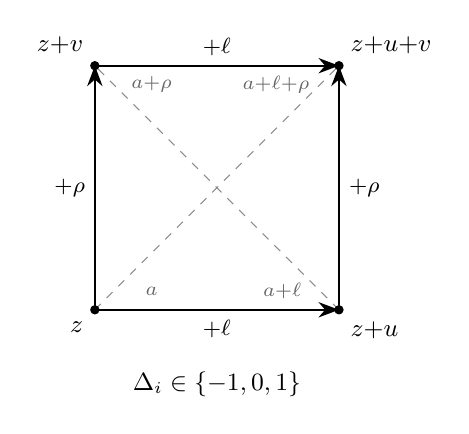
\begin{tikzpicture}[font=\small]
\coordinate (z) at (0,0);
\coordinate (zu) at (3.1,0);
\coordinate (zv) at (0,3.1);
\coordinate (zuv) at (3.1,3.1);
\draw[dashed,black!45] (z) -- (zuv);
\draw[dashed,black!45] (zu) -- (zv);
\draw[flow] (z) -- (zu) node[midway,below,font=\footnotesize]{$+\ell$};
\draw[flow] (zv) -- (zuv) node[midway,above,font=\footnotesize]{$+\ell$};
\draw[flow] (z) -- (zv) node[midway,left,font=\footnotesize]{$+\rho$};
\draw[flow] (zu) -- (zuv) node[midway,right,font=\footnotesize]{$+\rho$};
\foreach \p in {z,zu,zv,zuv} \fill (\p) circle (1.7pt);
\node[below left=1pt] at (z) {$z$};
\node[below right=1pt] at (zu) {$z{+}u$};
\node[above left=1pt] at (zv) {$z{+}v$};
\node[above right=1pt] at (zuv) {$z{+}u{+}v$};
\node[font=\scriptsize,text=black!60] at (0.72,0.24) {$a$};
\node[font=\scriptsize,text=black!60] at (2.38,0.24) {$a{+}\ell$};
\node[font=\scriptsize,text=black!60] at (0.72,2.86) {$a{+}\rho$};
\node[font=\scriptsize,text=black!60] at (2.30,2.86) {$a{+}\ell{+}\rho$};
\node[align=center] at (1.55,-0.95) {$\Delta_i\in\{-1,0,1\}$};
\end{tikzpicture}\\[2pt]
{\footnotesize (b)}
\end{minipage}
\caption{\textbf{Star cells and the mixed residual.}
(a) Most of the $q$ input coordinates are grouped into $r$ Hamming
blocks of $b=2^s{-}1$ coordinates. The column address selects a code
center: every light cell is a center bit determined by $z$, as are the
unblocked coordinates. A live point flips at most one coordinate per
block (dark cells); the $r/2$ left choices form $u$ and the $r/2$
right choices form $v$, giving $2^{k/2}$ points per side with $k=rs$.
For a bottom threshold reading $f_i$ wires, the mixed difference
$\Delta_i$ is nonzero only when the flipped coordinate on \emph{each}
side is a relevant hit; averaged over the coset and the cell this has
probability $O(r^{3/2}f_i/q^{3/2})$ (\cref{star:population}).
(b) For fixed $(z,u,v)$, the four corner scores of one threshold form
an additive rectangle: adding $u$ contributes $\ell$ on both horizontal
sides and adding $v$ contributes $\rho$ on both vertical sides. Equal
diagonal score sums forbid the alternating sign patterns, so
$\Delta_i=T_i(z{+}u{+}v)-T_i(z{+}u)-T_i(z{+}v)+T_i(z)\in\{-1,0,1\}$
(\cref{star:range}).}
\label{fig:stars}
\end{figure}

\paragraph{A two-block example.}
Take $r=2$: one left block and one right block, center $z$, left flip
$u$ at coordinate $i$, right flip $v$ at coordinate $j$. Consider
first a threshold that reads only left coordinates. Its value may
change arbitrarily with $u$---the gate varies across the cell---but
$T(z{+}u{+}v)=T(z{+}u)$ and $T(z{+}v)=T(z)$, so $\Delta_T=0$: all of
that variation is absorbed into the one-sided term $A_z(u)$ at no
cost. Now take $T=\ind[x_i+x_j\ge2]$ with both flips raising their
coordinate from $0$ to $1$. The corner scores are $0,1,1,2$, the
outputs are $0,0,0,1$, and $\Delta_T=+1$. In contrast, for
$T=\ind[x_i+x_j\ge1]$, the same corners have outputs $0,1,1,1$
and $\Delta_T=-1$: either flip alone already crosses the threshold.
In both cases, the effect of one side changes with the setting of the
other. Charging circuits only for this mixed dependence, rather than
for every gate that varies on a cell, is the source of the $3/2$ power in
\cref{eq:star-population-main}. This is the partition's instance of
the absorption principle of \cref{sec:results}: one-sided complexity
costs nothing; only coincidences enter the budget.

The total influence of a threshold on $f$ variables is at most $\sqrt f$.
A mixed difference additionally requires the other half to hit its
support. Averaging the code coset and the input gives
\begin{equation}
\Pr[\Delta_i\ne0]\le
\frac{2\sqrt{f_i}}{b+1}\min\{1,f_i/(b+1)\}
\le O\!\left(\frac{r^{3/2}f_i}{q^{3/2}}\right).
\label{eq:star-population-main}
\end{equation}
Thus the mean number of nonzero signed residual coordinates is
$O(r^{3/2}W/q^{3/2})$. This bounds the mean of the pointwise residual
population, not the number of gates that vary somewhere on a cell.
Different rows can activate completely different gates. A deterministic
meet-in-the-middle computation finds a coset meeting the weighted mean
bound, even when many verifier coordinates have to share it.

For fixed $u,v$, the original input is an affine map over $\F_2$ of the
code-center bits. An original real threshold need not remain a real
threshold in those bits. This matters. We first decompose the original
threshold into disjoint exact equations, then pull back those equations.
Each pulled-back equation has an additive left and right score. The
printer uses sorted half-score lists, so this additive form suffices;
it does not require that the scores be linear in the new coordinates.

\section{Counting the joint observable}
\label{sec:count-overview}

The task of this section, stated before its machinery: given a tuple
of at most four circuits from the restricted class and the shared
masks constructed below, deterministically estimate the unnormalized
masked joint acceptance
\[
\E_{e,x}\Big[M(e,x)\prod_{i=1}^{a}C_i(x)\Big],\qquad a\le4,
\]
to inverse-polynomial accuracy, in time $2^{q-k/4}q^{O(1)}$---the
running-time saving the lower-bound transfer requires. Three glosses.
The masks $M$ are the paper's constructed filters, carrying their own
seeds $e$; they are not arbitrary. \emph{Unnormalized} means a
discarded input contributes zero: nothing is renormalized over the
retained inputs. And the tuple size four is exactly what the
componentwise transfer consumes, no more. Every construction in this
section exists to compute this one quantity within the stated load.

The pipeline follows one arc: separate one-sided behavior exactly,
control the interactions that remain, count them inside a fixed
budget, and hand the count to the hardness transfer.
\Cref{fig:pipeline} summarizes the six stages and the guarantee each
one hands to the next. The subsections below explain the three
nonstandard stages.

The following recurring terms have fixed meanings. A \emph{column} is one
cell's address $z$; its live choices $(u,v)$ index the points inside
that cell. The \emph{printer} is the exact batched evaluation
algorithm of \cref{alg:section}: it recovers an integer conditional
potential at every column through sorted half-score lists and
rectangular multiplication. The \emph{load} is the logarithm of the
expanded occurrence count of the expression handed to the printer;
the printer applies while the load stays inside a fixed small linear
allowance in $q$. A \emph{count list} is a vector of Boolean
indicators reporting one candidate residual count, and its
\emph{reported state} is the coordinate the list singles
out---after the repair below, exactly one on every input and every
seed. A \emph{selector} is a bounded one-sided coefficient vector
multiplying a state matrix; the sampler is accurate for all of them
at once. \emph{Carrier} circuits, which appear only in the transfer,
are the restricted or complemented atoms that a reconstruction
assigns to one named proof coordinate.

\begin{figure}[tp]
\centering
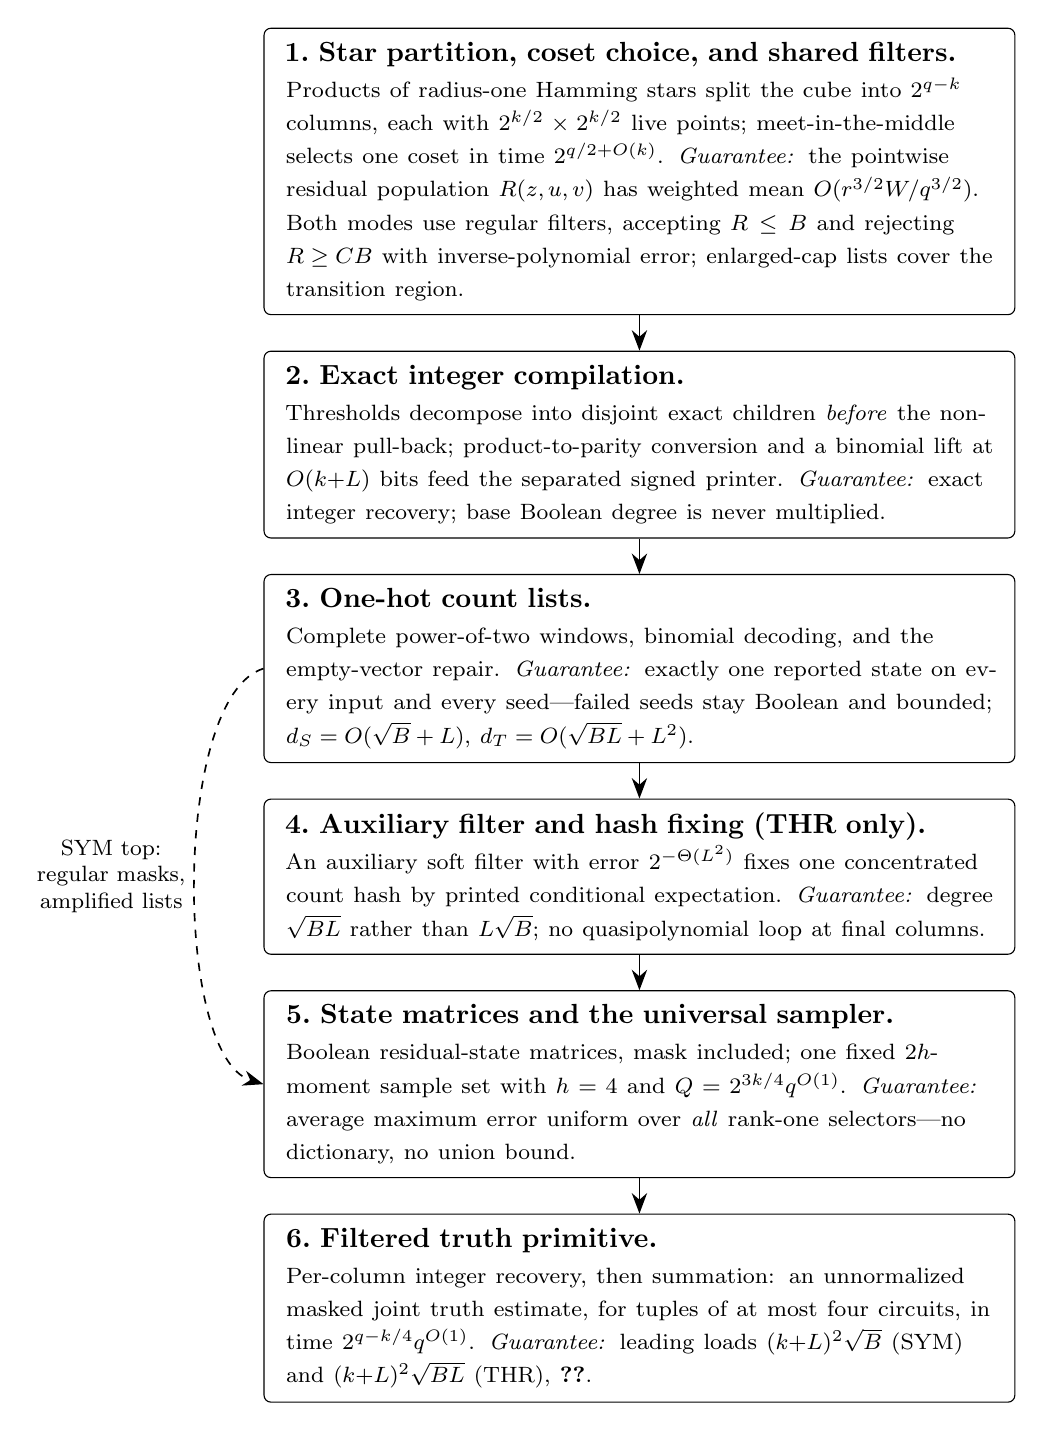
\begin{tikzpicture}[node distance=4.5mm]
\node[stage] (s1) {\textbf{1.\ Star partition, coset choice, and shared filters.}\\[1pt]
\footnotesize Products of radius-one Hamming stars split the cube into
$2^{q-k}$ columns, each with $2^{k/2}\times2^{k/2}$ live points;
meet-in-the-middle selects one coset in time $2^{q/2+O(k)}$.
\emph{Guarantee:} the pointwise residual population $R(z,u,v)$ has
weighted mean $O(r^{3/2}W/q^{3/2})$. Both modes use regular filters,
accepting $R\le B$ and rejecting $R\ge CB$ with inverse-polynomial
error; enlarged-cap lists cover the transition region.};
\node[stage,below=of s1] (s2) {\textbf{2.\ Exact integer compilation.}\\[1pt]
\footnotesize Thresholds decompose into disjoint exact children
\emph{before} the nonlinear pull-back; product-to-parity conversion and
a binomial lift at $O(k{+}L)$ bits feed the separated signed printer.
\emph{Guarantee:} exact integer recovery; base Boolean degree is never
multiplied.};
\node[stage,below=of s2] (s3) {\textbf{3.\ One-hot count lists.}\\[1pt]
\footnotesize Complete power-of-two windows, binomial decoding, and the
empty-vector repair. \emph{Guarantee:} exactly one reported state on
every input and every seed---failed seeds stay Boolean and bounded;
$d_S=O(\sqrt B+L)$, $d_T=O(\sqrt{BL}+L^2)$.};
\node[stage,below=of s3] (s4) {\textbf{4.\ Auxiliary filter and hash fixing (THR only).}\\[1pt]
\footnotesize An auxiliary soft filter with error $2^{-\Theta(L^2)}$ fixes one
concentrated count hash by printed conditional expectation.
\emph{Guarantee:} degree $\sqrt{BL}$ rather than $L\sqrt B$; no
quasipolynomial loop at final columns.};
\node[stage,below=of s4] (s5) {\textbf{5.\ State matrices and the universal sampler.}\\[1pt]
\footnotesize Boolean residual-state matrices, mask included; one fixed
$2h$-moment sample set with $h=4$ and $Q=2^{3k/4}q^{O(1)}$.
\emph{Guarantee:} average maximum error uniform over \emph{all} rank-one
selectors---no dictionary, no union bound.};
\node[stage,below=of s5] (s6) {\textbf{6.\ Filtered truth primitive.}\\[1pt]
\footnotesize Per-column integer recovery, then summation: an
unnormalized masked joint truth estimate, for tuples of at most four
circuits, in time $2^{q-k/4}q^{O(1)}$.
\emph{Guarantee:} leading loads $(k{+}L)^2\sqrt B$ (SYM) and
$(k{+}L)^2\sqrt{BL}$ (THR), \cref{eq:loads-main}.};
\draw[flow] (s1) -- (s2);
\draw[flow] (s2) -- (s3);
\draw[flow] (s3) -- (s4);
\draw[flow] (s4) -- (s5);
\draw[flow] (s5) -- (s6);
\draw[flow,dashed] (s3.west) .. controls +(-1.15,-0.35) and +(-1.15,0.35) .. (s5.west)
  node[pos=0.5,left,align=center,font=\footnotesize]{SYM top:\\regular masks,\\amplified lists};
\end{tikzpicture}
\caption{\textbf{The counting pipeline.} Each stage's guarantee is what
the next stage consumes; the SYM mode retains the shared regular filters
and skips only the auxiliary hash-fixing stage. The
italicized guarantees are the three compiler invariants proved in
\cref{list:repair}, \cref{filt:soft}, and \cref{samp:printable},
combined in the resource ledger of \cref{prim:ledger}.}
\label{fig:pipeline}
\end{figure}

\subsection{Lists whose failed outputs are still bounded}
For residual weight at most $B$, a nested hash encodes the count with
Boolean polynomials of degree $O(\sqrt B+L)$ at fixed failure
probability; this count-list mechanism descends from the
probabilistic-polynomial line of Alman--Williams and
Chen--Tal--Wang~\cite{AlmanWilliams,CTW}, in the deterministic
implementation of~\cite{NagCubic}.
The source proof only uses the actual set of input ones, so it applies
to the pointwise population in \cref{eq:star-population-main}.
Its interpolation outside a certified discrepancy interval, however,
need not give a one-hot vector. We replace every interval by a complete
power-of-two window, decode its binary residue with binomial
polynomials, and assign an empty reconstructed vector to the zero-count
state. This costs only a constant factor in degree and makes the list
exactly one-hot on every input and every seed.

This repair justifies equalities over the integers, not only over
$\F_2$. A symmetric lookup and a tuple of radix counts now remain
Boolean even when their value is incorrect. To amplify a SYM list, we
expand coordinatewise majority over the integers before converting
products to parities. The base Boolean degree stays
$d_S=O(\sqrt B+L)$; the number of factors adds precision bits instead.
For THR, a deterministic higher-moment hash construction gives
$d_T=O(\sqrt{BL}+L^2)$ with inverse-polynomial average error. Its radix
tuple products are likewise flattened before parity conversion.

\subsection{Why there are two filters}
A THR top is evaluated through polynomially many exact-equation and
modular rows. Bounded individual states do not make the sum of failed
rows bounded by one. We therefore estimate the \emph{filtered truth
observable}, not an unfiltered sum with a population-exception error.
A regular Boolean sparsity filter accepts populations at most $B$ and
rejects populations above a fixed multiple $CB$, with inverse-polynomial
error. The count lists have the enlarged cap, covering the entire
transition interval. All rows and all monomials for one named verifier
coordinate use the same filter.

To choose a single high-confidence THR hash, a second, softer filter
accepts weight at most $CB$ and rejects weight above $C^2B$. Its error
is $2^{-\Theta(L^2)}$, small enough to dominate the unconditional range
of the discrepancy moment potential. This auxiliary filter is expanded
inside a printed conditional expectation. Its quasipolynomial seed
space is never enumerated at each column in the final counting pass.
This separation is what permits $\sqrt{BL}$, rather than an amplified
$L\sqrt B$, in the THR degree.

\subsection{A universal sampler instead of a selector dictionary}
For a fixed column and state, let $D$ be the $N\times N$ Boolean matrix
of residual-state indicators, including the regular mask. After Fourier
expansion of a SYM lookup, or of a THR modular equality, the remaining
one-sided dependence has the form $a_u b_v$ with $|a_u|,|b_v|\le1$.
For sampled entries $(U_j,V_j)$ put
\[
E_D=QD-N^2\sum_{j=1}^Q D(U_j,V_j)e_{U_j}e_{V_j}^{\mathsf T}.
\]
The error in the normalized bilinear observable is then, exactly,
\[
\left|\frac{a^{\mathsf T}Db}{N^2}
-\frac1Q\sum_{j=1}^Q a_{U_j}b_{V_j}D(U_j,V_j)\right|
=\frac{|a^{\mathsf T}E_Db|}{QN^2}
\le\frac{\|E_D\|}{QN},
\]
simultaneously for \emph{all} such $a,b$: entries of modulus at most
one give $\|a\|_2,\|b\|_2\le\sqrt N$, so the operator norm alone
controls every bilinear test at once, including selectors chosen
after the sample list is fixed. In
particular, a selector may depend on the column, on the chosen
sampler, and on all one-sided gate values. There is no independence
assumption and no union bound over a dictionary of selectors. This is
the sampler's instance of the absorption principle: the arbitrary
one-sided behavior absorbed in \cref{sec:stars-overview} reappears
here inside the selectors, and one fixed sample list handles all of
it---accuracy is bought once, with samples, not per selector with
error.

For $I=q^{O(1)}$ state matrices, Tropp's inequality and a $2h$-th
trace moment give an average maximum operator error at most $\eta$ with
\begin{equation}
Q=O\!\left(Nh\eta^{-2}(4N^2I)^{1/h}\right).
\label{eq:sample-main}
\end{equation}
We take $h=4$, a fixed constant, and pay the dimension factor through
$Q=2^{3k/4}q^{O(1)}$. The resulting counting pass costs
$2^{q-k/4}q^{O(1)}$. Taking $h$ logarithmic in the dimension would
unnecessarily spend a logarithm in the printer's precision.

The trace potential is a polynomial in at most $2h$ sample-position
indicators per term. A $2h$-wise independent finite-field generator
therefore preserves its expectation. Conditional probabilities after
fixing seed bits are computed by binary Gaussian elimination. Greedy
conditional expectation fixes one sampler for every column. After a
common integer scaling, the potential is nonnegative and has bit length
$O(k+L)$ \emph{per column}. The printer recovers this integer at each
column before summing the columns. It never tries to recover the global
sum using the same modulus.

\subsection{The numerical law}
Product-to-parity conversion preserves the base Boolean degree, and
binomial lifting at $O(k+L)$ bits of precision produces the leading
printer costs
\begin{equation}
(k+L)^2\sqrt B\quad\text{for SYM},\qquad
(k+L)^2\sqrt{BL}\quad\text{for THR}.
\label{eq:loads-main}
\end{equation}
All additive polylogarithmic terms, signed coefficient lengths, and
expanded occurrence counts are retained in the appendices. In
particular, the number of expanded terms is not substituted for the
range of the unexpanded potential. Product-to-parity conversion is the
compiler's instance of the absorption principle: precision and term
count are paid; Boolean degree is not.

\section{From a counting algorithm to correlation hardness}
\label{sec:transfer-overview}

The conversion to hardness has a fixed shape. Fix any sufficiently
large length and suppose, for contradiction, that some circuit from a
target class within the wire cap agrees with the intended hard
function noticeably more often than chance at that length. A
reconstruction lemma converts that circuit into bounded approximations
of the coordinates of a PCP-style proof that a nondeterministic
computation accepts. The counting machinery of the previous sections
then lets one fixed weak machine \emph{verify} such a candidate proof
unusually fast---but the imported refuter framework of
Chen--Lyu--Williams~\cite{CLW} guarantees, at the corresponding source
length, an input on which fast weak verification must fail. The
contradiction rules out the violating circuit at the chosen length,
and running the same argument at every sufficiently large length gives
the almost-everywhere conclusion. The one nonstandard step is the
middle one: our counting primitive evaluates \emph{masked}
observables, which discard part of the input space, so a standard
counting-to-hardness theorem cannot be invoked as a black box.
Verification must remain sound when a dishonest witness influences
the masks, and complete when honest clause values lose masked mass;
both are proved for unnormalized masked scores in \cref{tr:appendix}.

The reconstruction lemma used in the almost-everywhere framework
produces bounded approximators of named proof coordinates as real
linear combinations of restricted or complemented circuit atoms.
Let $\overline\Lambda$ bound the coefficient mass. A fourth-moment
sparsification uses $s=O(\overline\Lambda^2)$ atoms per coordinate at a
fixed small $L^4$ error. This is an existential guessed witness; it does
not alter the hypothetical Boolean correlator. The same named
coordinate is used consistently at all of its occurrences.

The carrier for a coordinate has at most $s w+O(q^2)$ wires, where
$w$ is the cap for an individual atom. A weighted common-coset choice
gives a mean residual population at most
$O(r^{3/2}(s w+q^2)/q^{3/2})$. For a fixed small $\beta>0$ put
\begin{equation}
B=O\!\left(1+\frac{r^{3/2}(s w+q^2)}{\beta q^{3/2}}\right).
\label{eq:carrier-main}
\end{equation}
The regular mask for a coordinate discards incidence mass at most
$\beta+o(1)$. A clause uses the product of its two coordinate masks,
without renormalizing their accepted mass.

Two facts make this safe for unbounded real sparse witnesses. First,
the verifier checks masked second moments and a nonnegative polynomial
penalty for distance from a Boolean value. Cauchy--Schwarz then compares
every passing witness to one globally consistent Boolean proof.
Second, a Boolean clause value is nonnegative. Deleting it by a Boolean
mask cannot increase the soundness bound, even if the mask was chosen
from a dishonest witness. In completeness the discarded mass is charged
once against a bounded honest clause value. It is never multiplied by
$\overline\Lambda^4$, the mass of a polynomial expansion. That mass
affects only the requested inverse-polynomial numerical accuracy.
This is the transfer's instance of the absorption principle, and the
reason the structural gain of the partition survives amplification.

Substitute $w=q^{7/2}/H(q)$ and $k=\Theta(rL)$ in
\cref{eq:loads-main,eq:carrier-main}. With $K_{0,T}=5$ and $K_{0,S}=4$, the
leading load is
\begin{equation}
O\!\left(q\,r^{11/4}L^{K_{0,i}/2}
                 \frac{\overline\Lambda}{\sqrt{H(q)}}\right),
\qquad i\in\{T,S\}.
\label{eq:master-main}
\end{equation}
The exponent $11/4$ consists of $2$ from $k^2$ and $3/4$ from the
square root of the mixed-residual population. The threshold case pays
one further square root of $L$. The printer accepts a sufficiently
small fixed linear load; the main counting time is
$2^{q-k/4}q^{A}$ for a frozen constant $A$.

For the headline theorem choose a reconstruction mass
$\overline\Lambda=O(L^\tau)$ with
$c<\tau<\min\{(K_T-5)/2,(K_S-4)/2\}$ and intermediate cap exponents
$K_{0,i}+2\tau<K_{i,\mathrm{alg}}<K_i$. Take
$r=\Theta(\log L)$. The load is $o(q)$, the saving is
superpolynomial, and the strict exponent gaps absorb the logarithmic
arity dilation and every fixed multiplier. Row B is obtained with
$\tau=3/16$, $K_{T,\mathrm{alg}}=87/16$,
$K_{S,\mathrm{alg}}=71/16$; the remaining power of $L$ in the load
is $-1/32$. \Cref{fig:slack} displays this budget.

\begin{figure}[tp]
\centering
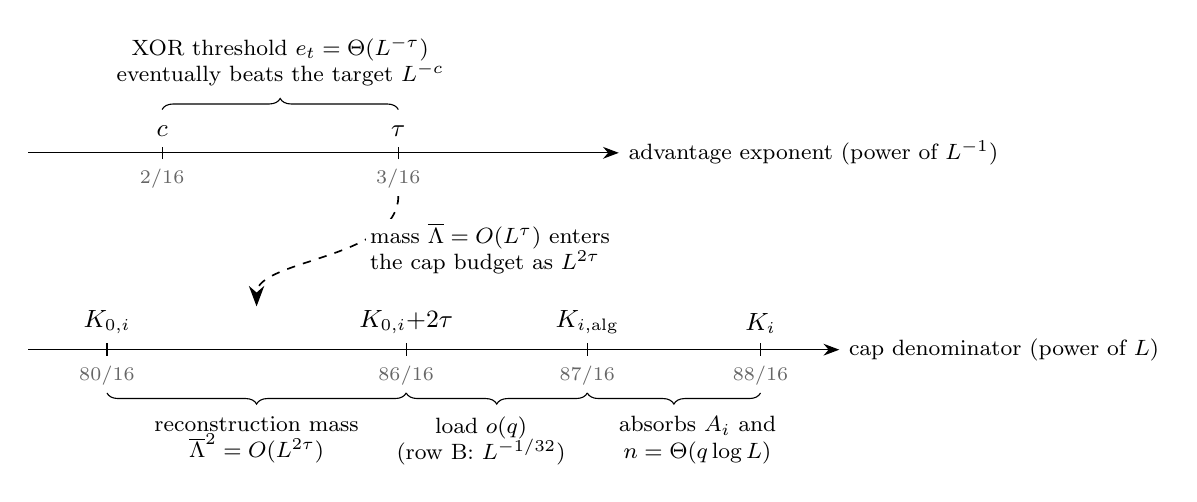
\begin{tikzpicture}[font=\small]
% top axis: advantage exponents
\draw[-{Stealth[length=2mm]}] (0.4,3.5) -- (7.9,3.5);
\node[right,font=\footnotesize] at (7.9,3.5) {advantage exponent (power of $L^{-1}$)};
\draw (2.1,3.42) -- (2.1,3.58) node[above] {$c$};
\draw (5.1,3.42) -- (5.1,3.58) node[above] {$\tau$};
\node[below,font=\scriptsize,text=black!60] at (2.1,3.42) {$2/16$};
\node[below,font=\scriptsize,text=black!60] at (5.1,3.42) {$3/16$};
\draw[decorate,decoration={brace,amplitude=4pt}] (2.1,4.05) -- (5.1,4.05)
  node[midway,above=5pt,font=\footnotesize,align=center]
  {XOR threshold $e_t=\Theta(L^{-\tau})$\\ eventually beats the target $L^{-c}$};
% connector
\draw[flow,dashed] (5.1,2.95) .. controls (5.1,2.15) and (3.3,2.15) .. (3.3,1.55)
  node[pos=0.4,right=6pt,font=\footnotesize,align=left,
       fill=white,inner sep=1.5pt]
  {mass $\overline\Lambda=O(L^{\tau})$ enters\\ the cap budget as $L^{2\tau}$};
% bottom axis: cap denominator exponents
\draw[-{Stealth[length=2mm]}] (0.4,1.0) -- (10.7,1.0);
\node[right,font=\footnotesize] at (10.7,1.0) {cap denominator (power of $L$)};
\draw (1.4,0.92) -- (1.4,1.08) node[above] {$K_{0,i}$};
\draw (5.2,0.92) -- (5.2,1.08) node[above] {$K_{0,i}{+}2\tau$};
\draw (7.5,0.92) -- (7.5,1.08) node[above] {$K_{i,\mathrm{alg}}$};
\draw (9.7,0.92) -- (9.7,1.08) node[above] {$K_i$};
\node[below,font=\scriptsize,text=black!60] at (1.4,0.92) {$80/16$};
\node[below,font=\scriptsize,text=black!60] at (5.2,0.92) {$86/16$};
\node[below,font=\scriptsize,text=black!60] at (7.5,0.92) {$87/16$};
\node[below,font=\scriptsize,text=black!60] at (9.7,0.92) {$88/16$};
% braces below
\draw[decorate,decoration={brace,mirror,amplitude=4pt}] (1.4,0.45) -- (5.2,0.45)
  node[midway,below=5pt,font=\footnotesize,align=center]
  {reconstruction mass\\ $\overline\Lambda^2=O(L^{2\tau})$};
\draw[decorate,decoration={brace,mirror,amplitude=4pt}] (5.2,0.45) -- (7.5,0.45)
  node[midway,below=5pt,xshift=-2mm,font=\footnotesize,align=center]
  {load $o(q)$\\ (row B: $L^{-1/32}$)};
\draw[decorate,decoration={brace,mirror,amplitude=4pt}] (7.5,0.45) -- (9.7,0.45)
  node[midway,below=5pt,xshift=3mm,font=\footnotesize,align=center]
  {absorbs $A_i$ and\\ $n=\Theta(q\log L)$};
\end{tikzpicture}
\caption{\textbf{Where the strict inequalities of \cref{thm:tradeoff}
are spent} (spacing not to scale). The gap $c<\tau$ on the advantage
axis lets the reconstructed XOR threshold eventually beat the forbidden
advantage. The mass $\overline\Lambda=O(L^\tau)$ then enters the
denominator budget squared, moving the usable exponent from $K_{0,i}$
to $K_{0,i}+2\tau$; the gap to $K_{i,\mathrm{alg}}$ makes the master
load \cref{eq:master-main} vanish relative to $q$; and the final gap to
$K_i$ absorbs every fixed multiplier together with the arity dilation.
Small numbers show row~B for $\THR\circ\THR$ ($c=1/8$, $\tau=3/16$, in
sixteenths); the SYM values are $64/16$, $70/16$, $71/16$, $72/16$.}
\label{fig:slack}
\end{figure}

At the constant-advantage endpoint, fix the required saving first,
choose a sufficiently large \emph{constant} $r$, then choose the cap
coefficients small enough for \cref{eq:master-main}. The coefficients
are not uniform over all savings. In row C choose
$r=\Theta(v^{1/16})$, mass $O(v^{1/8})$, and an intermediate
denominator $L^{K_{0,i}}v^{3/4}$; the load has a factor $v^{-5/64}$.
For the native range $0<\varepsilon\le1/2$ of row D, take
$c<\tau<e/2<\varepsilon/2$, mass $O(q^\tau)$,
intermediate cap $q^{7/2-e}$, and $r=\Theta(L)$; the remaining
polynomial load exponent is $1-e/2+\tau<1$.
The extension to $\varepsilon>1/2$ is \cref{cor:poly-prior}.

For each regime we freeze one weak machine with both circuit-class
modes. The canonical source object is selected before its class mode,
so the resulting language is common to both classes. The external
almost-everywhere refuter, systematic encoding, XOR reconstruction, and
canonical recovery are exactly the roles imported from
\cite{CLW,NagCubic,NagGate}. The appendix states the semantic interface,
proves the new masked verification step, and records the parameter and
length changes separately.

\section{Limitations and verification scope}
\label{sec:limitations-main}

The following obstructions are included with proofs, and with their
scope deliberately limited. They do not prove an optimal lower-bound
frontier for these circuit classes.

\begin{itemize}
\item At the log-free $a n^{7/2}$ wire scale, a Slepian comparison
supplies polynomial-bit threshold representations for which every
positive-dimensional affine restriction has a large population of
nonconstant original bottom gates. Affine restrictions cannot make a
square-root charge in this population sublinear in $n$; other residual
representations or charges remain open. The represented Boolean bottom
functions can be chosen distinct even up to complementation; the claim
concerns this bottom layer, not the complexity of its top observable.
\item The $O(\overline\Lambda^2)$ sparse support above is sharp for
constant-error approximation in the general bounded-dictionary model:
a finite Boolean slice forces $\Omega(\overline\Lambda^2)$ support.
This is not a uniform-cube circuit lower bound.
\item For random homogeneous thresholds and an equal-weight
symmetric top, an exact Krawtchouk expansion describes the aggregate
counting law. The coefficients are layer coefficients, with no extra
binomial multiplicity. Adaptive THR top weights defeat an inference
from that equal-weight law: they can select a dictator-like component.
The calculation is a random-instance statement, not a worst-case
algorithm for unrestricted weighted tops.
\end{itemize}

These facts explain why a stronger gate exponent or a log-free
$n^{7/2}$ wire coefficient does not follow merely by changing a
retention parameter, applying an aggregate Gaussian heuristic, or
sparsifying the reconstruction more aggressively. The present method
still pays a square-root cost for its genuinely mixed residuals.

\paragraph{Verification and artifacts.}
The manuscript is a conventional mathematical proof. It separates
three kinds of claim: identities proved here in full, quantitative
compiler contracts whose resource accounting is displayed, and
imported lower-bound interfaces stated explicitly where they are
used. Finite exact-arithmetic checks of
decoder one-hotness, residual signs, and conditional potentials are
useful implementation checks; they are not substitutes for the proofs.
No statement in this manuscript is asserted to be Lean- or otherwise
kernel-checked. The earlier gate preprint's mechanization discussion
does not establish a formalization of this paper. A natural single
future formalization target is row B with the explicit intermediate
parameters above; such a future artifact would need to state precisely
which imported interfaces remain axioms.

\paragraph{Use of generative AI.}
This work was carried out with substantial assistance from
large-language-model systems from OpenAI and Anthropic, used for
mathematical exploration, drafting and revision of the manuscript,
implementation of the finite exact-arithmetic checks, and iterated
adversarial review of the arguments, under the author's direction.
Machine-generated text, proofs, and review reports were treated as
untrusted input: every mathematical claim in this manuscript is
presented with an explicit proof or an explicitly labeled imported
interface, and the author takes full responsibility for all content.
No generated output is offered as a proof certificate.

\section{Open targets}
\label{sec:open}

Each target below names the specific quantitative barrier inside the
present proof, so that progress on it is checkable against the stated
equations.

\begin{enumerate}
\item \textbf{The log-free wire endpoint.} Remove the denominators in
row A entirely: a fixed-coefficient $n^{7/2}$ wire cap at constant
advantage. In \cref{eq:master-main} the factor $r^{11/4}$ collects two
powers of $r$ from the printer precision $k^2$ with $k=\Theta(rL)$,
and three quarters of a power from the square root of the
mixed-residual population; the native powers $K_{0,T}=5$ and
$K_{0,S}=4$ are what absorb these costs. A printer recovering
conditional potentials at amortized precision $o(k+L)$, or a
contraction of genuinely mixed residuals cheaper than the square
root, would each remove part of the denominator. \Cref{lim:appendix}
closes one further route: in the general bounded-dictionary model the
sparse-witness support cannot be reduced below
$\Omega(\overline\Lambda^{2})$.

\item \textbf{Every multiplier at the endpoint powers.} Close the gap
between rows A and B. At the exact powers $5$ and $4$ the load in
\cref{eq:master-main} is linear in $q$ with a fixed constant
multiplier, and the printer tolerates only a sufficiently small fixed
linear load; this is exactly what forces the coefficients of
\cref{thm:endpoint} to be chosen after the required saving. The target
is a uniform, printer-compatible construction at these exact powers
that supports every fixed native coefficient, retains the polynomial
saving required by the fixed transfer, and absorbs final arity dilation.
It must yield one hard language independent of the coefficients:
$\exists F\,\forall A_T,A_S>0\,\exists n_0\,\forall n\ge n_0$,
not a separate language for each pair of coefficients.

\item \textbf{A gate exponent above $5/2$.} The wire theorems reach
gates only through $W\le(n+1)G$ (\cref{cor:gates}), which is lossy
precisely when the average fan-in is sublinear.
\Cref{lim:appendix} shows why the natural aggregate route is
asymmetric: a random Gaussian bottom layer obeys an approximately
binomial count law against every equal-weight symmetric top, yet
adaptively weighted threshold tops defeat any inference from that
law. The concrete target is a worst-case counting algorithm at gate
caps $n^{5/2+\delta}$ for some fixed $\delta>0$, even for
$\SYM\circ\THR$ alone.

\item \textbf{Beyond wire exponent $7/2$.} The exponent decomposes as
$7/2=2+3/2$. The load bound $k^{2}\sqrt B=o(q)$ contributes the $2$;
the mixed-residual population $B$ of \cref{eq:carrier-main}
contributes the $3/2$, inherited from the star-cell mixed-difference
probability $O(r^{3/2}f/q^{3/2})$ of \cref{star:population}. A
partition whose mixed dependence decays with a higher power of the
length would raise the wire exponent by the same amount through the
identical ledger. \Cref{lim:appendix} rules out affine cells for any
method whose compiler pays a square-root cost in the number of
nonconstant original bottom gates; other residual charges on affine
leaves, and other nonlinear partitions, remain open.

\item \textbf{One language for the whole curve.} Each regime of
\cref{tab:regimes} uses one language; the theorems do not assert a
single $F\in\ENP$ realizing every admissible $(c,K_T,K_S)$
simultaneously. That uniformity would require the frozen weak machine
and its cap schedule to be chosen uniformly in those parameters;
nothing in the transfer of \cref{tr:appendix} visibly forbids this.

\item \textbf{Mechanization.} As stated in
\cref{sec:limitations-main}, row B with the explicit intermediate
parameters is the natural single formalization target, on top of the
formalization program accompanying \cite{NagCubic}. Such an artifact
must state precisely which imported interfaces remain axioms.
\end{enumerate}

\clearpage
\appendix
% All proofs follow this point. The standalone distribution inlines every
% appendix and the bibliography; no private note or external input is needed.


\section{Product stars and the mixed-residual population}
\label{star:appendix}

This appendix proves the population estimate used by the compiler.
The partition is a product of classical perfect Hamming-code partitions
\cite{Hamming}. The estimate charges the mixed dependence of a threshold
on the two groups of blocks. No random balancing of its support is needed.
Throughout, addition in a Boolean input is over $\F_2$.

\begin{lemma}[An equal-cell partition at every length]
\label{star:partition}
Let $n$ be an input length and let $2\le r\le n/4$ be even. Put
$s=\lfloor\log_2(n/r+1)\rfloor$, $b=2^s-1$, and $k=rs$.
There are $2^k$ explicitly described partitions of $\{0,1\}^n$, each
into $2^{n-k}$ cells of size $2^k$. A point of a cell is specified by
one choice from $\{0,e_1,\ldots,e_b\}$ in each of $r$ disjoint blocks.
For every partition, uniform cell and uniform point give a uniform
original input. Averaging the partition and its uniformly chosen center
gives a uniform ambient center, independently of the point choices.
The center bits can be divided into two halves differing in size by at
most one while keeping each code block on its assigned side.
\end{lemma}
\begin{proof}
Use $rb$ coordinates in $r$ blocks, leaving the others unchanged.
Let $H$ be the $s\times b$ matrix whose columns are the nonzero vectors
of $\F_2^s$. Its rank is $s$, so its kernel $\mathcal C$ has
$2^{b-s}$ elements. Every $x\in\F_2^b$ has exactly one representation
$x=c+e$, with $c\in\mathcal C$ and
$e\in\{0,e_1,\ldots,e_b\}$: the syndrome $Hx$ uniquely specifies $e$.
The same assertion holds with centers in any fixed coset of $\mathcal C$.
Use all $2^s$ cosets in each block. This gives $2^{rs}$ partitions,
and the displayed cardinalities follow by multiplication, including the
unblocked coordinates as center coordinates.

A uniform coset followed by a uniform center is uniform on a block.
Choose all errors independently of both. This proves the averaging
claim. Assign $r/2$ whole blocks to each side. Each contributes exactly
$b-s$ free center bits, so the two blocked parts have equal dimension.
Split the remaining $n-rb$ coordinates as evenly as possible. A fixed
linear basis of each code gives polynomial-time encoding and decoding.
Finally $b+1> (n/r+1)/2$, hence $b+1=\Theta(n/r)$.
\end{proof}

Write $c=c(z)$ for the center encoded by the $n-k$ column bits. Let
$u,v$ denote the independent error choices on the left and right blocks.
They each have $2^{k/2}$ possibilities. For a bottom gate set
\begin{equation}
\Delta_T(c,u,v)=T(c+u+v)-T(c+u)-T(c+v)+T(c).
\label{star:delta}
\end{equation}

\begin{lemma}[Range, algebra, and the anchored identity]
\label{star:range}
For every threshold $T$, $\Delta_T\in\{-1,0,1\}$.
Its indicators $Z_T^+=\ind[\Delta_T=1]$ and
$Z_T^-=\ind[\Delta_T=-1]$ are disjoint Boolean functions of the four
corner threshold values. They have exact integer and $\F_2$ polynomial
representations of degree at most four in those values.
For arbitrary weights $w_i$, define
\[
A_c(u)=\sum_iw_iT_i(c+u),\qquad
B_c(v)=\sum_iw_i\bigl(T_i(c+v)-T_i(c)\bigr).
\]
Then \cref{eq:mixed-score} holds exactly, with no exception for
constant-one gates or zero residual populations.
\end{lemma}
\begin{proof}
The underlying real scores at the corners have the form
$a,a+\ell,a+t,a+\ell+t$: the left and right error supports are
disjoint. Their opposite diagonal sums agree. A difference of $2$
would require the two positively signed threshold values in
\cref{star:delta} to be one and the other two to be zero. Their score
sums would then be respectively at least and strictly below twice the
threshold, a contradiction. The case $-2$ is identical with the
diagonals reversed. Every Boolean function of four bits has a degree-four
multilinear polynomial over either indicated ring, by its truth-table
expansion. The two indicators are disjoint by their definition.
Rearrange \cref{star:delta} and sum with the weights. A gate that is
constant on a cell has zero mixed residual; the anchored one-sided
terms retain its constant contribution exactly.
\end{proof}

\begin{lemma}[A threshold's total influence]
\label{star:influence}
If a threshold depends on $f$ input coordinates, then
$\sum_i\Inf_i(T)\le\sqrt f$ under the uniform cube distribution.
\end{lemma}
\begin{proof}
Complement coordinates of negative weight to make the function monotone.
These complements preserve every influence. Use spin variables $X_i$
and the spin-valued output $g=2T-1$. For a monotone function,
conditioning on all coordinates except $i$ shows
$\E[g(X)X_i]=\Inf_i(T)$: the conditional expectation is one exactly
when coordinate $i$ is pivotal and zero otherwise. Therefore
\[
\sum_i\Inf_i(T)=\E\!\left[g(X)\sum_{i\in\supp T}X_i\right]
\le (\E g^2)^{1/2}
     \left(\E\left(\sum_{i\in\supp T}X_i\right)^2\right)^{1/2}
=\sqrt f.
\]
This elementary consequence of unateness is the only influence bound
needed below.
\end{proof}

\emph{Idea of proof.} A nonzero $\Delta_T$ needs both halves to
matter: if the right flip misses the gate's support, the two left
differences cancel exactly, and symmetrically. The left sensitivity,
averaged over a uniform center, is a total influence, at most
$\sqrt f$ after monotonization; the right hit costs $f/(b+1)$. The
two flips are independent, so the costs multiply, and balancing the
two support regimes gives the $3/2$ power.

\begin{theorem}[Mixed-residual bound]
\label{star:population}
Average a uniform product-code coset, uniform center, and uniform errors
$u,v$. For a threshold with support size $f$,
\begin{equation}
\Pr[\Delta_T\ne0]
\le\frac{2 I_L(T)}{b+1}
       \min\{1,f_R/(b+1)\}
\le\frac{2f}{(b+1)^{3/2}}
\le C_0\frac{r^{3/2}f}{n^{3/2}},
\label{star:bound}
\end{equation}
where $I_L$ is the sum of the left influences and $f_R$ the right
support size. Consequently a circuit with $W$ physical wires satisfies
$\E\sum_i(Z_i^++Z_i^-)\le C_0r^{3/2}W/n^{3/2}$.
\end{theorem}
\begin{proof}
If $v$ misses the support, the mixed difference is zero. Otherwise,
$\Delta_T\ne0$ requires at least one of the left paths from $c$ to
$c+u$, or from $c+v$ to $c+v+u$, to cross a pivotal edge. Order the
selected left coordinates canonically. After fixing both errors, every
intermediate vertex is a fixed translate of the uniform ambient center,
and so is uniform. The union bound on the two paths is
$2\sum_{i\text{ selected on left}}\Inf_i(T)$.

The errors on the two sides are independent. Each left coordinate is
selected with probability $1/(b+1)$, and a union bound on the right
support gives $\Pr[v\text{ hits support}]\le
\min\{1,f_R/(b+1)\}$. Averaging the path bound proves the first
inequality. Apply \cref{star:influence} and
$\min\{1,t\}\le\sqrt t$ with $t=f/(b+1)$ for the second.
The last follows from \cref{star:partition}. Sum over gate occurrences;
their actual support sizes sum to at most the physical wire count.
\end{proof}

\begin{lemma}[One deterministically selected coset for many populations]
\label{star:selection}
Let polynomially many named populations be submultisets of polynomially
many bottom gates, each gate given by a polynomial-bit integer
threshold description, with a fixed bound on clone multiplicities. Give the
populations nonnegative rational weights $p_X$ summing to one, with
polynomial-bit descriptions. A product-code coset with
\[
\E_x\sum_Xp_X R_X(x)
\le C_0\frac{r^{3/2}}{n^{3/2}}\sum_Xp_XW_X
\]
is findable deterministically in $2^{n/2+O(k)}\poly(n)$ time. Here
$R_X=\sum_{i\in X}(Z_i^++Z_i^-)$ and $W_X$ charges its occurrences.
\end{lemma}
\begin{proof}
The average bound follows from \cref{star:population}; it remains to
compute each candidate's objective. Enumerate its $2^k$ error rows.
For each gate and row, the four threshold predicates have integer scores
of the form $a_j(z_L)+b_j(z_R)$, $1\le j\le4$.
This uses the original integer representation, not an assertion that the
predicates are thresholds of the center bits. Enumerate each half's score
vectors. For each of the sixteen corner patterns, count pairs satisfying
its four weak inequalities, after changing a strict integer cut into a
weak cut with threshold shifted by one.

For clarity, constant-dimensional dominance counting needs only
$O(U\log^{O(1)}U)$ comparisons for two lists of length $U$ in four
dimensions. Coordinate-compress all values, sweep the first coordinate
in order, and maintain the other three in a recursively nested binary
range tree; a point update and an orthant-count query visit
$O(\log^3 U)$ nodes. At ties order updates before or after queries
according to the chosen weak inequality. All stored counts use
$O(n)$ bits. Here $U\le2^{\lceil(n-k)/2\rceil}$.
The pattern determines whether the mixed residual is nonzero.
Sum its exact count with the rational population weights, over gates
and rows. There are $2^k$ candidate cosets, so the total is bounded as
claimed. Select a minimum objective. Repeated labelled occurrences are
charged with their weights; they need not be deduplicated.
\end{proof}

\section{Pointwise count lists and unconditional one-hotness}
\label{list:appendix}

We now work with formal Boolean coordinates $Z_1,\ldots,Z_M$; they will
later be the signed residual indicators of \cref{star:range}.
The hash argument is the nested-hash construction in
\cite[Lemmas A.1--A.3]{NagCubic}. We prove the pointwise extension and
the repair because both are needed beyond that source's stated
whole-column promise. All identities involving $\F_2$ are explicitly
identified; other sums in this appendix are integer sums.

\begin{lemma}[The base hash event uses only actual weight]
\label{list:base}
Fix $0<\rho<1/128$ and a cap $B\ge1$. There is an explicit nested hash
with a seed of $O_\rho(\log(M+2)+\log(B+2))$ bits and $J=O_\rho(L)$
levels, when $M,B\le n^{O(1)}$, such that the following holds at each
input of weight at most $B$. Put
\[
c_j=\sum_{i\in\mathcal L_j} Z_i,\quad
\delta_j=c_j-2c_{j+1},\quad
W_j=\lceil C_\rho\sqrt B\,2^{-\lfloor j/3\rfloor}+C_\rho\rceil.
\]
With probability at least $1-\rho$, simultaneously
$c_J=0$ and $|\delta_j|\le W_j$ for $j<J$.
Moreover $\sum_{j<J}W_j=O_\rho(\sqrt B+L)$.
The promise is only $\sum_i Z_i\le B$ at the current complete input.
\end{lemma}
\begin{proof}
Use pairwise-independent uniform binary labels of length $J$, and let
$\mathcal L_j$ be the labels whose first $j$ bits are zero. An affine
hash over a binary field of dimension at least $\max(J,\lceil\log_2 M\rceil)$
provides these labels with the stated seed bound. On an active label,
the discrepancy summand is $1,-1,0$ with probabilities
$2^{-j-1},2^{-j-1},1-2^{-j}$. Thus
\[
\E\delta_j=0,\qquad
\E\delta_j^2\le B2^{-j},\qquad
\Pr[c_J>0]\le B2^{-J}.
\]
Choose $J$ so that the last quantity is at most $\rho/2$.
Chebyshev's inequality gives total discrepancy failure at most
\[
\sum_{j<J}\frac{B2^{-j}}{C_\rho^2B\,2^{-2\lfloor j/3\rfloor}}
\le C_\rho^{-2}\sum_{j\ge0}2^{-j/3}
\le\rho/2
\]
for a suitable constant $C_\rho$. The window sum is a convergent
geometric sum times $\sqrt B$, plus $O(J)$. Every calculation fixed
the complete input first and used only its active labels; no statement
about all rows of a column was used.
\end{proof}

\begin{lemma}[Repaired count list]
\label{list:repair}
For any fixed nested hash and integer windows $W_j\ge1$, there are
explicit $\F_2$ polynomials $P_0,\ldots,P_M$ of degree at most
$\sum_{j<J}(H_j-1)$, where
$H_j=2^{\lceil\log_2(2W_j+1)\rceil}$, with these properties:
\begin{enumerate}
\item On every Boolean input, exactly one $P_s$ is one.
\item If $c_J=0$ and $|\delta_j|\le W_j$ for every $j<J$, then
$P_s=\ind[s=\sum_i Z_i]$ for every $s$.
\end{enumerate}
In particular \cref{list:base} gives degree $O_\rho(\sqrt B+L)$
and pointwise failure at most $\rho$ at weight at most $B$.
The explicit monomial lists have at most
$2^{O((\sum_jH_j)\log(M+2))}$ occurrences and are constructible
within that bound times a polynomial in the description size.
\end{lemma}
\begin{proof}
Write the discrepancy as a sum of Boolean literals minus an integer:
if $A_j=\mathcal L_j\setminus\mathcal L_{j+1}$ and
$B_j=\mathcal L_{j+1}$, then
\[
\delta_j=\sum_{i\in A_j}Z_i+\sum_{i\in B_j}(1-Z_i)-|B_j|.
\]
For every $t\ge0$, the generalized binomial
$\binom{\delta_j+W_j}{t}\bmod2$ has a formal polynomial of degree
at most $t$ in these literals. Indeed, write $\delta_j+W_j=S+a$,
where $S$ is their sum and $a$ a fixed integer, and use
$\binom{S+a}{t}=\sum_{i=0}^t\binom a{t-i}\binom Si$.
Generalized binomials are integers even when $a<0$, and $\binom Si$
is the degree-$i$ elementary symmetric polynomial in the literal values.

Write $H_j=2^{\ell_j}$ and put
$G_{j,h}=\binom{\delta_j+W_j}{2^h}\bmod2$ for $h<\ell_j$.
For $d$ in the complete interval
$\mathcal I_j=[-W_j,-W_j+H_j-1]$, let $d_h$ be the bits of $d+W_j$.
Define, over $\F_2$,
\[
A_{j,d}=\prod_{h<\ell_j}(G_{j,h}+1-d_h).
\]
The $G_{j,h}$ are bits on every input, so this is an exactly one-hot
decoder on every input. If $\delta_j\in\mathcal I_j$, its bits are
correct: for $0\le x<H_j$, the identity
$(1+t)^x=\prod_{h:x_h=1}(1+t^{2^h})$ over $\F_2$ gives
$\binom x{2^h}\bmod2=x_h$. The degree is at most
$\sum_{h<\ell_j}2^h=H_j-1\le4W_j+1$.

Set $P_{J,0}=1$, $P_{J,s}=0$ for $s>0$, and, downward over $\F_2$,
\[
P_{j,s}=\sum_{t=0}^M P_{j+1,t} A_{j,s-2t},\qquad 0\le s\le M,
\]
with $A_{j,d}=0$ off its interval. If the child vector is zero, so is
the parent. Otherwise it has a unique index $t$, and the decoder has a
unique $d$, leaving at most the single parent index $2t+d$. Truncation
to $[0,M]$ therefore leaves an at-most-one-hot vector. On the stated
event, downward induction reconstructs the true count at each level,
and no true count is truncated. At the final level replace its zero
coordinate by
\[
P_0=1+\sum_{s=1}^M P_{0,s}\quad\text{over }\F_2,
\qquad P_s=P_{0,s}\quad(s>0).
\]
This preserves every one-hot vector and assigns an empty vector to
count zero. It cannot increase degree. The degree recurrence adds
$H_j-1$ per level.

To construct the lists, expand the displayed recurrences and reduce to
squarefree multilinear form over $\F_2$ after each operation. A
degree-$D$ polynomial on $M$ formal coordinates has at most $(M+1)^D$
monomials; polynomially many intermediate coordinates and naive
polynomial products cost $(M+1)^{O(D)}$. The generalized binomial
coefficients needed have polynomial bit length at the present
polynomially bounded parameters. This proves the stated explicit bound.
\end{proof}

\begin{lemma}[Amplification and integer flattening]
\label{list:flatten}
For any fixed $D>0$ and polynomially bounded $M,B$, a seed of $O_D(L)$
bits gives an always-one-hot list whose pointwise failure on weight at
most $B$ is at most $n^{-D}$. Each state is an exact integer polynomial
with $O_D(L)$ base Boolean factors per term, $n^{O_D(1)}$ terms, and
polynomial-bit coefficients. The base factors have $\F_2$ degree
$O(\sqrt B+L)$ in the residual coordinates. A fixed tuple of such
lists and regular sparsity masks has the same form, with changed fixed
constants. Thus the Boolean degree charged after product-to-parity
conversion is $O(\sqrt B+L)$, not its product with $L$.
\end{lemma}
\begin{proof}
Use the explicit constant-degree expander walk on the base seed space
from \cite[Lemma A.3]{NagCubic}; the same walk and spectral estimate
are recalled in \cref{filt:gap}. Power its graph by a fixed constant so
that the nontrivial eigenvalue and the base failure density are small
enough. An odd walk of $t=O_D(L)$ steps has more than half its visits
outside the bad-seed set except with probability at most $n^{-D}$.
The initial seed and the edge labels use $O_D(L)$ bits.

Take coordinatewise majority of the visited count vectors. It is
at most one-hot: two strict majorities would share a visit, contradicting
one-hotness at that visit. Repair its zero coordinate as before. Whenever
more than half the visits report the true count, the final vector is
correct.

The ordinary integer multilinear expansion of majority on $t$ bits
has at most $2^t$ terms, degree at most $t$, and coefficients at most
$2^t$ in magnitude. The repaired zero coordinate equals
$1-\sum_{s>0}\operatorname{Maj}_t(P^{(1)}_s,\ldots,P^{(t)}_s)$
over the integers, because the majority vector is at most one-hot.
This adds a factor $M$ in term count and no factor in the number of
Boolean factors per term. A fixed tuple multiplies only a fixed number
of these expressions. A regular filter is one more Boolean polynomial
of degree $O_D(L)$, by \cref{filt:gap}, hence fits the same base-degree
bound. The exact product-to-parity identity of \cref{alg:polarization}
then applies to all factors together. This proof also explains why
global one-hotness, rather than correctness only on a high-probability
event, is required for the integer flattening.
\end{proof}


\section{Exact integer compilation and separated score tables}
\label{alg:section}

This appendix records the arithmetic interface used by the sampler.  Its
inputs are explicit finite objects, and all running times count bit
operations.  We separate three operations which must not be conflated:
decomposing a threshold on its original Boolean inputs, substituting the
center parametrization, and printing the resulting separated equations.
The disjoint decomposition and the signed printer are imported from
\cite[Lemma~A.4 and Appendix~B]{NagCubic}; the latter is also proved in
\cite[Appendix~A]{NagGate}.  Their antecedents are identified below.  The
extension to separated functions and the compilation bounds are proved
here.  Product-to-parity conversion is an elementary Boolean Fourier
identity; our use of it is an accounting device, not a new identity.

\subsection{Finite descriptions and the order of substitution}
\label{alg:model}

An integer of magnitude less than $2^b$ is represented in signed binary
using $O(b+1)$ bits.  A fixed description envelope means a bound $n^C$ on
all input bit lengths and on the time to evaluate any described scalar
function, for a constant $C$ fixed before the algorithmic parameters are
chosen.  Enlarging $C$ a fixed number of times is harmless; letting it
depend on $n$ is not.  A signed occurrence list
\[
 \sum_{i=1}^s v_i\,\ind[E_i(z)=0]
\]
lists the $s$ equations and the $s$ signed coefficients explicitly.
Repeated equations are permitted.  Its description size includes the
binary lengths of the coefficients and equation descriptions, and its
construction is charged separately.  A coefficient $v_i$ contributes its
bit length, never $|v_i|$ additional occurrences.

\begin{lemma}[Support-preserving integer representation]
\label{alg:normalization}
A threshold function on $f$ Boolean inputs has an equivalent integer
representation with $O(1+f\log(f+2))$ bits per coefficient and threshold.
For a gate on a specified subset of the circuit inputs, the representation
uses only that subset.  Thus replacing all thresholds of a depth-two
circuit by integer representations does not increase its number of
bottom occurrences or its physical wire count.  At a fixed polynomial
resource cap, the resulting circuit has a fixed polynomial description
envelope.
\end{lemma}

\begin{proof}
The integer representation bound is the classical finite-domain
normalization theorem of Muroga, Toda, and Takasu
\cite{MurogaTodaTakasu}; we use precisely its Boolean-domain form.
Apply the theorem to the Boolean function of the $f$ variables already
incident to the gate, and assign coefficient zero to all other variables.
No new incident variable is introduced.  Apply the same theorem to a
threshold top as a function of its listed bottom outputs.  A symmetric
top instead has a truth table of length one plus its arity.  Each arity is
polynomial at the resource caps under consideration, which proves the
description claim.  This is an existence argument for a finite
representation of an alleged real-weight circuit; the algorithms receive
integer descriptions and are not asked to compute with arbitrary real
numbers.  Normalization is performed before any restriction or padding
coordinates are fixed.
\end{proof}

\begin{lemma}[Disjoint exact children; imported interface]
\label{alg:disjoint}
Let $H(x)=\ind[\sum_{i=1}^f w_i x_i>T]$ have integer parameters,
and let
\[
 B_0=\max(1,|T|,|w_1|,\ldots,|w_f|),\qquad
 \ell=\max\{1,\lceil\log_2((f+1)B_0+1)\rceil\}.
\]
There is an explicitly constructible list of at most $\max(1,f\ell)$
integer affine equations $E_j(x)=0$ such that
\[
 H(x)=\sum_j\ind[E_j(x)=0]
\]
on the Boolean cube, with the sum always in $\{0,1\}$.  Their coefficients
and targets have $O(\ell+\log(f+2))$ bits.  Construction is polynomial in
the explicit output size.  Weak thresholds are included by replacing
$\sum_iw_ix_i\ge T$ with $\sum_iw_ix_i>T-1$.
\end{lemma}

This is the quantitative version of
\cite[Lemma~A.4]{NagCubic}.  The underlying construction is due to
Chen and Williams \cite[Proposition~18(2) and Appendix~B,
Lemmas~48--49]{ChenWilliams}.  We use the former's explicit sentinel and
endpoint conventions.  Disjointness is essential: the displayed integer
sum is also the sum over $\mathbb F_2$.  An arbitrary OR decomposition
would not have this property.

\begin{lemma}[Pullback to two column halves]
\label{alg:pullback}
Partition a column variable $z$ as $(z_{\rm L},z_{\rm R})$.  For every fixed
row $y$, suppose each original input coordinate has the form
\[
 x_i=\phi_{i,y}(z_{\rm L})\quad(i\in I_{\rm L}),\qquad
 x_i=\phi_{i,y}(z_{\rm R})\quad(i\in I_{\rm R}),
\]
where the $\phi_{i,y}$ are Boolean and polynomial-time computable within
the fixed envelope.  Decompose an original-coordinate threshold using
Lemma~\ref{alg:disjoint}, and then substitute these coordinate functions.
Every child becomes an equation
\[
 E_{j,y}(z)=a_{j,y}(z_{\rm L})+b_{j,y}(z_{\rm R})=0
\]
with polynomial-bit integer values and polynomial-time half-score
evaluation.  The children remain disjoint and represent the pulled-back
threshold exactly, both over the integers and over $\mathbb F_2$.
For $P$ original atoms across the fixed rows, the child pool has size
$P_{\rm ex}\le P n^{O(1)}$.
\end{lemma}

\begin{proof}
Write an original child as $c_j+\sum_i d_{j,i}x_i=0$.  Put its constant
in the left half, sum the terms indexed by $I_{\rm L}$ in $a_{j,y}$, and
sum the remaining terms in $b_{j,y}$.  Evaluating at most $n$ coordinate
functions and adding polynomial-bit integers takes polynomial time and
increases bit length by at most $O(\log n)$.  The identity and disjointness
hold for every original Boolean input, so substitution preserves both.
The pool bound follows from the polynomial number of children per atom.
\end{proof}

In the product-star parametrization, keep each entire code block on one
column side.  Each coordinate of its center, including the subsequent
exclusive-or with a fixed error row, then depends on that column side
alone.  Lemma~\ref{alg:pullback} applies even though a center bit may be a
parity of many message bits.  It does \emph{not} assert that a real
threshold remains a real threshold under a linear map over
$\mathbb F_2$.  For a common pool over all $2^k$ rows and polynomially
many original atoms, it gives $P_{\rm ex}\le 2^k n^{O(1)}$.

There is a second, distinct use of the exact-child decomposition.
The preprocessing of \cite[Appendix~A.13]{NagCubic} applies it to a
threshold \emph{top}, whose Boolean inputs are labelled bottom carriers.
It yields disjoint integer equations over those carriers; constant-size
tuples are combined by equation stacking.  Its small-prime reduction then
produces modular rows with polynomially bounded coefficients.  These
identities hold pointwise before the star parametrization and therefore
after it.  The resulting equations over bottom outputs are \emph{not}
themselves declared separated equations.  They are first compiled into
Boolean polynomials in bottom-threshold atoms; those atoms are handled by
Lemma~\ref{alg:pullback}.  All top rows share the original labelled carrier
population, so expanding the top does not duplicate the population charged
in the geometric estimate.

\subsection{The exact separated printer}

We use the following published rectangular multiplication contract:
for sufficiently large $U$, Boolean matrices of dimensions
$U\times\lceil U^{0.1}\rceil$ and
$\lceil U^{0.1}\rceil\times U$ have an exact integer product computable
in $U^2\poly(\log U)$ bit operations
\cite[Corollary~4.4 and Appendix~C, Corollary~C.2]{WilliamsRect}.
Only this exact-output statement is imported.  No additional field-size
claim or threshold-evaluation interface is needed.

\begin{lemma}[Signed-by-Boolean multiplication]
\label{alg:rectangular}
Fix $C$.  Suppose $d\le\lceil U^{0.1}\rceil$,
$A\in\mathbb Z^{U\times d}$, and $B\in\{0,1\}^{d\times U}$.
If the entries of $A$ have at most $(\log_2(U+2))^C$ bits, then the exact
product $AB$ takes $U^2\poly(\log U)$ bit operations.
\end{lemma}

\begin{proof}
Let $b$ bound the magnitude bit length, and write
$A=\sum_{t=0}^{b-1}2^t(A_t^+-A_t^-)$, using separate Boolean magnitude
planes for positive and negative entries.  Apply the imported contract to
the $2b$ products $A_t^\pm B$, padding the middle dimension with zeros.
Their entries lie in $[0,d]$, so signed recombination uses
$O(b+\log(d+1))$ bits per answer and the asserted total time.  This is
the binary-slicing reduction of \cite[Lemma~B.2]{NagCubic}.
\end{proof}

\begin{theorem}[Exact printing of separated signed scores]
\label{alg:separable-printer}
Fix a description envelope, and suppose $n/2\le n_{\mathrm{out}}\le n$.  Split the $n_{\mathrm{out}}$
column bits into halves of sizes $\lfloor n_{\mathrm{out}}/2\rfloor$ and
$\lceil n_{\mathrm{out}}/2\rceil$.  Let
\[
 E_i(z)=a_i(z_{\rm L})+b_i(z_{\rm R}),\qquad 1\le i\le s,
\]
where all half-scores and signed integers $v_i$ have polynomial-bit
descriptions and values, and each half-score is evaluable in polynomial
time.  If $s\le 2^{n_{\mathrm{out}}/100}$, the complete table
\[
 z\longmapsto\sum_{i=1}^s v_i\ind[E_i(z)=0]
\]
is deterministically printable in $2^{n_{\mathrm{out}}}\poly(n)$ bit operations, in
addition to construction of the input occurrence list.
\end{theorem}

\begin{proof}
This is the weighted-dominance proof of
\cite[Theorem~B.3]{NagCubic}, with arbitrary evaluable half-scores in
place of linear half-scores.  We give the reduction to verify that this is
the only property of linearity it uses.  Replace an equality by the two
successor cuts
\[
 \ind[E_i=0]=\ind[E_i\ge0]-\ind[E_i\ge1].
\]
For even $n_{\mathrm{out}}$, put $U=2^{n_{\mathrm{out}}/2}$.  Enumerate the half-scores of the resulting
$m\le2s$ cuts to express the required table as
\[
 P[a,b]=\sum_{j=1}^m\omega_j\ind[A[a,j]\le B[j,b]].
\]
This takes $Um\poly(n)$ time.  For all sufficiently large $n_{\mathrm{out}}$,
$m\le2U^{0.02}\le U^{0.049}$.  Pad the gate dimension to
$\lceil U^{0.049}\rceil$ using zero coefficients.

For each $j$, sort the $2U$ labelled entries in its $A$ column and $B$
row, putting every $A$ entry before every $B$ entry at an equal numerical
value.  Thus a weak comparison is true exactly when the $A$ rank is
earlier.  Partition the ordered list into consecutive buckets of at most
$\lceil U^{0.951}\rceil$ entries.  For each pair $(a,j)$, inspect the
$B$ entries in the same bucket, and add $\omega_j$ precisely when their
ranks are ordered correctly.  There are $O(U^2)$ such inspections.

For the remaining comparisons, form
\[
 A'[a,(j,h)]=\omega_j\ind[A[a,j]\text{ is in bucket }h],
 \qquad
 B'[(j,h),b]=\ind[B[j,b]\text{ is in a later bucket than }h].
\]
The common dimension is $O(U^{0.098})$, hence at most
$\lceil U^{0.1}\rceil$ eventually.  Lemma~\ref{alg:rectangular}
computes $A'B'$ in $U^2\poly(n)$ bit operations.  Its entries are exactly
the cross-bucket contributions.  Add the already computed same-bucket
contributions.  All sorting, table construction, and additions fit the
same bound.  Coefficient and output lengths remain polynomial because
each output is a sum of at most $2s$ polynomial-bit integers.

For odd $n_{\mathrm{out}}$, add one ignored bit to the smaller half, run the even case,
and retain its zero slice.  This multiplies time by at most two.
The finitely many sizes below the imported onset can be treated directly.
At no point was a half-score required to be linear in its argument.
\end{proof}

\begin{lemma}[Stacking separated equations]
\label{alg:stack}
Let $E_1,\ldots,E_t$ be integer separated equations as above.  Suppose
$V\ge0$ is an integer with $|E_j(z)|\le V$ for every $j,z$, and set
$H=2V+2$.
Then
\[
 \prod_{j=1}^t\ind[E_j(z)=0]
 =\ind\!\left[\sum_{j=1}^t H^{j-1}E_j(z)=0\right].
\]
The stacked equation is separated.  If $V$ has polynomial bit length,
the half-scores have the fixed polynomial description, value, and
evaluation bounds above, and $t$ is polynomially bounded, the stacked
equation has the same type of bounds.
\end{lemma}

\begin{proof}
The forward implication is immediate.  Otherwise choose the largest $j$
with $E_j(z)\ne0$.  Its contribution has magnitude at least $H^{j-1}$,
whereas all lower contributions have total magnitude at most
$V(H^{j-1}-1)/(H-1)<H^{j-1}$.  Cancellation is impossible.
Sum the left half-scores and the right half-scores separately with the
same powers of $H$.  Since $H=2V+2$, the largest power has
$O(t\log(V+2))$ bits, proving the bounds.  For the empty conjunction,
use the equation $0=0$.
\end{proof}

\subsection{Boolean lifting without multiplying Boolean degrees}

\begin{lemma}[Truncated binomial lift]
\label{alg:binlift}
Suppose the Boolean polynomial $p$ is the exclusive-or of $M$ Boolean
monomials $G_1,\ldots,G_M$, each a conjunction of at most $d$ exact
equation atoms.  For an integer $Q\ge1$, define the signed integer expression
\[
 \operatorname{BinLift}_Q(p)=
 \sum_{\ell=1}^{Q}(-2)^{\ell-1}
 \sum_{\substack{J\subseteq[M]\\|J|=\ell}}\prod_{j\in J}G_j.
\]
It equals $p$ modulo $2^Q$ on every input.  It has at most
$Q\max(1,M)^Q$ occurrences, each involving at most $Qd$ equation atoms
and a signed coefficient of $O(Q)$ bits.
\end{lemma}

\begin{proof}
At a fixed input put $t=\sum_jG_j$, where this sum is over the integers.
The binomial theorem gives the exact integer identity
\[
 t\bmod2=\frac{1-(-1)^t}{2}
 =\sum_{\ell=1}^{t}(-2)^{\ell-1}\binom t\ell.
\]
Terms with $\ell>Q$ vanish modulo $2^Q$.  Since the $G_j$ are bits,
$\binom t\ell=\sum_{|J|=\ell}\prod_{j\in J}G_j$ at that input.
There are at most $\sum_{\ell=1}^Q\binom M\ell\le Q\max(1,M)^Q$
displayed occurrences, proving the claims.  The zero polynomial uses an
empty list; the constant-one monomial is the empty conjunction.
This is the binomial lift used in \cite[Appendix~A.12]{NagCubic}.
\end{proof}

\begin{lemma}[Exact product-to-parity conversion]
\label{alg:polarization}
For an integer $t\ge1$ and bits $b_1,\ldots,b_t$, with repetitions
allowed,
\[
 2^{t-1}\prod_{i=1}^t b_i
 =\sum_{\varnothing\ne J\subseteq[t]}
       (-1)^{|J|-1}\bigoplus_{j\in J}b_j.
\]
If every $b_i$ is an $\mathbb F_2$ polynomial of degree at most $d$
in a common atom pool, every parity on the right has degree at most $d$.
\end{lemma}

\begin{proof}
Write $\chi_i=1-2b_i$.  The parity indexed by $J$ equals
$(1-\prod_{j\in J}\chi_j)/2$.  Expanding
$\prod_i(1-\chi_i)$ gives
\[
 \sum_{\varnothing\ne J}(-1)^{|J|-1}=1,
 \qquad
 \sum_{\varnothing\ne J}(-1)^{|J|-1}\prod_{j\in J}\chi_j
 =1-\prod_i(1-\chi_i).
\]
Subtracting and dividing by two proves the identity.  This is an identity
of values, so repeated bits cause no difficulty.  Parity is addition in
$\mathbb F_2$, which proves the degree assertion.
\end{proof}

For completeness, integer expansion of a Boolean lookup is always
available without a probabilistic or one-hot hypothesis.  For
$f:\{0,1\}^t\to\{0,1\}$, its multilinear integer representation is
\[
 f(b)=\sum_{J\subseteq[t]}c_J\prod_{j\in J}b_j,
 \qquad
 c_J=\sum_{I\subseteq J}(-1)^{|J|-|I|}f(\ind_I).
\]
Here $\ind_I$ denotes the $t$-bit indicator vector of $I$.  At $b=\ind_K$,
interchanging the two sums leaves only $I=K$, proving the formula.
There are at most $2^t$ terms and $|c_J|\le2^{|J|}$.  This is ordinary
M\"obius inversion on the Boolean lattice.  Integer majority expansion
and expansion of a repaired one-hot radix lookup are applications of this
identity.  Their expanded term count and coefficient lengths must be
charged, even when their resulting values are still bits.

\begin{theorem}[Exact occurrence bound for an integer expression]
\label{alg:compiler}
Let $n/2\le n_{\mathrm{out}}\le n$.  Suppose a pool of $P$ pulled-back threshold atoms
has the disjoint exact children of Lemma~\ref{alg:pullback}, and write
$P_{\rm ex}$ for the size of the resulting equation pool.  Let
\[
 V(z)=\sum_{\nu=1}^{A}c_\nu
                \prod_{j=1}^{t_\nu}p_{\nu,j}(z),
 \qquad 0\le t_\nu\le m,
\]
be an explicit integer expression, where $m,d\ge1$, each $p_{\nu,j}$
is a Boolean $\mathbb F_2$ polynomial given as a multilinear monomial list
of degree at most $d$ in the threshold pool, and each $c_\nu$ has at most
$b$ bits.  Suppose
$0\le V(z)\le J$ on every column, choose $Q\ge1$ with $2^Q>J$, and put
$Q'=Q+m-1$.  There is an explicit signed separated-equation expression
congruent to $2^{m-1}V(z)$ modulo $2^{Q'}$, with at most
\begin{equation}
 \mathcal S\le A\,2^m Q'(P_{\rm ex}+1)^{Q'd}
 \label{alg:eq-occurrences}
\end{equation}
occurrences.  Each occurrence stacks at most $Q'd$ original exact
equations and has a coefficient of $O(b+m+Q')$ bits.  If all displayed
logarithmic and degree parameters are bounded by fixed polynomials in
$n$, and
\begin{equation}
 \log_2 A+m+\log_2 Q'+Q'd\log_2(P_{\rm ex}+1)\le n_{\mathrm{out}}/100,
 \label{alg:eq-budget}
\end{equation}
the complete table of $V$ is recoverable exactly in
$2^{n_{\mathrm{out}}}\poly(n)$ time, plus construction of the explicit expanded expression.
Construction takes $(\text{input description size}+\mathcal S)\poly(n)$
deterministic bit operations.  If the Boolean
polynomials are initially supplied more succinctly, constructing their
monomial lists is additional preprocessing.
\end{theorem}

\begin{proof}
Multiply the expression by $2^{m-1}$.  For a nonconstant term of length
$t_\nu$, Lemma~\ref{alg:polarization} replaces its product by at most
$2^{t_\nu}-1$ parities, with integer coefficient multiplier
$2^{m-t_\nu}$.  A constant term instead has multiplier $2^{m-1}$.
Thus there are at most $A2^m$ Boolean polynomials, all of degree at most
$d$, and their signed coefficients have $O(b+m)$ bits.

Substitute the disjoint exact children in each polynomial over
$\mathbb F_2$.  This linear substitution preserves degree.  Reducing
squares and cancelling repeated monomials leaves at most
\[
 \sum_{j=0}^{\min(d,P_{\rm ex})}\binom{P_{\rm ex}}j
 \le(P_{\rm ex}+1)^d
\]
monomials.  Apply Lemma~\ref{alg:binlift} at precision $Q'$ to each
polynomial, and multiply by its integer coefficient.  The total count
is bounded by \eqref{alg:eq-occurrences}.  Each resulting conjunction
contains at most $Q'd$ equation atoms, so Lemma~\ref{alg:stack}
turns it into one separated equation.  Coefficient bit lengths increase
by at most $O(Q')$.  Since $Q'd$ is polynomially bounded, all stacked
values and evaluations have a fixed polynomial envelope.

All congruences use the same modulus, and therefore sum to the desired
congruence.  Under \eqref{alg:eq-budget}, apply
Theorem~\ref{alg:separable-printer}.  At each column, the least
nonnegative residue is exactly $2^{m-1}V(z)$, because
\[
 0\le 2^{m-1}V(z)\le 2^{m-1}J<2^{Q'}.
\]
Divide it by $2^{m-1}$.  To check the construction bound, retain a distinct
formal label for each exact child even when two labels define the same
function.  Expansion of the disjoint sums, squarefree reduction, and
parity cancellation use sorting of monomial lists.  Before cancellation,
the number of choices of at most $d$ child labels for one original
polynomial is at most $(P_{\rm ex}+1)^d$; each label belongs to its
specified original atom.  Combining at most $m$ such polynomials adds
only a polynomial multiplicity.
The subsequent subset enumeration is exactly the enumeration already
charged in \eqref{alg:eq-occurrences}.  A label, a monomial, and an
occurrence all have polynomial-bit descriptions, and
$\log\mathcal S$ is polynomially bounded.  Sorting and constructing
all these lists therefore take $\mathcal S\poly(n)$ time, in addition
to reading the input.
\end{proof}

The gain is visible in \eqref{alg:eq-budget}: the Boolean degree is $d$,
not $md$.  The price is additive $m$ in the occurrence logarithm and in
the lift precision.  The number $A$ of expanded terms and the numerical
bound $J$ on the value are different quantities.  A long signed expansion
can have a small value; conversely, cancellation cannot be used to omit
the cost of writing that expansion.  In particular, the theorem requires
the bound on $V$ on every column, including failed-list columns.

\begin{corollary}[Recovery before summing columns]
\label{alg:recovery}
A signed expression congruent to an integer $W(z)$ modulo $2^q$ recovers
$W$ column by column if either $0\le W(z)<2^q$ everywhere, or
$|W(z)|\le J$ everywhere and $2^q>2J$.  Use respectively the least
nonnegative representative or the representative in
$[-2^{q-1},2^{q-1})$.  Summing the recovered values over $2^{n_{\mathrm{out}}}$ columns
requires only $n_{\mathrm{out}}+q+O(1)$ accumulator bits; it does not require increasing
the precision of each lift by $n_{\mathrm{out}}$.
\end{corollary}

\begin{proof}
Each indicated interval contains a unique representative of the residue
class, and the assumed value lies in that interval.  The accumulator
bound follows by adding $2^{n_{\mathrm{out}}}$ integers of $O(q)$ bits.  Reduction must
precede the column sum: the residue of the global sum alone generally
does not determine that sum.
\end{proof}

When a conditional expectation is rational, a known common positive
denominator is first cleared.  Its bit length, the new coefficient
lengths, and a bound on the resulting integer value all enter the
parameters above.  This preserves comparisons between conditional
potentials only when the same positive scale is used for both candidate
children.  No denominator, negative coefficient, or post-summation
precision loss is implicit in the interface.


\section{Sparsity filters and a deterministic concentrated count hash}
\label{filt:appendix}

This appendix proves the masking statement needed by the threshold-top
compiler.  Its conclusion concerns the expectation of the \emph{actual
masked Boolean observable}.  It has no additive charge for the measure of
inputs on which the residual population is large.  A population estimate
is used separately to show that a mask omits little verifier incidence.

Throughout, $L=\lceil\log_2(n+2)\rceil$.  The number of formal residual
coordinates and the number of count populations are bounded by a fixed
polynomial in $n$.  All accuracy exponents and description exponents are
fixed before the live entropy or an endpoint cap coefficient is chosen.
A Boolean residual coordinate is a Boolean function of a constant number
of original bottom-threshold values.  In the application it is one of
$\mathbf1[\Delta_i=1]$ and $\mathbf1[\Delta_i=-1]$, where $\Delta_i$ is the
mixed difference of four evaluations.  Consequently it has both an exact
integer multilinear representation and an $\mathbb F_2$ representation of
constant degree in these values.

\subsection{A Boolean gap filter with a short seed}
\label{filt:gap-subsection}

\begin{lemma}[Sparsity filter]\label{filt:gap}
Let $Z=(Z_1,\ldots,Z_M)\in\{0,1\}^M$, let
$w(Z)=\sum_i Z_i$, and let $U\ge1$ be an integer.  Put $C=4096$.
For every $0<\epsilon<1/2$, there is an explicit distribution of Boolean
polynomials $F_e(Z)$ over $\mathbb F_2$ such that
\[
 \begin{split}
 w(Z)\le U&\quad\Longrightarrow\quad
       \Pr_e[F_e(Z)=0]\le\epsilon,\\
 w(Z)\ge CU&\quad\Longrightarrow\quad
       \Pr_e[F_e(Z)=1]\le\epsilon.
 \end{split}
\]
The degree is $O(\log(1/\epsilon))$, and the seed has
$O(\log(M+1)+\log(U+1)+\log(1/\epsilon))$ bits.  Every output is Boolean
on every seed and every input; no conclusion is required in the gap
$U<w(Z)<CU$.
\end{lemma}

\begin{proof}
Choose a dyadic $p$ with $1/(64U)\le p\le1/(32U)$.  An affine map
$A\alpha_i+B$ over a sufficiently large binary field, followed by a
zero-prefix test, gives pairwise-independent inclusion bits $H_i$ of
mean $p$.  The field contains distinct labels $\alpha_i$ and has enough
coordinate bits for that prefix.  This uses
$O(\log(M+1)+\log(U+1))$ seed bits.
For $X=\sum_i H_iZ_i$ and $\mu=pw(Z)$, pairwise independence gives
\[
 \mathbb E X=\mu,\qquad
 \mathbb E X^2\le\mu+\mu^2.
\]
Cauchy--Schwarz applied to $X\mathbf1[X>0]$, and the elementary union
bound, give respectively
\begin{equation}\label{filt:nonempty}
 \frac{\mu}{1+\mu}\le\Pr[X>0]\le\mu.
\end{equation}

Independently choose $u,v$ uniformly in a binary field $\mathbb K$ of
order at least $16M$, and set $a_i=\operatorname{Tr}(uv^i)$,
$i=1,\ldots,M$, where the trace maps $\mathbb K$ to $\mathbb F_2$.
For a nonempty set $J\subseteq[M]$, the formal polynomial
$P_J(V)=\sum_{i\in J}V^i$ is nonzero and has degree at most $M$.
Orthogonality of additive characters and the polynomial root bound imply
\begin{equation}\label{filt:parity-bias}
 0\le\mathbb E_{u,v}(-1)^{\sum_{i\in J}a_i}
 =\Pr_v[P_J(v)=0]\le\frac{M}{|\mathbb K|}\le\frac1{16}.
\end{equation}
Consider the bit $P=\sum_i H_i a_i Z_i$ in $\mathbb F_2$.  Conditional
on a nonempty selected active set, its probability of being one lies
between $15/32$ and $1/2$.  Equations~\eqref{filt:nonempty} and
\eqref{filt:parity-bias} therefore imply
\[
 w(Z)\le U\ \Longrightarrow\ \Pr[P=1]\le\frac1{64},
 \qquad
 w(Z)\ge CU\ \Longrightarrow\
 \Pr[P=1]\ge\frac{15}{32}\frac{64}{65}>0.46.
\]
The upper bound $1/2$ in the first implication uses the nonnegative bias
in~\eqref{filt:parity-bias}.

Take $128$ independent copies and accept when at most one quarter of
the resulting bits are one.  Hoeffding's inequality gives error less
than $1/128$ in both promised cases.  This fixed Boolean function has an
exact $\mathbb F_2$ polynomial of degree at most $128$ in the parity bits,
and hence of constant degree in $Z$.  Its seed length is
$O(\log(M+1)+\log(U+1))$.

For completeness, we specify the amplification interface.  Pad the base
seed to an even number of bits and use the explicit powered Margulis
walk described in \cite[Appendix A.11]{NagCubic}; its nontrivial
normalized eigenvalues have absolute value at most $1/128$.
The walk starts uniformly.  For a fixed input, let $\mathcal B$ be its
bad base-seed set, of density $\rho\le1/128$.  If
$i_1<\cdots<i_s$ are prescribed walk locations, the standard
projection-operator estimate gives
\[
 \Pr[X_{i_1},\ldots,X_{i_s}\in\mathcal B]
 \le \rho(\rho+1/128)^{s-1}.
\]
An odd walk of length $t$ has a bad majority only if some
$(t+1)/2$ locations are all bad.  A union bound over at most $2^t$
location sets bounds this probability by $2^{-2t-4}$.
Choosing $t=O(\log(1/\epsilon))$ proves the desired accuracy.  The
powered graph has fixed degree, so the seed consists of the initial
base seed and $O(t)$ edge-label bits.  Majority multiplies the Boolean
degree by at most $t$.  This proves all assertions.  The use of the
Margulis--Gabber--Galil expander~\cite{Margulis,GabberGalil} and its walk amplification is imported;
the selected-parity test above is the filter supplied here.
\end{proof}

\subsection{A pointwise count-failure majorant}
\label{filt:hash-subsection}

We allow $A\le n^{C_A}$ labelled count populations.  Each population
contains at most $M\le n^{C_M}$ coordinates; coordinates may be labelled
copies of the same residual bit.  Assume that, whenever $w(x)\le C^2B$,
each population has at most
\[
 B_* = \lceil c_0 C^2 B\rceil
\]
ones, for a fixed clone multiplicity $c_0$.  It is harmless to increase
$M$ to $\max(M,\lceil B_*\rceil,1)$.  In the applications $B$, $M$ and
$A$ are polynomially bounded.  Population supports may depend on the
entire evaluated input $x$; no whole-column support promise is used.

\begin{lemma}[Concentrated hash and failure majorant]\label{filt:majorant}
Fix $D>0$.  There are integers $t,J=O_D(L)$, a nested hash with
$s_h=O_D(L^2)$ seed bits, and integer windows $W_j$, $0\le j<J$, with
\[
 \sum_{j<J} W_j=O_D(\sqrt{BL}+L^2),
\]
such that the following assertions hold.  Write $c_{a,j,h}$ for the
count of one-valued coordinates in population $a$ retained at hash
level $j$, and put $\delta_{a,j,h}=c_{a,j,h}-2c_{a,j+1,h}$.
The function
\begin{equation}\label{filt:H}
 H_h(x)=\sum_{a=1}^{A}\left(
 c_{a,J,h}(x)+
 \sum_{j<J}\frac{\delta_{a,j,h}(x)^{2t}}{W_j^{2t}}
 \right)
\end{equation}
is nonnegative on every input and seed.  It majorizes the indicator
that any included count list fails its sufficient reconstruction event.
Moreover,
\begin{equation}\label{filt:H-bounds}
 \mathbb E_h H_h(x)\le n^{-D}\quad\text{if }w(x)\le C^2B,
 \qquad
 H_h(x)\le H_{\max}:=A(M+JM^{2t})=2^{O_D(L^2)}
\end{equation}
globally.  The repaired count lists have degree
$O_D(\sqrt{BL}+L^2)$ and are one-hot on every input and every seed.
\end{lemma}

\begin{proof}
Use a binary field with dimension $\ell_0=O_D(L)$, large enough to
contain all labelled coordinates and at least $J$ projected bits.
Evaluate a uniformly random polynomial of degree $2t-1$ at the distinct
coordinate labels.  Its field values, and their projected $J$-bit
labels, are $2t$-wise independent.  The seed consists of $2t$ field
coefficients, so $s_h=2t\ell_0=O_D(L^2)$.  A coordinate belongs to level
$j$ exactly when its first $j$ label bits are zero.

Fix an input and a population of active weight at most $B_*$.
Under fully independent labels, one active summand in $\delta_j$ is
$+1$ or $-1$ with probability $2^{-j-1}$ each, and is otherwise zero.
The summands are centered, bounded by one, and have total variance at
most $B_*2^{-j}$.  The usual scalar Bernstein moment estimate is
\begin{equation}\label{filt:scalar-moment}
 \|\delta_j\|_{2t}\le C_1\bigl(\sqrt{tB_*2^{-j}}+t\bigr)
\end{equation}
for an absolute constant $C_1$.  One direct derivation starts from
\[
 \Pr[|\delta_j|\ge u]
 \le 2\exp\left(-\frac{u^2}{2(B_*2^{-j}+u/3)}\right),
\]
uses $\mathbb E|\delta_j|^{2t}=2t\int_0^\infty
u^{2t-1}\Pr[|\delta_j|>u]\,du$, and bounds the Gaussian and
exponential pieces separately.  The inequalities
$t!\le t^t$ and $(2t)!\le(2t)^{2t}$ give
\eqref{filt:scalar-moment}.  The additive $t$ term is necessary when
the expected occupancy is small.  Expanding a $2t$-th power uses at
most $2t$ distinct labels; hence the same moment holds for our hash.

Set
\[
 W_j=\left\lceil 8C_1\bigl(\sqrt{tB_*2^{-j}}+t\bigr)\right\rceil.
\]
Then $\mathbb E(\delta_j/W_j)^{2t}\le8^{-2t}$, while
$\mathbb E c_J\le B_*2^{-J}$.  First fix the polynomial bounds on
$A,B_*,M$ and the desired $D$.  Choose $J=O_D(L)$ and $t=O_D(L)$
so that
\[
 A\bigl(B_*2^{-J}+J8^{-2t}\bigr)\le n^{-D}.
\]
Summing the geometric square-root term and the $J$ additive terms
gives $\sum_jW_j=O_D(\sqrt{BL}+L^2)$.

The sufficient reconstruction event is $c_J=0$ and
$|\delta_j|\le W_j$ for every level.  If this event fails, either the
nonnegative integer $c_J$ is at least one, or an even-power term in
\eqref{filt:H} is greater than one.  This proves domination.  Complete
power-of-two discrepancy windows, downward reconstruction on states
$0,\ldots,M$, and the default-zero repair give the always-one-hot
lists of Lemma~\ref{list:repair}.  Their degree is
$O(\sum_jW_j)$.  Finally, $0\le c_J\le M$,
$|\delta_j|\le M$, and $W_j\ge1$ on every input.  These inequalities
prove the unconditional bound in~\eqref{filt:H-bounds}.
\end{proof}

\subsection{Two filter levels and exact seed fixing}
\label{filt:soft-subsection}

Let $F_{\rm reg}$ be Lemma~\ref{filt:gap}'s filter with threshold $B$
and error $\xi_{\rm reg}=n^{-D_{\rm reg}}$.  Let $F_{\rm aux}$ use
threshold $CB$ and error
$\epsilon_{\rm aux}=2^{-D_{\rm aux}L^2}$.
Their respective completeness/soundness ranges are
\[
 [0,B]\text{ and }[CB,\infty),\qquad
 [0,CB]\text{ and }[C^2B,\infty).
\]
The auxiliary seed has $O(L^2)$ bits.  It is fixed as a distribution
before the count hash is selected and is independent of that hash.
Write $a(x)=\mathbb E_e F_{\rm aux}(e,x)$.

\begin{lemma}[Soft-mask hash fixing]\label{filt:soft}
For any prescribed inverse-polynomial $\xi_{\rm base}=n^{-D}$,
choose Lemma~\ref{filt:majorant} at that accuracy.  If $D_{\rm aux}$
is sufficiently large after the polynomial envelopes are fixed, one
can deterministically select a single count hash $h_*$ such that
\begin{equation}\label{filt:fixed-failure}
 \mathbb E_x\mathbf1[w(x)\le CB]
 \mathbf1[\text{some included count list is incorrect under }h_*]
 \le4\xi_{\rm base}.
\end{equation}
The selection uses $O(L^2)$ exact signed-printer calls.  If the live
entropy is $k=\operatorname{polylog}(n)$, its additive construction
cost is $2^{\operatorname{poly}(k,L)}$, and its table work is
$2^{n-k}\operatorname{poly}(n)$.  The auxiliary seed does not appear
in the final lists or in the final matrix-sampler state alphabet.
\end{lemma}

\begin{proof}
Consider
\[
 \mathcal U(h)=\mathbb E_x a(x)H_h(x).
\]
On $w\le C^2B$, use the first part of~\eqref{filt:H-bounds} and
$a\le1$.  On $w>C^2B$, use $a\le\epsilon_{\rm aux}$ and the
unconditional second part.  Independence gives
\begin{equation}\label{filt:initial-objective}
 \mathbb E_h\mathcal U(h)
 \le \xi_{\rm base}+\epsilon_{\rm aux}H_{\max}
 \le 2\xi_{\rm base}.
\end{equation}
The last inequality follows by choosing $D_{\rm aux}$ large enough
since $\log_2H_{\max}=O_D(L^2)$.  We next show that every conditional
expectation of this objective can be evaluated exactly.

Let $p$ be a prefix of the $s_h$-bit hash seed.  Expanding a discrepancy
power gives
\[
 \delta_{a,j}^{2t}=
 \sum_{i_1,\ldots,i_{2t}}
 Z_{a,i_1}\cdots Z_{a,i_{2t}}
 A_{i_1,j}\cdots A_{i_{2t},j},
 \qquad
 A_{i,j}=\mathbf1[i\in L_j]-2\mathbf1[i\in L_{j+1}].
\]
Expand each $A$-product into at most $2^{2t}$ signed products of hash
prefix indicators.  Field-polynomial evaluation and coordinate
projection are linear over $\mathbb F_2$.  Each product of indicators
is therefore a system of binary linear equations in the seed bits.
After fixing $p$, Gaussian elimination finds its conditional
probability: it is zero if inconsistent and $2^{-d}$ otherwise, where
$d$ is the rank on the remaining bits.  Repeated labels and repeated
equations are allowed.  The terminal counts are handled in the same
way.

One prefix-independent positive integer
\begin{equation}\label{filt:common-scale}
 \Delta_0=2^{s_h}\prod_{j<J}W_j^{2t}
\end{equation}
clears every coefficient denominator.  Its bit length is $O_D(L^3)$.
Write the input parametrization as $x=x(y,z)$, with $2^k$ equally
weighted live rows and $2^{n-k}$ outside columns.  At prefix $p$ print
\begin{equation}\label{filt:column-potential}
 V_p(z)=\Delta_0\sum_{y}\sum_e
 F_{\rm aux}(e,x(y,z))\,
 \mathbb E_h[H_h(x(y,z))\mid p].
\end{equation}
Here $e$ ranges over all auxiliary seeds, without normalization.
This is an integer, and the unconditional bound
\begin{equation}\label{filt:column-bound}
 0\le V_p(z)\le\Delta_0\,2^{k+s_{\rm aux}}H_{\max}
\end{equation}
holds on every column.  Thus a modulus $2^{Q_{\rm aux}}$ with
\begin{equation}\label{filt:aux-precision}
 Q_{\rm aux}>
 \log_2\Delta_0+k+s_{\rm aux}+\log_2(H_{\max}+1)
 =O_D(k+L^3)
\end{equation}
recovers each value exactly.  A bound valid only on low-population
inputs would not suffice here.

For clarity, we give the complete printing reduction.  First decompose
each original-coordinate threshold into its disjoint exact-equation
children and then pull the children back through the star
parametrization, as in Lemma~\ref{alg:pullback}.  Every child is now
an equality of an additive left half-score and right half-score.
For a fixed row and auxiliary seed, $F_{\rm aux}$ is a Boolean
polynomial of degree $O_D(L^2)$ in this exact-atom pool, since disjoint
substitution preserves Boolean degree.  Apply
Lemma~\ref{alg:binlift} at precision $Q_{\rm aux}$.  Multiply its
signed integer expansion by the exact, cleared-denominator discrepancy
moment expansion.  The latter has degree $O_D(L)$ in the same pool.
Products of children can be stacked by Lemma~\ref{alg:stack},
preserving additive separation.  Theorem~\ref{alg:separable-printer}
therefore prints the resulting signed expression.
If $P_{\rm ex}\le2^k n^{C_2}$ is the common exact-atom pool over all
rows, a safe logarithmic bound on the generated occurrence count is
\begin{equation}\label{filt:aux-occurrences}
 C_D\left[k+L^2+\log(Q_{\rm aux}+1)
       +(Q_{\rm aux}L^2+L)(k+L)\right].
\end{equation}
The factors counted here include all live rows, all
$2^{O_D(L^2)}$ auxiliary seeds, all ordered moment tuples, and all
Boolean-lift subsets.  Coefficient and stacked-equation bit lengths
remain polynomial in $n$.  For $k=\operatorname{polylog}(n)$,
\eqref{filt:aux-occurrences} is $o(n)$ and meets the signed-printer
budget for sufficiently large $n$.

Reduce the printed signed score modulo $2^{Q_{\rm aux}}$ separately
at each column and select its least nonnegative residue.  By
\eqref{filt:column-bound}, this is exactly $V_p(z)$.  \emph{Only
then} sum over columns.  The common normalization omitted in
\eqref{filt:column-potential} is independent of $p$ and is irrelevant
to comparing children.  The two child objectives average to the
parent objective.  Greedily choose a child with no larger value,
using at most two printer calls per hash bit.  The resulting hash
satisfies $\mathcal U(h_*)\le2\xi_{\rm base}$.

Let $E_{h_*}(x)$ indicate any list error.  The majorant gives
$E_{h_*}\le H_{h_*}$ everywhere.  On $w\le CB$, auxiliary
completeness gives $a(x)\ge1-\epsilon_{\rm aux}$.  Consequently,
\[
 \mathbb E_x\mathbf1[w\le CB]E_{h_*}(x)
 \le \frac{\mathcal U(h_*)}{1-\epsilon_{\rm aux}}
 \le4\xi_{\rm base},
\]
which is~\eqref{filt:fixed-failure}.  Notice the different roles of the
two gap intervals: $CB<w<C^2B$ is inside the valid hash range for
\eqref{filt:initial-objective}, whereas no lower bound on auxiliary
acceptance is needed there.
\end{proof}

\subsection{The final masked observable and its cost}
\label{filt:observable-subsection}

\begin{corollary}[Inverse-polynomial error without a bad-set charge]
\label{filt:observable}
Let $R(x)$ be a Boolean row lookup of the true count states, and let
$\widehat R(x)$ be the same lookup of the repaired states under $h_*$.
The lookup may depend arbitrarily on the complete outside column and
on other fixed choices in the construction.  Both values are Boolean.
Then
\begin{equation}\label{filt:row-error}
 \mathbb E_{x,e}F_{\rm reg}(e,x)
       |\widehat R(x)-R(x)|
 \le4\xi_{\rm base}+\xi_{\rm reg}.
\end{equation}
A polynomial number of modular rows, or signed combinations with
polynomial coefficient mass, can be estimated to any prescribed
inverse-polynomial accuracy by fixing $D$ and $D_{\rm reg}$ large
enough in advance.
\end{corollary}

\begin{proof}
On $w\le CB$, a row discrepancy requires a list error, independently
of its selected lookup.  Drop $F_{\rm reg}\le1$ and use
\eqref{filt:fixed-failure}.  On $w>CB$, use
$|\widehat R-R|\le1$ and regular-filter soundness.  This proves
\eqref{filt:row-error}; it assumes no independence between the final
filter and the reported lists.  Sum absolute coefficient-weighted
errors for the last assertion.  In particular, the polynomial row
mass of the threshold-top exact-equation/prime assembly multiplies
$\xi_{\rm base},\xi_{\rm reg}$, not the measure of $\{w>B\}$.
\end{proof}

For a fixed tuple of masked proof populations, the same proof uses the
union of their residual coordinates and the product of their
auxiliary filters.  If all populations are at most $CB$, the product
accepts with probability at least $1-O(\epsilon_{\rm aux})$ by a union
bound.  If any exceeds $C^2B$, its expected value is at most
$\epsilon_{\rm aux}$.  The hash cap changes by only the fixed tuple
factor.  Every occurrence of a named proof variable must nevertheless
retain the same \emph{regular} filter in the final verifier expansion;
auxiliary filters are used solely during the preliminary hash fixing.

The fixed hash yields base list degree
\[
 d_{\rm T}=O_D(\sqrt{BL}+L^2).
\]
Its exposed seed set is empty; the regular filter has only $O_D(L)$
seed bits and Boolean degree $O_D(L)$.  A modular residue is an exact
integer sum of disjoint digit-state tuples because each digit list is
always one-hot.  There are $O_D(L)$ digits.  Flatten these tuples
before applying the product-to-parity identity to a fixed trace
moment.  The flattening adds $O_D(L)$ recovery bits and does not
multiply $d_{\rm T}$ by the number of digits.  Thus the final matrix
potential has precision $O_D(k+L)$ and leading occurrence logarithm
\begin{equation}\label{filt:final-load}
 O_D\bigl((k+L)^2(\sqrt{BL}+L^2)\bigr).
\end{equation}
The auxiliary cost~\eqref{filt:aux-occurrences} is a separate
polylogarithmic occurrence cost.  Its large seed space is never
charged once per outside column or once per final sample.


\section{From threshold circuits to Boolean state matrices}
\label{row:appendix}

This appendix identifies exactly which matrices the sampler receives and
which functions it evaluates at sampled pairs.  The one-sided scores are
computed exactly.  Only the mixed residuals are replaced by reported count
states.  A reported state is always defined, including on an unsuccessful
list seed.  The exact-child and small-prime preprocessing is from
\cite[Appendix~A.13]{NagCubic}; the changes here are the mixed residual,
the repaired lists, and the separation of state matrices from arbitrary
one-sided selectors.

Throughout, a column $z$ has live halves $u,v\in[N]$, where
$N=2^{k/2}$.  All fixed tuple sizes, circuit-description exponents, and
requested accuracy exponents are constants.  In particular, ``polynomial''
below has an exponent independent of $k$ and of any endpoint cap
coefficient.  We write $L=\lceil\log_2(n+2)\rceil$.

\subsection{The exact signed residual identity}

For a labelled Boolean bottom carrier $X_i$, use the same zero-error
anchors on the two live halves and put
\begin{align*}
 \Delta_i(z,u,v)
 &=X_i(z,u,v)-X_i(z,u,0)-X_i(z,0,v)+X_i(z,0,0),\\
 Z_i^+&=\ind[\Delta_i=1],\qquad Z_i^-=\ind[\Delta_i=-1].
\end{align*}
The mixed-difference lemma gives $\Delta_i\in\{-1,0,1\}$ for a
threshold carrier, so $Z_i^+,Z_i^-$ are disjoint bits and
$\Delta_i=Z_i^+-Z_i^-$ over the integers.  A complemented carrier
negates $\Delta_i$, and a constant carrier has zero residual.  Each
residual bit is a Boolean function of four original threshold values and
therefore an $\mathbb F_2$ polynomial of degree at most four in them.

For any fixed integer row $a_0+\sum_i a_iX_i$, define
\begin{align}
 A_z(u)&=a_0+\sum_i a_i\bigl(X_i(z,u,0)-X_i(z,0,0)\bigr),
 &B_z(v)&=\sum_i a_iX_i(z,0,v).
 \label{row:one-sided}
\end{align}
Then the exact identity is
\begin{equation}
 a_0+\sum_i a_iX_i(z,u,v)
 =A_z(u)+B_z(v)+\sum_i a_i(Z_i^+-Z_i^-).
 \label{row:identity}
\end{equation}
The functions $A_z$ and $B_z$ can depend arbitrarily on the entire
column.  Their dependence on the live variables is one-sided, and their
values are computable in polynomial time from the supplied circuits.
No approximation, small-rank assertion, or enumeration of possible
score functions is involved.

\subsection{Symmetric tops}

Consider a conjunction of $a\le4$ symmetric-top circuits.  Circuit $j$
has $m_j$ bottom occurrences and an explicit lookup
$g_j:\{0,\ldots,m_j\}\to\{0,1\}$.  In
\eqref{row:identity} use coefficient one for its occurrences.  Its
residual score is $s_j^+-s_j^-$, where $s_j^\pm=\sum_iZ_{j,i}^\pm$.
Use the repaired amplified lists of Lemmas~\ref{list:repair}
and~\ref{list:flatten}, at population cap a fixed multiple of $B$.
For every source seed $e$ they report one value for each $s_j^\pm$.
Use the output alphabet $\{0,\ldots,m_j\}$: if a padded implementation
reports a larger state, map that state to zero.  This is a disjoint
sum of existing state indicators and changes neither the degree nor
correctness on a successful list.
Write $H_{e,\tau}(z,u,v)$ for their joint state indicator, where
$\tau=(t_1^+,t_1^-,\ldots,t_a^+,t_a^-)$.  Pointwise,
\begin{equation}
 H_{e,\tau}\in\{0,1\},\qquad
 \sum_\tau H_{e,\tau}=1.
 \label{row:onehot-sym}
\end{equation}
The number of states is at most $\prod_j(m_j+1)^2=n^{O(1)}$.
Extend every $g_j$ by zero outside its specified range.  The reported
Boolean conjunction is
\begin{equation}
 \widehat R_e(z,u,v)=
 \sum_\tau H_{e,\tau}(z,u,v)
 \prod_{j=1}^a
 g_j\bigl(A_{j,z}(u)+B_{j,z}(v)+t_j^+-t_j^-\bigr).
 \label{row:sym-reported}
\end{equation}
It is a bit on every input and seed.  If all lists report correctly,
it equals the original conjunction, whatever values the one-sided
scores have.  Thus list correctness controls the entire selected
lookup, with no multiplication of its failure probability by the
number of states.

We record an economical separation of the remaining lookup.
Choose the integer $P_j=6m_j+2$, which makes the polynomial size of
the modulus explicit for the state and Fourier-mass bounds below.
The possible arguments in
\eqref{row:sym-reported} lie in $[-2m_j,3m_j]$, so their residues modulo
$P_j$ are distinct.  Define a Boolean function $f_j$ on
$\mathbb Z/P_j\mathbb Z$ agreeing with the extended $g_j$ on this
interval and zero on unused residues.  Let
$\omega_j=\exp(2\pi\mathrm{i}/P_j)$ and
\[
 \widehat f_j(\ell)=\frac1{P_j}\sum_{t=0}^{P_j-1}
                         f_j(t)\omega_j^{-\ell t}.
\]
Finite character orthogonality proves Fourier inversion, and Parseval
and Cauchy--Schwarz give
\begin{equation}
 f_j(s)=\sum_{\ell=0}^{P_j-1}\widehat f_j(\ell)\omega_j^{\ell s},
 \qquad
 \sum_\ell|\widehat f_j(\ell)|
 \le\sqrt{P_j\sum_\ell|\widehat f_j(\ell)|^2}
 \le\sqrt{P_j}.
 \label{row:fourier}
\end{equation}
Indeed, the sum of the characters at a nonzero residue is zero by the
geometric-series formula, proving inversion; applying the same identity
to the squared transform proves Parseval.  Substituting
$s=A_{j,z}(u)+B_{j,z}(v)+t_j^+-t_j^-$ separates each summand into a
coefficient, a function of $u$, and a function of $v$.  The last two
functions have modulus one.  Multiplying for $a$ circuits yields, for
each state $\tau$, at most $\prod_jP_j$ rank-one terms and coefficient
mass at most $\prod_j\sqrt{P_j}=n^{O(1)}$.

This classical finite Fourier expansion is used only to prove an error
bound.  The algorithm never constructs roots of unity, approximates
complex coefficients, or evaluates a Fourier sum: at a sampled pair it
uses the original integer lookups in \eqref{row:sym-reported}.

\subsection{Threshold tops: exact children, primes, and radix states}

\begin{lemma}[Native threshold rows]
\label{row:threshold-rows}
For a conjunction $C$ of at most four threshold-top circuits within a
fixed polynomial description envelope, one can construct a polynomial
family $\mathcal G$ of exact integer equations over a common labelled
bottom-carrier family, with
\[
 C(x)=\sum_{g\in\mathcal G}\ind[L_g(x)=0]
\]
pointwise, the sum always being a bit.  Given a fixed $D>0$, there is a
polynomial-size set of polynomially bounded primes $\mathcal P$ such that
the Boolean modular rows $R_{g,p}=\ind[L_g\equiv0\pmod p]$ satisfy
\begin{equation}
 0\le\sum_{g,p}\frac1{|\mathcal P|}R_{g,p}(x)-C(x)\le n^{-D}
 \label{row:prime-error}
\end{equation}
for every input.  The total coefficient mass of these rows is
$|\mathcal G|$, not $|\mathcal G||\mathcal P|$.
\end{lemma}

\begin{proof}
Apply the disjoint exact decomposition of
\cite[Lemma~A.4]{NagCubic} to each top threshold as a Boolean function
of its bottom outputs.  The antecedent is the Chen--Williams
decomposition identified in Lemma~\ref{alg:disjoint}.  Expand the
constant-size tuple of disjoint sums, and stack each tuple of equations.
Exactly one tuple accepts when the conjunction is one, and none accepts
otherwise.  The top arities and coefficient bit lengths are polynomial,
so the number and description lengths of the equations are polynomial.
This is \cite[Proposition~A.6]{NagCubic}.

For the prime reduction we use \cite[Lemma~A.7]{NagCubic}.  Its
arithmetic reason is worth making explicit.  If $|L_g(x)|<2^{n^b}$,
a nonzero value has fewer than $n^b$ distinct prime divisors.  A
polynomial-size prime set sufficiently larger than
$n^{b+D}|\mathcal G|$ therefore makes the passing fraction at most
$n^{-D}/|\mathcal G|$.  The cited lemma constructs this set with
polynomially bounded primes using its stated prime-counting bound.
A zero value passes every prime.  Summing the individual errors proves
\eqref{row:prime-error}.  Summing the coefficients $1/|\mathcal P|$
proves the mass assertion.  This argument takes place on the original
Boolean inputs; the identities survive the star parametrization.
\end{proof}

Fix one row $(g,p)$.  Absorb constants, reduce the coefficients modulo
$p$, and write its congruence as
\[
 a_0+\sum_i a_iX_i\equiv0\pmod p,
 \qquad 0\le a_0,a_i<p.
\]
Equation~\eqref{row:identity} now has polynomially bounded integer
one-sided scores: $|A_z(u)|,|B_z(v)|\le n^{O(1)}$.  Write each $a_i$
in a fixed radix $b_0\ge2$,
\[
 a_i=\sum_{d<\tau_0}v_{i,d}b_0^d,
 \qquad 0\le v_{i,d}<b_0,
 \qquad \tau_0=O(L).
\]
For each digit and each sign, give residual $Z_i^\pm$ exactly
$v_{i,d}$ labelled copies.  This multiplies the active population by
at most the fixed constant $b_0-1$; it does not multiply it by $a_i$.
Complemented carriers cost only a further fixed factor, and constant
carriers contribute no residual.  All modular rows use the same
underlying carrier population.  Their polynomial multiplicity enlarges
the list-failure union and the preprocessing, not the population cap of
an individual digit.

Apply the single fixed count hash of Lemma~\ref{filt:soft} to all the
required digit populations.  Let $P_{d,\pm,t}$ be the repaired state
indicators and define
\begin{equation}
 H_{g,p,s}=
 \sum_{\substack{(t_d^+,t_d^-)_{d<\tau_0}\\
       \sum_d b_0^d(t_d^+-t_d^-)\equiv s\pmod p}}
       \prod_{d<\tau_0}P_{d,+,t_d^+}P_{d,-,t_d^-}.
 \label{row:radix}
\end{equation}
This is an equality over the integers.  Precisely one digit tuple is
active, even when it is incorrect.  Consequently each $H_{g,p,s}$ is a
bit and $\sum_{s=0}^{p-1}H_{g,p,s}=1$ on every input.  The exposed
state alphabet has size $p=n^{O(1)}$.  The
$2^{O(L^2)}$ internal digit tuples in \eqref{row:radix} are expansion
preprocessing, not exposed sampler states.

The reported modular row is the bit
\begin{equation}
 \widehat R_{g,p}(z,u,v)=
 \sum_{s=0}^{p-1}H_{g,p,s}(z,u,v)
       \ind[A_z(u)+B_z(v)+s\equiv0\pmod p].
 \label{row:thr-reported}
\end{equation}
It agrees with $R_{g,p}$ whenever its digit lists are correct.
For $\omega=\exp(2\pi\mathrm{i}/p)$, character orthogonality gives
\begin{equation}
 \ind[A_z(u)+B_z(v)+s\equiv0\pmod p]
 =\frac1p\sum_{\ell=0}^{p-1}
       \omega^{\ell s}\omega^{\ell A_z(u)}\omega^{\ell B_z(v)}.
 \label{row:modular-fourier}
\end{equation}
Thus there are $p$ rank-one terms per state, with coefficient mass
exactly one and one-sided factors of modulus one.  Again this is an
analysis identity; evaluating \eqref{row:thr-reported} uses integer
arithmetic only.

Nothing in this construction applies the exact-score printer directly
to $L_g(X)=0$.  The latter is an equation over bottom outputs, which
need not separate into the two column halves.  Instead its reported
states are Boolean polynomials in the original bottom-threshold values.
Those atoms undergo the disjoint decomposition \emph{before} the
center substitution, as in Lemma~\ref{alg:pullback}.  The signed
compilation of Appendix~\ref{alg:section} is the large-pool version of
the exact-batch template in \cite[Theorem~A.5]{NagCubic}.  The top
radix construction itself is the one in \cite[Appendix~A.13]{NagCubic}.

\subsection{Regular masks, arbitrary selectors, and the sampled object}

Let $G_e$ be a regular filter, or the product of a fixed number of the
named regular filters from Appendix~\ref{filt:appendix}.  The same
filters are used in every row of a named observable.  They are Boolean
on every input.  Include their seed $e$, and for SYM the amplified-list
seed, among a finite uniform index set $\mathcal E$ of polynomial size.
The fixed THR count hash and its auxiliary filter seed are not in
$\mathcal E$.

For each external row $\rho$, final seed $e$, and exposed state $t$,
define the $N\times N$ Boolean matrix
\begin{equation}
 D_{\rho,e,t}(z)[u,v]=G_e(z,u,v)H_{\rho,e,t}(z,u,v).
 \label{row:matrix}
\end{equation}
There are $I=n^{O(1)}$ such matrices.  They are fixed before the
matrix-sampler seed is selected.  Their entries are polynomial-time
evaluable; evaluation computes the reported list state directly and
does not enumerate its polynomial expansion.

\begin{lemma}[Masked row error]
\label{row:masked-error}
Suppose the regular filter has false-acceptance error $\xi_{\rm reg}$,
and all applicable count lists have joint failure at most $\delta$
on the region where all named residual populations are at most $CB$.
For SYM this is a pointwise probability over list seeds; for THR it is
the uniform-input average supplied by Lemma~\ref{filt:soft}, with
$\delta=4\xi_{\rm base}$.  If $j$ named masks occur, then every
Boolean row lookup satisfies
\begin{equation}
 \mathbb E_{z,u,v,e}G_e\,|\widehat R_{\rho,e}-R_\rho|
 \le\delta+j\xi_{\rm reg}.
 \label{row:masked-bound}
\end{equation}
This is uniform in the one-sided lookup selectors.  In particular they
need not be chosen independently of the column or the final sampler.
For a threshold-top conjunction, the error between its filtered truth
expectation and the average of its filtered reported rows is at most
\begin{equation}
 n^{-D}+|\mathcal G|(\delta+j\xi_{\rm reg}).
 \label{row:full-error}
\end{equation}
There is no term proportional to the measure of the region $w>B$.
\end{lemma}

\begin{proof}
Where all named populations are at most $CB$, a disagreement requires
some list to be incorrect.  Drop $G_e\le1$ and use the joint failure
bound.  On the complementary region, partition inputs according to
one named population exceeding $CB$.  The corresponding regular
filter has acceptance expectation at most $\xi_{\rm reg}$, and the
product of filters is at most that factor.  Both reported and true
lookups are bits, so their absolute difference is at most one.
Summing at most $j$ such bounds gives \eqref{row:masked-bound}.
This is the argument of Corollary~\ref{filt:observable}; it uses no
independence from the lookup.  For THR, add the pointwise prime error
\eqref{row:prime-error} and sum the row errors with coefficients
$1/|\mathcal P|$.  Their total mass is $|\mathcal G|$, proving
\eqref{row:full-error}.  The region $B<w\le CB$ is within the list
guarantee, and the larger-population region is suppressed by the actual
regular filter.  No region is discarded by an unweighted error charge.
\end{proof}

\begin{lemma}[Interface to a simultaneous matrix sampler]
\label{row:sampler-interface}
Let a common sample $\mathcal S=((U_\ell,V_\ell))_{\ell=1}^Q$ satisfy
\[
 \mathbb E_z\max_{\rho,e,t}
 \frac{\|QD_{\rho,e,t}(z)-
 N^2\sum_{\ell=1}^QD_{\rho,e,t}(z)[U_\ell,V_\ell]
                  e_{U_\ell}e_{V_\ell}^{\mathsf T}\|_{\rm op}}
      {QN}\le\eta.
\]
There is a fixed polynomial bound $\mathfrak M=n^{O(1)}$ such that
replacing each live-pair average by this common sample changes the
average filtered reported observable by at most $\mathfrak M\eta$.
For SYM one may take
\[
 \mathfrak M=\left(\prod_j(m_j+1)^2\right)
                    \left(\prod_j\sqrt{P_j}\right),
\]
and for a threshold-top conjunction one may take
$\mathfrak M=|\mathcal G|\max_{p\in\mathcal P}p$.
The numerical estimator evaluates \eqref{row:sym-reported} or
\eqref{row:thr-reported} at sampled pairs, multiplied by the actual
regular masks and the stated rational external row weights.
\end{lemma}

\begin{proof}
For any complex vectors $a,b$ with entries of modulus at most one,
$\|a\|_2,\|b\|_2\le\sqrt N$.  Thus, for the error matrix in the
hypothesis,
\[
 \left|\frac{a^{\mathsf T}Db}{N^2}
 -\frac1Q\sum_{\ell=1}^Qa_{U_\ell}b_{V_\ell}
                                  D[U_\ell,V_\ell]\right|
 \le\frac{\|E_D\|_{\rm op}}{QN}.
\]
The use of a transpose rather than a conjugate transpose causes no
change: apply the operator-norm inequality to $\overline a$ and $b$.
Apply this bound to the Fourier expansions
\eqref{row:fourier} and \eqref{row:modular-fourier}, and sum absolute
coefficient weights, then states.  Averaging over final source seeds
has total weight one.  For SYM, the state count and per-state Fourier
mass give the first displayed value of $\mathfrak M$.  For THR each
state has mass one, there are $p$ states, and the external row mass is
$|\mathcal G|$, proving the second bound.  The operator inequality
holds simultaneously for all bounded vectors, so even vectors selected
after seeing $z$ and $\mathcal S$ obey it.  Averaging its pointwise
upper bound over $z$ proves the result.

The Fourier identities are exact equalities to the original Boolean
reported lookup.  Their sample averages therefore equal the estimator
specified in the statement, which can be computed with rational and
integer arithmetic.  The algorithm samples the \emph{reported-list
observable}, not the true circuit.  Lemma~\ref{row:masked-error} is the
separate justification for replacing the latter by the former.
\end{proof}

\subsection{Degree and expansion accounting}

For SYM, each amplified and repaired list coordinate has an integer
expansion in $O(L)$ base-list factors, with $n^{O(1)}$ terms and
$O(L)$-bit coefficients, by Lemma~\ref{list:flatten}.  A constant tuple
of signed count states changes these bounds only by fixed factors.
The base Boolean degree in the original threshold-value pool is
$d_S=O(\sqrt B+L)$.  For THR, a fixed-hash digit list has base degree
$d_T=O(\sqrt{BL}+L^2)$, by Lemma~\ref{filt:majorant}.
Equation~\eqref{row:radix} is an exact integer sum of
$2^{O(L^2)}$ products, each involving $O(L)$ base factors.  It does
not replace the exposed polynomial-size residue alphabet by the tuple
alphabet.  A fixed number of regular filters contributes Boolean
degree $O(L)$.

Consequently a fixed even trace moment in the Boolean matrices
\eqref{row:matrix} expands into integer products of $O(L)$ base
factors.  Apply Lemma~\ref{alg:polarization} to these products before
the Boolean lift.  It adds $O(L)$ bits to the required precision and
preserves the maximum base degree $d_S$ or $d_T$ instead of multiplying
it by the radix length or amplification length.  The actual trace
potential remains nonnegative and has its original unconditional value
bound, because the expansion is an integer identity on every input.
Its value bound, not the sum of the absolute expanded coefficients,
sets the recovery precision.  The term count remains an explicit
construction charge: its logarithm receives an additional $O(L^2)$
from the THR radix tuples.  The uniform degree, occurrence, coefficient,
and recovery bounds required by the sampler thus follow from
Theorem~\ref{alg:compiler}, with the common pool
$P_{\rm ex}\le2^kn^{O(1)}$ of Lemma~\ref{alg:pullback}.


\section{A fixed-moment sampler for every one-sided selector}
\label{samp:appendix}

The concentration inequality in this appendix is Tropp's rectangular
matrix Bernstein theorem~\cite[Theorem 1.6]{Tropp}. Our contribution
here is the choice of a fixed trace moment, the exact finite
conditional-expectation implementation, and its compatibility with the
integer compiler. We retain the dimension factor throughout.

\begin{lemma}[Sampling a finite family of Boolean matrices]
\label{samp:moment}
For each column $z$ of an arbitrary finite probability space, let
$D_1(z),\ldots,D_I(z)$ be $N\times N$ matrices with entries in
$\{0,1\}$. Let $0<\eta\le1$, let $h\ge1$ be an integer, and choose
an integer
\begin{equation}
Q\ge 1024Nh\eta^{-2}(4N^2I)^{1/h}.
\label{samp:q}
\end{equation}
There is a list of $Q$ pairs $(U_j,V_j)\in[N]^2$ such that the matrices
\[
E_t(z)=QD_t(z)-N^2\sum_jD_t(U_j,V_j;z)e_{U_j}e_{V_j}^{\mathsf T}
\]
satisfy
\[
\E_z\max_{t\le I}\frac{\|E_t(z)\|}{QN}\le\eta.
\]
Consequently, simultaneously for arbitrary complex selectors $a_t(z),b_t(z)$ with
all coordinates of modulus at most one,
\begin{equation}
\E_z\max_{t\le I}\left|
\frac{a_t(z)^{\mathsf T}D_t(z)b_t(z)}{N^2}
-\frac1Q\sum_{j=1}^Q a_{t,U_j}(z)b_{t,V_j}(z)
                                  D_t(U_j,V_j;z)\right|\le\eta.
\label{samp:universal}
\end{equation}
The selectors can depend on the selected list itself. If the matrices
also have a finite auxiliary index, it may be included in $t$.
\end{lemma}
\begin{proof}
First take fully independent uniform pairs and set
\[
E_t=QD_t-N^2\sum_{j=1}^Q
             D_t(U_j,V_j)e_{U_j}e_{V_j}^{\mathsf T}.
\]
For all selectors in the statement, their Euclidean norms are at most
$\sqrt N$, so their individual error is at most $\|E_t\|/(QN)$.
This is a deterministic operator-norm bound, uniform over all selectors.

Fix $t,z$ and write $D=D_t(z)$. The centered independent summands
$X_j=D-N^2D(U_j,V_j)e_{U_j}e_{V_j}^{\mathsf T}$ have norm at most
$N+N^2\le2N^2$. Moreover
\[
\E X_jX_j^{\mathsf T}
=N^2\diag\!\left(\sum_vD(u,v)\right)-DD^{\mathsf T}
\preceq N^3\operatorname{Id},
\]
and the transpose version has the same bound. Tropp's theorem therefore
gives, for $x\ge0$,
\begin{equation}
\Pr[\|E_t\|\ge x]
\le2N\exp\!\left(-\frac{x^2}{2(QN^3+2N^2x/3)}\right).
\label{samp:bernstein}
\end{equation}
Let $\mathcal H(E)=\begin{pmatrix}0&E\\E^{\mathsf T}&0\end{pmatrix}$.
It is self-adjoint, its norm is $\|E\|$, and its even trace powers are
nonnegative. The exponent in \cref{samp:bernstein} is at least
$\min\{x^2/(4QN^3),3x/(8N^2)\}$. Integrate the resulting two tails
using $\E Y^{2h}=2h\int_0^\infty x^{2h-1}\Pr[Y>x]\,dx$ and
$\tr\mathcal H(E)^{2h}\le2N\|E\|^{2h}$. This yields
\begin{equation}
\E\tr\mathcal H(E_t)^{2h}
\le4N^2\left((4QN^3)^h h!
              +(8N^2/3)^{2h}(2h)!\right).
\label{samp:trace-bound}
\end{equation}

Use the potential
$\Phi=\E_z\sum_{t\le I}\tr\mathcal H(E_t(z))^{2h}$.
Some sample list has potential at most its expectation. For that list,
norm domination, Jensen's inequality for the concave $2h$-th root,
and $h!\le h^h$, $(2h)!\le(2h)^{2h}$ give
\begin{equation}
\frac{\E_z\max_t\|E_t(z)\|}{QN}
\le(4N^2I)^{1/(2h)}
       \left(2\sqrt{\frac{Nh}{Q}}+\frac{16Nh}{3Q}\right).
\label{samp:root}
\end{equation}
The two terms are at most $\eta/16$ and $\eta/192$ under
\cref{samp:q}, using $\eta\le1$ and $(4N^2I)^{1/(2h)}\ge1$.
The loose constant $1024$ thus suffices. The operator bound proves
\cref{samp:universal} with room to spare. This last implication is
pointwise in every possible choice of selectors, so selection after
fixing the sample list is allowed.
\end{proof}

The proof never asserts that the individual matrices have low rank.
It approximates their action on rank-one coefficient masks. It also
never lists all possible selectors: their number and description
complexity do not occur in \cref{samp:q}.

\begin{lemma}[Exact short-seed conditional expectation]
\label{samp:seed}
Assume $N=2^{k/2}$ with even $k$. The potential in the preceding proof
has a distribution with seed length
$S=O_h(k+\log(Q+2))$ whose expectation is exactly the same as under
independent samples. For every seed prefix, its per-column conditional
potential is an explicit rational polynomial in at most $2h$ Boolean
matrix-entry factors per term. Multiplication by $2^S$ makes it an
integer, nonnegative on every column, with the unconditional bound
\begin{equation}
0\le V_p(z)\le
J_0:=2^S I(2N)(2QN^2)^{2h}.
\label{samp:range}
\end{equation}
Every coefficient is computable exactly by binary Gaussian elimination.
The conditional objectives of the two children average to that of
their parent, with this same scale at every prefix.
\end{lemma}
\begin{proof}
Use the standard polynomial-evaluation construction of limited
independence, in the universal-hashing tradition of
Carter--Wegman~\cite{CarterWegman}; its needed properties are verified
here. Take $\ell\ge\max\{k,\lceil\log_2(Q+1)\rceil\}$ and a field
$\F_{2^\ell}$. Label the $Q$ samples by distinct field elements.
Evaluate a uniformly random polynomial of degree $2h-1$ at those labels
and project each value to $k$ binary coordinates. Evaluations at any
$2h$ distinct labels are independent uniform field elements, so the
projected positions are $2h$-wise independent and uniform on $[N]^2$.
The seed consists of $2h\ell$ binary coefficient bits. A defining
irreducible polynomial and the arithmetic can be found and implemented
in $2^{O(\ell)}$ elementary preprocessing time, which is allowed below;
no randomness in field construction is needed.

Expand the even trace by summing over closed walks on the $2N$ dilation
indices. Each matrix entry is affine in sample-position indicators,
with Boolean matrix-entry coefficients. A trace term uses at most $2h$
sample positions, counted with repetitions; hence the expectation only
uses independence on at most $2h$ distinct sample labels. This proves
equality with the independent expectation.

For a fixed prefix, every assertion that a sample lies at a specified
position is a system of binary linear equations in the remaining seed
bits. A product of such indicators is their conjunction. Gaussian
elimination gives conditional probability zero if it is inconsistent,
and $2^{-a}$ if its remaining rank is $a$. The denominator divides
$2^S$. The trace expansion is finite, so these probabilities compute
all conditional coefficients exactly. Repeated sample labels simply
repeat or augment the same system.

At a fixed full seed, $\|E_t\|\le2QN^2$, independently of any
correctness promise on $D_t$. Therefore its trace power is at most
$2N(2QN^2)^{2h}$. Averaging completions, summing $I$ states, and
multiplying by $2^S$ proves \cref{samp:range}. The averaging identity
is the ordinary partition of the remaining uniform seed space into its
two equally sized children. It is unaffected by the positive common
scale.
\end{proof}

\emph{Idea of proof.} The trace moment turns an operator norm into a
polynomial in sample-position indicators, which a $2h$-wise
independent seed reproduces exactly; the trace is nonnegative on
every seed, so greedy conditional expectation can fix the seed bit by
bit---provided each conditional potential is an exactly printable
integer at every column, which is what the compiler machinery of the
preceding appendices guarantees. The dimension factor $(4N^2I)^{1/h}$
is paid in the number of samples, never in the error.

\begin{theorem}[Printable deterministic universal sampler]
\label{samp:printable}
Fix polynomial description and accuracy envelopes and a fixed integer $h>2$.
Let $k\ge L=\lceil\log_2(n+2)\rceil$ be even and polylogarithmic in
$n$, let $z$ be uniform on $\{0,1\}^{n-k}$, and let $I\le n^{C}$
and $n^{-C}\le\eta\le1$, for fixed $C$.
Suppose the entries of each $D_t(u,v;z)$ are Boolean, and have explicit
integer expansions with at most $2^{O(L^2)}$ terms and $O(L)$ factors
per term in base Boolean polynomials of degree at most $d$. Their common
pool is obtained from at most $2^k n^{O(1)}$ original threshold atoms
by the separated pullback in \cref{alg:pullback}. All coefficient and
evaluation envelopes are polynomial.

Then the sampler in \cref{samp:moment} can be found deterministically
by $O_h(k+L)$ exact printer calls. Its leading occurrence logarithm is
\begin{equation}
O_h\bigl((k+L)^2d+k+L^2\bigr).
\label{samp:load}
\end{equation}
If this is within the printer allowance, the time is its additive
explicit construction cost plus $2^{n-k}\poly(n)$ for each prefix
decision. With $h=4$ one can take
$Q\le2^{3k/4}n^{C'}$, for a constant $C'$ fixed independently of the
subsequent choice of $r$. The final sampled observable is evaluable in
$2^{n-k/4}\poly(n)$ time whenever each reported state lookup is
polynomial-time evaluable at one input.
\end{theorem}
\begin{proof}
Choose $Q$ as the ceiling in \cref{samp:q}, or the next power of two.
Its logarithm is $O_h(k+L)$, so the seed in \cref{samp:seed} has that
length. The true per-column bound \cref{samp:range} has logarithm
$O_h(k+L)$ as well. A trace term has at most $2h$ Boolean entries.
Substitute their integer expansions first: there are $O_h(L)$ base
Boolean factors per resulting term. The trace walks, chosen sample
indices, states, and entry expansions produce at most
$A=2^{O_h(k+L^2)}$ integer terms before expanding the base Boolean
polynomials. Their coefficient bit lengths are polynomial.
The generic base monomial-list bound is $2^{O(d(k+L))}$:
a squarefree degree-$d$ polynomial over a pool of size
$P\le2^k n^{O(1)}$ has at most $(P+1)^d$ monomials.
The specialized repaired lists of \cref{list:repair} have the smaller
construction bound $2^{O(dL)}$ before pooling across live rows.
Including the $A$ terms above, the generic list cost is absorbed by
\cref{samp:load}; explicit list construction is included rather than
assumed free by \cref{alg:compiler}.

Apply \cref{alg:compiler} to this expression. Its base recovery
precision is $O_h(k+L)$ by \cref{samp:range}; polarization adds only
$O_h(L)$ bits. The exact-child pool has logarithmic size $O(k+L)$.
Substitution in \cref{alg:eq-occurrences} gives
\[
\log_2\mathcal S
\le O_h(k+L^2)+O_h(k+L)\,d\,O(k+L),
\]
which is \cref{samp:load}. Notice that the logarithm of the number
of expanded radix tuples occurs in the first, additive term; it does
not replace the true bound on the potential.

For each candidate child prefix, print its signed equation expression,
reduce modulo the chosen power of two \emph{at each column}, and sum
the recovered integers. Choose a child with no larger sum. After $S$
decisions the actual trace objective is no larger than its random
expectation. The preceding lemmas then prove the universal error bound.
All coefficients, including conditional probabilities, were computed
before the column scan. Their construction is charged in the additive
expanded-description bound.

For $h=4$, \cref{samp:q} is
$Q=O(N^{3/2}I^{1/4}\eta^{-2})=2^{3k/4}n^{O(1)}$.
At each of $2^{n-k}$ columns, evaluate the reported lookup at these
$Q$ pairs and sum it. Fixed polynomially many states, filter seeds,
row lookups, and requested means are absorbed by $\poly(n)$.
One-sided scores may be computed directly at a sampled row in polynomial
time; there is no need to materialize their full $N\times N$ table.
The finite-field arithmetic, trace coefficients, row descriptions, and
per-input evaluation loops all have fixed polynomial envelopes in $n$.
The dependence on $r$ is expressed through $k$, not hidden in an exponent
of this polynomial overhead.
\end{proof}

\section{The masked counting primitive and its complete resource ledger}
\label{prim:appendix}

We collect the previous constructions in the exact form needed by the
verifier. This statement is about an unnormalized masked expectation.
It has no hypothesis that the residual population is usually small.
Such a hypothesis is used only to bound the mass of the mask in
verifier completeness.

\begin{lemma}[Filtered truth primitive]
\label{lem:primitive}
Fix a polynomial description envelope, a tuple arity at most four, and an
accuracy exponent $D>0$. Let $r$ be even, use the partition of
\cref{star:partition}, and suppose $L\le k=rs\le\polylog(n)$.
Let $B\ge1$ be polynomially bounded. Fix a polynomial global family of
named carriers and a common supplied translation (or select one by the
weighted procedure below). For each name, use the regular filter of
\cref{filt:gap} on its signed
mixed-residual population, with cap $B$ and an endpoint error chosen
as a sufficiently small fixed inverse power of $n$. Reuse that filter
at every occurrence of the same name, across all primitive calls.
Each call uses only a fixed number of these names. Write $M(e,x)$ for
their product; $e$ is uniform on their common finite seed space.
The common translation and named filter definitions remain fixed
across all calls.

For a fixed tuple of circuits $C_1,\ldots,C_a$ in either class mode,
whose gates are contained in these carriers, there is a deterministic
algorithm estimating
\begin{equation}
\E_{e,x}\left[M(e,x)\prod_{i=1}^a C_i(x)\right]
\label{prim:truth}
\end{equation}
to absolute error at most $n^{-D}$. Constants, complemented atoms,
and the systematic encoding parity are permitted at the same fixed
description envelope. Put
\[
d_S=C_D(\sqrt B+L),\qquad d_T=C_D(\sqrt{BL}+L^2),
\]
where $C_D$ includes the tuple and description envelopes, and define
\begin{align}
\Psi_i&=C_D\bigl((k+L)^2d_i+k+L^2\bigr),\label{prim:main-load}\\
\Psi_{\rm aux}&=C_D\bigl[k+L^2+(k+L^3)L^2(k+L)\bigr].
\label{prim:aux-load}
\end{align}
It suffices that $\max\{\Psi_i,\Psi_{\rm aux}\}\le c_0(n-k)$
for a sufficiently small positive constant $c_0$ depending only on the
frozen envelopes. The auxiliary condition is needed only for THR.
The running time, including an optional common-coset selection, is
\begin{equation}
2^{n/2+O(k)}n^{C_D}
+2^{O(\Psi_i+\Psi_{\rm aux})}
+2^{n-k/4}n^{C_D}.
\label{prim:runtime}
\end{equation}
The middle term is additive preprocessing. Its constant is included
when selecting $c_0$, so that this term is at most $2^{\nu n}$ for a
fixed $\nu<1$. All powers of $n$ are fixed before a fixed $r$ or a
positive endpoint coefficient is chosen.
\end{lemma}

\begin{proof}
The algorithm receives polynomial-bit integer circuit descriptions;
the existential real-weight reduction is \cref{alg:normalization}.
Create their four corner atoms and disjoint signed residuals by
\cref{star:range}. A constant number of gates in any residual formula
multiplies Boolean degree by only a constant. If the translation has
not been supplied, \cref{star:selection} computes the chosen weighted
objective exactly in the first term of \cref{prim:runtime}.

For SYM use the enlarged-cap repaired lists and the pointwise amplified
construction in \cref{list:flatten}. For THR use the two-filter
construction and fixed hash in \cref{filt:soft}; its base degree is
$O_D(\sqrt{BL}+L^2)$. Its prefix potentials obey the unconditional
precision and occurrence bounds in
\cref{filt:aux-precision,filt:aux-occurrences}, giving
\cref{prim:aux-load}. The auxiliary filter is summed only inside
these preliminary printed expressions. It is not a final seed index
and is not enumerated separately at each column.

Apply the row construction of \cref{row:sampler-interface}. For each class it
provides polynomially many Boolean state matrices, with a polynomial
total coefficient mass $n^{C_1}$ in bounded rank-one masks. Their
integer expansions have $O_D(L)$ base factors and
$2^{O_D(L^2)}$ terms. Their entries include the same regular mask as
the target expression, so they remain Boolean on every input,
including erroneous count states and overfull populations. A product
of a fixed number of named filters is also Boolean. Their common
corner-atom pool has logarithmic size $O(k+L)$.

There are two errors, treated in order. First, the expectation of the
reported-list observable differs from \cref{prim:truth} by an
arbitrarily small fixed inverse power of $n$, after choosing the
prime and filter errors and the count-hash error. For THR this is
\cref{filt:observable} applied to all the polynomially many rows;
for SYM it follows from the pointwise list guarantee on the entire
enlarged cap and the regular filter's soundness beyond it. There is
no population-exception term in either argument: in the transition
interval the enlarged-cap list is valid, and above it the regular
filter accepts only with its numerical failure probability. These
comparisons are uniform in the one-sided score selectors.

Second, choose matrix error $\eta\le n^{-D}/(4n^{C_1})$ and apply
\cref{samp:printable} with $h=4$. Its maximum-state guarantee bounds
the error of the entire row expansion by $n^{C_1}\eta$. This remains
valid when the selectors depend on the finally selected sampler or
the column. The load is \cref{prim:main-load}. Choose every preceding
inverse-polynomial error to make the first error at most $n^{-D}/2$;
fixed rational arithmetic for averages then gives the stated total.
No evaluation of complex roots of unity is required: the Fourier
expansion proves the rank-one bound, while the implementation evaluates
the original reported-state lookup at each sampled pair.

There are $O_D(L^2+k+L)$ seed-prefix decisions, each with a constant
number of exact printer calls. Under the displayed allowances the
printer applies, and the explicit descriptions and their construction
give the middle term in \cref{prim:runtime}. The final pass evaluates
$2^{3k/4}n^{O_D(1)}$ reported lookups at each column, giving the last
term. At one sampled input, compute the nested counts and discrepancies,
evaluate the binary residue decoder, follow its unique reconstructed
count or empty state, and then apply repair, majority, and radix lookup.
This takes polynomial time without evaluating a monomial expansion.
It is essential that these are \emph{reported-list} values.
Replacing them at the sampled points by true circuit evaluations would
not follow from a uniform-input list error bound, and is not done.
The original threshold normalization, fixed class mode, polynomial
tuple count, numerical errors, and every description-size envelope are
fixed first. The implementation loops are polynomial in these
descriptions and in $n$; increasing the star-block parameter later
changes the explicit exponential factors through $k$, not these frozen
polynomial exponents.
\end{proof}

\begin{corollary}[Incidence completeness and the leading tradeoff]
\label{prim:ledger}
Suppose each named carrier consists of at most $s$ atoms of individual
wire cap $w$, together with $O(n^2)$ encoding wires. If $p_X$ are its
normalized incidence weights, a common coset gives
\[
\bar R=\E_x\sum_Xp_X R_X(x)
\le C\frac{r^{3/2}(s w+n^2)}{n^{3/2}}.
\]
For fixed $\beta>0$, take $B=\max\{1,\lceil\bar R/\beta\rceil\}$.
Then the average missing mask mass is at most $\beta+\xi$, where
$\xi$ is the regular-filter endpoint error. For
$s=O(\bar\Lambda^2)$, $w=n^{7/2}/H(n)$, and
$k=\Theta(rL)$, the leading parts of \cref{prim:main-load} are
\[
O\!\left(n r^{11/4}L^{K_{0,i}/2}
             \frac{\bar\Lambda}{\sqrt{H(n)}}\right),
\qquad K_{0,T}=5,\quad K_{0,S}=4.
\]
The encoding contribution and \cref{prim:aux-load} are lower order at
each parameter regime in \cref{sec:results}.
\end{corollary}
\begin{proof}
Use \cref{star:selection} and the carrier wire bound. Markov's inequality
on the probability space that first draws $X$ with probability $p_X$
and then a uniform input gives
$\E_x\sum_Xp_X\ind[R_X(x)>B]\le\beta$.
On the complement the regular mask rejects with probability at most
$\xi$. Independence between different coordinate masks is unnecessary.

The leading part of $\sqrt B$ is
$O(r^{3/4}\bar\Lambda\,n/\sqrt H)$.
Multiply by $k^2=\Theta(r^2L^2)$; THR has one more factor $\sqrt L$.
This proves the formula. The encoding term in $B$ is
$O(r^{3/2}n^{1/2})$, whose square root contributes only
$n^{1/4}\polylog(n)$ in all the stated schedules. All remaining
terms are polylogarithmic or of that smaller order. The incidence
loss is used only for completeness below; it is not added to the
numerical error in \cref{prim:truth}.
\end{proof}


\section{A sparse masked transfer to almost-everywhere correlation hardness}
\label{tr:appendix}

This appendix gives the transfer, including the order of its quantifiers.
The PCP, PCPP, refuter, and hardness-amplification theorems are imported;
the sparse witness and the masked verification argument are proved here.
Our use of the Chen--Lyu--Williams construction follows its original
proof-coordinate architecture~\cite[Section~6.2]{CLW} and the
componentwise implementation in~\cite[Appendix~C]{NagCubic}.
In particular, we do not invoke the headline CAPP-to-hardness theorem of
\cite{CLW} with altered size or running-time hypotheses.

Throughout this appendix, $q$ is the native verifier arity,
$L=\lceil\log_2(q+2)\rceil$, and $t$ is the outer XOR power.
The star-block parameter is $r$, and its live-coordinate width is
$k=\Theta(rL)$. These three parameters have different purposes.
Write $K_{0,T}=5$ and $K_{0,S}=4$.

\subsection{The imported semantic interfaces}
\label{tr:imports}

We use the following precise statements from~\cite{CLW}.
All constants in these statements are fixed before the weak machine is
given to the refuter.

\begin{enumerate}
\item \emph{Outer verifier} \cite[Lemma~3.10]{CLW}, using the
projection-query PCP construction of Ben-Sasson and Viola~\cite{BenSassonViola}.
For a nondeterministic computation of time $T(N)\ge N$, its input word
determines, in $\operatorname{poly}(N,\log T(N))$ time, a verifier with
one native width $q'$ for randomness and oracle addresses, at most
$\operatorname{poly}(q')$ nonadaptive queries, and a 3CNF predicate on
their answers. Its query maps are projections: each output bit is an
input bit, its negation, or a constant. It has perfect completeness,
soundness at most $N^{-10}$ against every oracle on a no-instance, and
$2^{q'}\le T(N)\operatorname{polylog}T(N)$.

\item \emph{Pointwise PCPP.} We use \cite[Lemma~3.11]{CLW}.
It incorporates the PCPP constructions of Chen and Williams
\cite{ChenWilliams} and Vyas and Williams~\cite{VyasWilliams}.
There are constants $0<s_p<c_p<1$ and a polynomial-time transformation
which takes a Boolean circuit $H$ on $q$ inputs of size at least $q$ to
a power-of-two indexed list of two-literal clauses on systematic
variables $\operatorname{Enc}(x)$ and auxiliary variables.
For every individual $x$ with $H(x)=1$, a deterministic polynomial-time
algorithm supplies an auxiliary assignment satisfying at least a
$c_p$ fraction of the clauses. If $H(x)=0$, every auxiliary assignment
satisfies at most an $s_p$ fraction. Each systematic coordinate is an
explicit parity of at most $q/2$ inputs. Both the number of variables
and the clause count are polynomial in the circuit size.

\item \emph{Fixed-machine refuter} \cite[Theorem~4.6]{CLW}, based
on the short-witness hierarchy of Fortnow and
Santhanam~\cite{FortnowSanthanam}.
For a time-constructible $N\le T(N)\le2^{\operatorname{poly}(N)}$
there is a fixed hierarchy language in $\operatorname{NTIME}[T]$ and
a deterministic $\operatorname{poly}(T(N))$-time SAT-oracle algorithm
which, for every fixed nondeterministic machine running in $o(T(N))$
time and guessing at most $N/10$ bits, outputs a disagreement word
at every sufficiently large source length $N$.

\item \emph{Worst-case amplification.} We use
\cite[Lemma~3.9]{CLW}, whose underlying result is due to
Sudan, Trevisan, and Vadhan~\cite{STV}.
There are absolute constants $c_{\mathrm{amp}},c_{\mathrm{STV}}\ge1$
such that a $q$-input function with no general Boolean circuit of
size $S(q)$ yields a function on at most $c_{\mathrm{amp}}q$ inputs
with no size-$S(q)^{1/c_{\mathrm{STV}}}$ circuit of agreement greater
than $1/2+S(q)^{-1/c_{\mathrm{STV}}}$. Given the first truth table,
the second is constructible in $2^{O(q)}$ time. We use
$S(q)=q^G$ for a fixed integer $G$.
\end{enumerate}

The fifth import, the approximate-sum XOR lemma, needs its separate
term-count and coefficient-mass bounds. We state that form explicitly.

\begin{lemma}[Componentwise form of the CLW XOR contrapositive]
\label{tr:xor}
Fix a rational $\zeta\in(0,1/2)$ and put
\[
 e_t=(1-\zeta)^{t-1}(1/2-\zeta).
\]
If a class circuit $C$ has agreement at least $1/2+e_t$ with
$f^{\oplus t}$, where $f$ has $q_0$ inputs, then a rational sum $D$
satisfies
\[
 0\le D(x)\le1,\qquad \mathbb E|D-f|\le\zeta,
 \qquad J=O_\zeta(q_0/e_t^2),\qquad
 \sum_j|\alpha_j|=O_\zeta(1/e_t).
\]
Apart from a constant atom, every atom of $D=\sum_j\alpha_j C_j$
is a restriction or complemented restriction of $C$; in particular,
each atom separately retains its absolute physical-wire bound.
The coefficients have polynomial bit length when $1/e_t$ is polynomial
in $q_0$ and $t$ is polynomially bounded.
\end{lemma}

\begin{proof}[Justification of the imported form]
This is \cite[Lemma~3.8 and Appendix~A]{CLW}; the proof adapts the
XOR argument of Levin~\cite{Levin}. The published statement combines
the two resource measures into one complexity bound. To check the
separation used here, in its nonrecursive case Appendix~A takes
$\ell=O_\zeta(q_0/e_t^2)$ restrictions and applies an affine
rescaling with denominator
$\rho=e_t(2+\zeta)/(1-\zeta)$. Thus its coefficient mass is
$O_\zeta(1/e_t)$, rather than $\ell$ times that quantity.
Its sample choice is uniform over all $2^{q_0}$ remaining inputs;
the rescaled function consequently stays in $[0,1]$ everywhere.
The recursive case first fixes a block, possibly complements the
circuit, and uses $e_{t-1}>e_t$, which only improves these bounds.
All samples are literal restrictions, so no XOR of class circuits
is submitted to the counting algorithm. Taking rational $\zeta$
makes the displayed rescaling rational; its bit length is polynomial
in $q_0+t+\log(1/e_t)$.
\end{proof}

\subsection{Sparsification on a fixed coefficient grid}
\label{tr:sparse-section}

The next lemma is the elementary fourth-moment version of the empirical
approximation method. Its particular role is to reduce the number of
carriers in one guessed proof coordinate. It does not sparsify the
Boolean correlator used in Lemma~\ref{tr:xor}.

\begin{lemma}[$L_4$ sparse witness]
\label{tr:sparse}
Let $T=\sum_j\alpha_j C_j$ on a finite probability space, where
$C_j$ is Boolean and $\sum_j|\alpha_j|\le\Lambda$. For a rational
$\bar\Lambda\ge\max(1,\Lambda)$ and integer $s\ge1$, there exists
\[
 S=\frac{\bar\Lambda}{s}\sum_{a=1}^s\sigma_a C_{j_a},
 \qquad \sigma_a\in\{-1,0,1\},
 \qquad \|S-T\|_4^4\le\frac{19\bar\Lambda^4}{s^2}.
\]
Repeated atoms are allowed. Hence every fixed $\delta>0$ permits
$\|S-T\|_4\le\delta$ with
$s=\lceil\sqrt{19}\,\bar\Lambda^2/\delta^2\rceil$.
\end{lemma}
\begin{proof}
Choose $R=\bar\Lambda\operatorname{sgn}(\alpha_j)C_j$ with
probability $|\alpha_j|/\bar\Lambda$, and choose zero with the
remaining probability. Then $\mathbb E R(x)=T(x)$.
For independent copies $R_a$, set $S=s^{-1}\sum_aR_a$.
At each fixed input, the centered variables $Y_a=R_a-T$ have
$\mathbb EY_a^2\le\bar\Lambda^2$ and
$\mathbb EY_a^4\le16\bar\Lambda^4$. Independence gives
\[
 \mathbb E\left|\frac1s\sum_aY_a\right|^4
 =\frac{\sum_a\mathbb EY_a^4+
 6\sum_{a<b}\mathbb EY_a^2\mathbb EY_b^2}{s^4}
 \le\frac{19\bar\Lambda^4}{s^2}.
\]
Average over inputs and select one sample outcome no worse than the
mean. Zero choices use a zero atom. The resulting witness is on the
stated rational grid and has coefficient mass at most $\bar\Lambda$.
\end{proof}

\subsection{Named variables, incidence weights, and shared filters}
\label{tr:masks}

Let the PCPP have $M$ indexed clauses, with positions $j\in\{1,2\}$.
Write $X(i,j)$ for the variable named at position $(i,j)$, and define
\[
 p_X=\frac{|\{(i,j):X(i,j)=X\}|}{2M},
 \qquad \sum_Xp_X=1.
\]
Variables with no clause occurrence have $p_X=0$ and are discarded
before any averaging; every named variable below has positive
incidence weight.
All occurrences of $X$ refer to one guessed function
\[
 S_X=\frac{\bar\Lambda}{s}
       \sum_{a=1}^s\sigma_{X,a}C_{X,a},
 \qquad s=\lceil C_\delta\bar\Lambda^2\rceil.
\]
In mode $i\in\{T,S\}$ every atom has its own wire cap $w_i(q)$.
For a systematic coordinate, also include the source-explicit
encoding parity in that coordinate's carrier union. This parity has
$O(q^2)$ wires in either class and is not a guessed circuit.

The population-selection part of Lemma~\ref{lem:primitive}, applied
with the normalized weights $p_X$, chooses one common product-star
translation with
\begin{equation}
 \mathbb E_x\sum_Xp_X R_X(x)
 \le C\frac{r^{3/2}(s w_i(q)+q^2)}{q^{3/2}}.
 \label{tr:population}
\end{equation}
Here $R_X$ counts mixed residuals in the union for $X$.
The number of distinct PCPP variables contributes to the polynomial
running-time envelope, not to this normalized population bound.
For a fixed small rational $\beta>0$, choose an integer
\begin{equation}
 B=O\left(1+
 \frac{r^{3/2}(s w_i(q)+q^2)}{\beta q^{3/2}}\right)
 \label{tr:B}
\end{equation}
large enough that the right side of \eqref{tr:population} is at most
$\beta B$.

Use the regular Boolean sparsity filter from
Lemma~\ref{lem:primitive} on each coordinate's entire carrier union.
Denote its value by $G_X(e,x)\in\{0,1\}$, where one common seed $e$
is used for all coordinates. Its marginal correctness is sufficient;
different coordinates' filters need not be independent.
The filter rejects an input with $R_X\le B$ with probability at most
$\xi$, and accepts an input above the enlarged count cap with
probability at most $\xi$. Markov's inequality gives
\begin{equation}
 \mathbb E_{e,x}\sum_Xp_X(1-G_X(e,x))\le\beta+\xi.
 \label{tr:missing}
\end{equation}
For clause $i$, use
$M_i(e,x)=G_{X(i,1)}(e,x)G_{X(i,2)}(e,x)$.
Then
\begin{equation}
 \mathbb E_{i,e,x}(1-M_i)\le2(\beta+\xi).
 \label{tr:missing-clause}
\end{equation}
Every occurrence of one variable uses the same filter, and the same
filter multiplies every term, including the constant term, of a
given verification expression.

The primitive estimates the \emph{actual unnormalized filtered truth
mean}, such as
\[
 \mathbb E_{e,x}G_X(e,x)\prod_{a=1}^{d}C_a(x),\qquad d\le4,
\]
or its two-coordinate clause-mask version, to its requested absolute
numerical accuracy. This is stronger than counting only low-population
inputs with an additive $\beta$ error. In the filter's intermediate
region the enlarged count cap is still valid; above that cap its
acceptance probability is an internal numerical error. Thus
\eqref{tr:missing-clause} is charged only in completeness below.
There is no separate $\beta$ error for every monomial.

\subsection{Masked validity, soundness, and completeness}
\label{tr:verification}

For auxiliary variables put $P_X=S_X^2(1-S_X)^2$.
For a systematic variable with prescribed encoding bit $E_X$, put
$P_X=(S_X-E_X)^2$. Write $\mathbb E_{\mathrm{pos}}$ for the uniform
average over the $2M$ clause positions. The weak machine estimates
\begin{align}
 V&=\mathbb E_{\mathrm{pos},e,x}G_XP_X,&
 Q&=\mathbb E_{\mathrm{pos},e,x}G_XS_X^2,\\
 \mu&=\mathbb E_{i,e,x}M_i
       \operatorname{Cons}_i(S_{X(i,1)},S_{X(i,2)}).
 \label{tr:tests}
\end{align}
Here $\operatorname{Cons}_i$ is the standard degree-two real
arithmetization of the two-literal OR, with its prescribed signs.
Choose a small rational $v_0>0$ and accept only if
\begin{equation}
 \widehat V\le2v_0,\qquad \widehat Q\le1+v_0,
 \qquad \widehat\mu\ge(c_p+s_p)/2.
 \label{tr:thresholds}
\end{equation}
All three propagated numerical errors will be at most $\epsilon_0$,
where $\epsilon_0\le v_0$ is a sufficiently small fixed constant.

\emph{Idea of proof.} Round the guessed real witness to a Boolean
proof: the validity tests force the rounding error small in
incidence-weighted $L_2$, and a second-moment test controls the
unbounded part. For the rounded proof, a Boolean clause value is
nonnegative, so multiplying by a $0/1$ mask can only decrease its
unnormalized score---even when the mask was derived from the
dishonest witness itself. Pointwise PCPP soundness then bounds the
rounded score on a no-instance. Normalizing over retained inputs
would destroy this monotonicity; that is why the scores stay
unnormalized.

\begin{lemma}[Soundness of unnormalized masked verification]
\label{tr:soundness}
For sufficiently small fixed $v_0,\epsilon_0$, no branch of the weak
machine accepts a hierarchy no-instance, for all sufficiently large
source lengths. This holds for every syntactically legal real-valued
sparse guess, including guesses whose values lie outside $[0,1]$,
and for proof-dependent, seed-dependent masks.
\end{lemma}
\begin{proof}
Round each auxiliary $S_X$ at $1/2$, and set every systematic rounded
bit to $E_X$. This gives one global Boolean proof $B_X(x)$, independently
of $e$. For every real value of $S_X$,
$|S_X-B_X|^2\le4P_X$. Passing the first two tests gives
\[
 \mathbb E_{\mathrm{pos},e,x}G_X|S_X-B_X|^2\le12v_0,
 \qquad
 \mathbb E_{\mathrm{pos},e,x}G_XS_X^2\le1+2v_0.
\]
Each one-position clause marginal is at most twice this normalized
incidence average. Since $M_i\le G_{X(i,j)}$, its squared rounding
error is at most $24v_0$, and its squared $S$ value is at most
$2+4v_0\le4$ when $v_0\le1/2$.
The identity
\[
 S_XS_Y-B_XB_Y=(S_X-B_X)S_Y+B_X(S_Y-B_Y)
\]
and Cauchy--Schwarz bound the masked mean product error by
$3\sqrt{24v_0}$. Adding the two possible linear terms yields
\begin{equation}
 \left|\mathbb E M_i\bigl(\operatorname{Cons}_i(S)
                  -\operatorname{Cons}_i(B)\bigr)\right|
 \le5\sqrt{24v_0}.
 \label{tr:rounding}
\end{equation}
For a Boolean proof, $\operatorname{Cons}_i(B)$ is a nonnegative
Boolean value. Consequently
\begin{equation}
 \mathbb E_{i,e,x}M_i\operatorname{Cons}_i(B)
 \le\mathbb E_{i,x}\operatorname{Cons}_i(B).
 \label{tr:one-sided}
\end{equation}
On a hierarchy no-instance the outer verifier accepts on at most
$N^{-10}$ of its random inputs. Pointwise PCPP soundness therefore
bounds the last expression by $s_p+N^{-10}$, even though the proof
bits themselves are functions of the full random input.
Choose $v_0,\epsilon_0$ so that
$5\sqrt{24v_0}+\epsilon_0<(c_p-s_p)/3$.
Equations~\eqref{tr:rounding}--\eqref{tr:one-sided} then contradict
the last test in \eqref{tr:thresholds}, eventually.
No independence or honesty assumption on the masks was used.
\end{proof}

\emph{Idea of proof.} Start from the honest Boolean proof,
approximate it in bounded form, then sparsify at $L_4$ error
$\delta$; the identity $S(1-S)=T(1-T)+E(1-2T)-E^2$ converts the
sparsification error into a small validity norm. Masked losses are
compared against the honest clause value, which is at most one, so
discarding $\beta$ incidence mass costs $O(\beta)$---once, and never
multiplied by the coefficient mass of the expansion.

\begin{lemma}[Sparse masked completeness]
\label{tr:completeness}
There are fixed positive rational $\zeta,\delta,\beta$ such that
the following suffices for an accepting sparse guess in a fixed class
mode $i\in\{T,S\}$. For each named variable $X$ there is a
$[0,1]$-valued linear combination $T_X$ of legal Boolean atoms in that
mode, each with wire count at most $w_i(q)$ and within the fixed
description envelope; constants are allowed. These sums have
coefficient mass at most $\bar\Lambda$ and satisfy
\[
 \mathbb E_{\mathrm{pos}}\|T_X-B_X\|_1\le\zeta
\]
for a canonical honest Boolean proof $B$ of mean clause acceptance
at least $c_p$.
\end{lemma}
\begin{proof}
Apply Lemma~\ref{tr:sparse} separately to each named $T_X$ with
the same $s$ and grid, obtaining $\|S_X-T_X\|_4\le\delta$.
The sampled atoms remain legal by hypothesis, and the coefficients
lie on the required grid, so the weak machine can guess these witnesses.
Only existence is needed.
There is no union-bound increase in $s$.
Since $0\le T_X\le1$, writing $E=S_X-T_X$ gives, for an auxiliary
coordinate,
\[
 \|S_X(1-S_X)\|_2
 \le \sqrt{\|T_X-B_X\|_1}+\delta+\delta^2.
\]
Indeed $S(1-S)=T(1-T)+E(1-2T)-E^2$,
$T^2(1-T)^2\le|T-B|$, and $|1-2T|\le1$.
The systematic bound omits $\delta^2$. Averaging over incidences
and using Cauchy--Schwarz yields
\[
 V\le(\sqrt\zeta+\delta+\delta^2)^2,
 \qquad Q\le(1+\delta)^2.
\]
Masks only decrease these nonnegative expectations.
The incidence-averaged squared distance from $S$ to $B$ is at most
$(\sqrt\zeta+\delta)^2$. The same product identity used above,
now with $\|S\|_2\le1+\delta$ in the incidence distribution,
bounds the masked clause error by
$10(\sqrt\zeta+\delta)$ for $\delta\le1$.
Because the honest clause value is Boolean,
\eqref{tr:missing-clause} therefore gives
\[
 \mu\ge c_p-2(\beta+\xi)-10(\sqrt\zeta+\delta).
\]
First choose $\beta,\zeta,\delta$ small relative to the fixed PCPP
gap and $v_0$, and then choose $\xi$ and the numerical error small
enough to leave slack in all three tests.
\end{proof}

Each polynomial in \eqref{tr:tests} has degree at most four in the
atoms. Its absolute coefficient mass is at most
$O((1+\bar\Lambda)^4)$, including systematic parities.
Thus inverse-polynomial primitive accuracy, with a fixed exponent
larger than this coefficient envelope and the internal row envelopes,
makes every propagated numerical error sufficiently small.
There are polynomially many calls when $\bar\Lambda=q^{O(1)}$.
The sparsity $s$ changes this polynomial count and the population
bound; it never changes a primitive call into a conjunction of $s$
circuits. In particular, the fourth power here pays for precision,
while the second power in Lemma~\ref{tr:sparse} pays for carriers.

\subsection{The fixed machine and the common hard core}
\label{tr:machine}

We detail the uniformity steps because they explain both the
almost-everywhere assertion and the endpoint's coefficient quantifier.
Choose a polynomial hierarchy clock $T(N)=N^{C_{\mathrm{clk}}}$.
As in \cite[Lemmas~C.5--C.6]{NagCubic}, pad the outer verifier to
the exact width
\begin{equation}
 q(N)=\lceil\log_2 T(N)\rceil+
 A_{\mathrm{pad}}\lceil\log_2(\log_2T(N)+2)\rceil+A_{\mathrm{pad}},
 \label{tr:native-width}
\end{equation}
where $A_{\mathrm{pad}}$ exceeds the imported polylogarithmic
proof-length exponent. Extra random bits are ignored; proof addresses
receive a zero suffix. All probabilities and the projection property
are preserved, and $2^{q(N)}/T(N)=q(N)^{O(1)}$.

The explicit projection table has polynomial size in $q$. Compact the
outer 3CNF by deleting tautologies and duplicate clauses. This preserves
its Boolean value and leaves only polynomially many distinct width-three
clauses on its polynomially many answer variables. Unlike the PCPP
clause distribution, this outer conjunction has no multiplicity-weighted
acceptance statistic. Substituting a guessed size-$q^G$ general oracle
now gives a circuit $H$ of size $q^{O_G(1)}$. Add isolated gates if
necessary before applying the PCPP. The source preprocessing costs
$N^{d_{\mathrm{ver}}}q^{O_G(1)}$ for a fixed source exponent
$d_{\mathrm{ver}}$; choose $C_{\mathrm{clk}}>d_{\mathrm{ver}}+2$.

Choose a branch-independent integer $d_G$ bounding all PCPP clause
counts, and repeat each complete power-of-two clause list to length
\[
 M=2^{\lceil d_G\log_2(q+2)\rceil}.
\]
The repetition preserves every clause fraction. Thus the addressed
honest proof table has the exact arity
\begin{equation}
 q_0=q+\lceil d_G\log_2(q+2)\rceil+1.
 \label{tr:address-width}
\end{equation}

The weak machine guesses one size-$q^G$ general oracle, a class tag,
and one sparse grid sum for each distinct PCPP variable. It rejects
malformed descriptions, oversized atoms, and coefficients outside the
fixed grid. Systematic parities are constructed from the PCPP output.
It then selects the common star translation, constructs the shared
coordinate filters, and performs \eqref{tr:tests}.
Every guess has $q^{O(1)}=o(N)$ bits, since $N=2^{\Theta(q)}$. At the
finitely many source lengths where this fixed envelope exceeds the
refuter's $N/10$ guess budget, the machine rejects outright, so the
imported nondeterministic-bit restriction holds literally at every
length; the eventual bounds make the guard vacuous for all
sufficiently large $N$.
The regular-filter seed is averaged by the deterministic primitive;
it is not an additional unverified proof.

Before fixing this machine, choose $G$ large enough that
$G/c_{\mathrm{STV}}$ exceeds a general-Boolean simulation exponent
for both target classes and the desired polynomial advantage exponent,
with a fixed positive margin. Such a common simulation exponent exists:
support-preserving integer normalization and ordinary adders and
comparators simulate every circuit under the coarse bound $n^4$ in
polynomial size, and all our target lengths satisfy $n=O(q\log q)$.
Then freeze the XOR schedule $t(q)$, a rational bound
$\bar\Lambda(q)=O_\zeta(1/e_{t(q)})$, sparse-grid and description
envelopes, and all accuracy exponents. Their polynomial envelopes are
fixed independently of the eventual star-block multiplier.
The choice of $r$ and positive native coefficients is made in
Section~\ref{tr:parameters}; only afterwards is the complete two-mode
machine presented to the refuter.

By Lemma~\ref{tr:soundness} this machine is one-sided. Once its clock
is $o(T(N))$, the refuter consequently returns a rejected hierarchy
yes-instance at every sufficiently large $N$.
There are two cases, chosen independently of the class tag.

If no size-$q^G$ oracle makes the outer verifier a tautology, any honest
outer oracle is worst-case hard for that general-circuit bound.
Apply the imported worst-case amplifier. The resulting function on at
most $c_{\mathrm{amp}}q$ bits has the requisite hardness against both
class simulations. Increase the fixed minimum of $t(q)$ if necessary
so that this input length is at most $t(q)q_0$.

Otherwise choose the lexicographically first such oracle \emph{before}
choosing any class mode. The PCPP honest-assignment algorithm determines
one Boolean addressed proof table $f(i,j,x)$, shared by both modes.
Suppose it admitted the bounded approximate sum from
Lemma~\ref{tr:xor} in either mode. For each named variable $X$, average
that sum over all addresses $(i,j)$ naming $X$.
Literal restrictions preserve the class and absolute atom-wire counts.
Occurrence averaging preserves coefficient mass and pointwise
boundedness, increases the number of terms only polynomially, and gives
\[
 \mathbb E_{\mathrm{pos}}\|T_X-B_X\|_1\le\zeta.
\]
To see the last assertion, for $b\in\{0,1\}$ and $a_j\in[0,1]$,
$|d^{-1}\sum_j a_j-b|=d^{-1}\sum_j|a_j-b|$.
Lemma~\ref{tr:completeness} would then supply an accepting sparse guess
in that mode, contradicting rejection of the union machine.
The same $f$ is therefore approximate-sum hard in both modes.
Lemma~\ref{tr:xor} makes $f^{\oplus t(q)}$ correlation hard for
both classes, with threshold $e_{t(q)}$ and the original per-atom cap.

Only restrictions and output complementation are used in this transfer.
The nonlinear product-star coordinates and their filters occur inside
the counting algorithm; no closure under nonlinear input substitutions
is claimed or needed.

\subsection{Exact lengths and canonical recovery}
\label{tr:lengths}

For source lengths $N_a=2^a$, put
\[
 m_a=t(q(N_a))q_0(N_a).
\]
Choose the largest $a$ such that $m_a\le n/2$, and extend the selected
core to $n$ inputs by ignoring the suffix. For the schedules below,
$q(N_a)=\Theta(a)$ and successive $q$ values differ by $O(1)$.
The XOR schedules are nondecreasing, either constant or tending to
infinity, and their adjacent jumps are bounded by an absolute constant
depending on the fixed parameters. Thus $m_{a+1}-m_a=O(q+t)$.
In the growing schedules this is $o(m_a)$; in the constant schedule
it is $O(1)$. It follows by maximality that, eventually,
\begin{equation}
 n/3\le m_a\le n/2.
 \label{tr:envelope}
\end{equation}
This schedule is shared by the two cases: the shorter worst-case
amplifier output is first padded to $m_a$.

The resulting slice is computable in $\mathrm E^{\mathrm{NP}}$.
Run the fixed refuter, then ask SAT whether one size-$q^G$ oracle
description makes all $2^q$ outer-verifier rows accept. The formula
uses one common description block across all rows, so satisfiability
does not allow a different oracle per row. Its size is $2^{O(q)}$.
In the yes case, prefix self-reduction recovers the first eligible
description, after which each honest proof bit is computed by the
deterministic PCPP algorithm. In the no case, use one variable per
outer-oracle address and recover the first honest truth table by
SAT prefix self-reduction; perfect completeness guarantees existence.
Apply the fixed worst-case amplifier to that table.
There are at most $2^{O(q)}$ SAT queries and local work, in addition
to $\operatorname{poly}(T(N_a))=2^{O(q)}$ refuter work. Since $q=O(n)$,
this is $2^{O(n)}$ overall. Finite exceptional lengths may be fixed
arbitrarily.

If a circuit on $n$ inputs correlates with this padded function, some
fixing of the ignored suffix preserves at least its agreement and
does not increase wires. Therefore the only remaining comparisons are
between its absolute wire count and the native atom cap, and between
its advantage and the native XOR/amplifier threshold. We verify both,
rather than assuming padding preserves a displayed resource formula.

\subsection{The parameter ledger and the four regimes}
\label{tr:parameters}

At a native cap $w_i(q)=a_iq^{7/2}/H_i(q)$, substitute
$s=O(\bar\Lambda^2)$ into \eqref{tr:B} and apply
Lemma~\ref{lem:primitive}. The leading occurrence load is
\begin{equation}
 O\left(\sqrt{a_i}\,q\,r^{11/4}L^{K_{0,i}/2}
                   \frac{\bar\Lambda}{\sqrt{H_i(q)}}\right).
 \label{tr:load}
\end{equation}
Indeed $k^2=\Theta(r^2L^2)$ and the square root of the mixed
population supplies $r^{3/4}\bar\Lambda$; THR additionally supplies
$\sqrt L$. The explicit systematic-parity term and the additive
polylogarithmic degree terms are $o(q)$ in all schedules below.

With fixed trace-moment order, the time for all polynomially many
verification calls has the form
\begin{equation}
 2^{q-k/4}q^A+2^{q/2+O(k)}q^{O(1)}+2^{\nu q},\qquad \nu<1,
 \label{tr:time}
\end{equation}
where $A$ is fixed by the syntax and accuracy envelopes before a
constant multiplier in $r$ is chosen. The last term charges expanded
occurrence preprocessing; at a fixed-coefficient endpoint it need not
be $2^{o(q)}$. All full-row and auxiliary-seed enumerations belong
to additive preprocessing, not an unlisted per-column loop.
For $r\to\infty$, $k/L\to\infty$ gives every fixed polynomial
saving. For a sufficiently large fixed $r$, it gives the one saving
needed to overcome $2^q/T(N)=q^{O(1)}$ and put the weak machine in
$o(T(N))$.

\begin{proof}[Proof of Theorem~\ref{thm:tradeoff}]
Fix $c>0$ and $K_i>K_{0,i}+2c$. Choose rational constants
\[
 c<\tau,\qquad K_{0,i}+2\tau<K_{i,\mathrm{alg}}<K_i
 \quad(i=T,S).
\]
Choose the least $t$ with $e_t\le L^{-\tau}$, subject to the fixed
amplifier arity reserve. Then
$e_t=\Theta(L^{-\tau})$, $t=\Theta(\log L)$,
$\bar\Lambda=O(L^\tau)$, and $s=O(L^{2\tau})$.
Take an even $r=\Theta(\log L)$ and
$H_i=L^{K_{i,\mathrm{alg}}}$, with fixed positive native coefficients.
Equation~\eqref{tr:load} is bounded by
\[
 O\left(q(\log L)^{11/4}
 L^{(K_{0,i}+2\tau-K_{i,\mathrm{alg}})/2}\right)=o(q),
\]
and \eqref{tr:time} saves every fixed polynomial.
The native core has length $m=\Theta(q\log L)$, as does the final
target length up to the factor in \eqref{tr:envelope}.
For each fixed $A_i>0$, the ratio of the target wire cap to the
native cap is
\[
 O_{A_i}\left(
 \frac{(\log L)^{7/2}}{L^{K_i-K_{i,\mathrm{alg}}}}\right)=o(1).
\]
Moreover $L(n)/L(q)\to1$ and $\tau>c$, so
$e_t=O(L(q)^{-\tau})<L(n)^{-c}$ eventually. The Case-1 amplifier
threshold is even smaller by the choice of $G$.
This proves the claimed strict agreement bound.

The native coefficients, machine, and language were fixed before any
$A_i$ was specified. Thus one language works for \emph{every} fixed
pair of multipliers; only its onset depends on that pair.
The language may depend on $c,K_T,K_S$.
For the named point in \cref{tab:regimes}, take
$c=1/8$, $\tau=3/16$,
$K_{T,\mathrm{alg}}=87/16$, and $K_{S,\mathrm{alg}}=71/16$.
Both load exponents are $-1/32$, and the final powers $11/2,9/2$
leave a positive $1/16$ cap reserve.
\end{proof}

\begin{proof}[Proof of Theorem~\ref{thm:endpoint}]
For fixed $\gamma\in(0,1/2)$, choose a constant XOR power with
$e_t<\gamma$ and the amplifier arity reserve. The mass, sparse
support, and all verification tolerances are now fixed constants.
Freeze the source constructions, simulation and PCPP exponents,
accuracy and description envelopes, and the exponent $A$ in
\eqref{tr:time}. Choose a fixed even $r$ large enough that the
$k/4$ saving dominates $A$, the exact-width padding loss, and a
positive additional polynomial saving. Only then choose $a_T,a_S>0$
small enough that \eqref{tr:load}, with $H_i=L^{K_{0,i}}$, fits
strictly inside the printer's linear allowance. Its leading part is
$O(\sqrt{a_i}\,r^{11/4}q)$, so such positive choices exist.
Now freeze the finite union machine.
The XOR and final padding dilate arity only by constants. Choosing
smaller positive final coefficients $b_T,b_S$ puts every target
circuit under the carried native cap. This proves the theorem.
The proof chooses the coefficient after the required saving; it does
not supply every prescribed coefficient at the exact denominator
powers. No coefficient uniform over all requested savings is asserted.
\end{proof}

\begin{proof}[Proof of Theorem~\ref{thm:slow}]
Put $v(q)=\max(2,\log_2^*q)$, using an integer-computable tower
threshold convention. Choose even $r=\Theta(v^{1/16})$ and the least
outer power with $e_t\le v^{-1/8}$, with the same fixed arity reserve.
Then $e_t=\Theta(v^{-1/8})$,
$\bar\Lambda=O(v^{1/8})$, and $t=\Theta(\log v)$.
Use $H_i=L^{K_{0,i}}v^{3/4}$. The additional factor in
\eqref{tr:load} is
\[
 v^{11/64+1/8-3/8}=v^{-5/64}=o(1).
\]
Since $r\to\infty$, the running time saves every fixed polynomial.
The core and target lengths satisfy $n=\Theta(q\log v(q))$,
$L(n)/L(q)\to1$, and $v(n)=v(q)+O(1)$.
At final denominator $L(n)^{K_{0,i}}v(n)$, the target-to-native
cap ratio is
\[
 O_{A_i}\bigl((\log v)^{7/2}/v^{1/4}\bigr)=o(1),
\]
which absorbs every fixed multiplier. Also
$e_t=O(v(q)^{-1/8})<v(n)^{-1/16}$ eventually.
At a tower threshold $v$ jumps by one; the chosen $t$ changes by
at most a constant. Therefore its core-length jump is $O(q)$,
which is $o(q\log v)$, establishing the exact-length condition
used in Section~\ref{tr:lengths}.
All schedules are fixed algorithms using integer and rational
comparisons. Their very large finite onsets have no role in the
almost-everywhere quantifier.
\end{proof}

\begin{proof}[Proof of Theorem~\ref{thm:poly}]
Let $0<\varepsilon\le1/2$ and $0<c<\varepsilon/2$.
Choose rational constants
\[
 c<\tau<e/2<\varepsilon/2.
\]
Take the least XOR power with $e_t\le q^{-\tau}$, so
$e_t=\Theta(q^{-\tau})$, $t=\Theta(L)$,
$\bar\Lambda=O(q^\tau)$, and $s=O(q^{2\tau})$.
Use even $r=\Theta(L)$ and native atom caps $a_iq^{7/2-e}$.
The mixed population is at most
$q^{2-e+2\tau}\operatorname{polylog}q$, and the occurrence load is
\[
 q^{1-e/2+\tau}\operatorname{polylog}q=o(q).
\]
The live width is $\Theta(L^2)$, which absorbs every fixed
polynomial verification overhead. The output length is
$n=\Theta(qL)$. For each fixed multiplier, the target-to-native
cap ratio is at most
\[
 O_{A_i}\bigl(q^{e-\varepsilon}L^{7/2-\varepsilon}\bigr)=o(1),
\]
and $q^{-\tau}<n^{-c}$ eventually. The general-oracle exponent
was chosen to give the same advantage comparison in Case~1.
This proves the new polynomial-advantage regime.
\end{proof}

\begin{proof}[Proof of Corollary~\ref{cor:poly-prior}]
Fix $\varepsilon>1/2$ and $0<c<\varepsilon/2$. The earlier
almost-everywhere near-cubic wire theorem
\cite[Theorem~2.3]{NagCubic}, which supplies every fixed polynomial
advantage exponent, gives the required common language. Indeed,
writing $\delta=\varepsilon-1/2>0$, for each fixed $A>0$ we have
\[
 \frac{A n^{7/2-\varepsilon}}{n^3/L(n)^{12}}
 =A n^{-\delta}L(n)^{12}\longrightarrow0.
\]
Thus each target cap is eventually below the corresponding
positive-coefficient cap supplied by that theorem for both classes.
The same language handles every fixed pair of multipliers; only the
onset changes. This extension is an application of the prior
near-cubic theorem, not of the new supplier outside its native range.
\end{proof}

Finally, a normalized circuit with $m$ bottom gates has at most
$(n+1)m$ physical wires. Applying the wire conclusions and absorbing
this fixed comparison proves the corresponding gate corollaries with
$n^{5/2}$ in place of $n^{7/2}$. It does not remove their logarithmic
denominators. The four regimes above describe a resource--advantage--
quantifier tradeoff, not a matching upper-bound frontier or one
parameter-independent hard language.


\section{Limitations of the constituent methods}
\label{lim:appendix}

The results in this appendix concern three particular interfaces: making
original bottom gates constant by affine restriction, replacing a bounded-mass
linear combination by a short combination of the same atoms, and replacing a
bottom layer by independent fair bits.  They are not lower bounds on arbitrary
counting algorithms.  Indeed, one and the same family will obstruct the first
interface and admit a simple approximation for every symmetric top.

\subsection{Affine restrictions do not improve Gaussian gate survival}
\label{lim:affine}

We use spin coordinates $\{-1,1\}^n$, identified with $\mathbb F_2^n$ in the
usual way.  An affine subspace in this subsection always means an affine
subspace over $\mathbb F_2$, followed by this identification.  It need not be
an affine subspace of $\mathbb R^n$.

\begin{lemma}[Slepian comparison for Boolean information sets]
\label{lim:slepian}
Let $V\subseteq\{-1,1\}^n$ have a set of $k$ coordinates on which projection
is a bijection onto $\{-1,1\}^k$.  For $g\sim N(0,I_n)$, put
$T_g(x)=1[\langle g,x\rangle>0]$.  Then
\begin{equation}
 \Pr_g[T_g\text{ is nonconstant on }V]
\ \ge\ p_{n,k}:=\Pr\left[
       \big|\sqrt{n-k}\,g_0\big|<\sum_{j=1}^k|g_j|\right]
 =\Theta\left(\min\{k/\sqrt n,1\}\right),
 \label{lim:survival}
\end{equation}
where $g_0,\ldots,g_k$ are independent standard Gaussians.  Equality in the
first inequality holds when $V$ is a coordinate subcube.  In particular, the
inequality holds for every $k$-dimensional affine Boolean subspace.
\end{lemma}

\begin{proof}
Parameterize $V$ by its information coordinates, writing its points as
$\phi(y)$ for $y\in\{-1,1\}^k$.  Then
$d_H(\phi(y),\phi(y'))\ge d_H(y,y')$.  Consider the centered Gaussian
processes indexed by the $2^k$ possible values of $y$,
\[
 X_y=\langle g,\phi(y)\rangle,
 \qquad Y_y=\sqrt{n-k}\,g_0+\sum_{j=1}^k g_jy_j.
\]
Both have variance $n$ at each index, and
\[
 \operatorname{Cov}(X_y,X_{y'})
 =n-2d_H(\phi(y),\phi(y'))
 \le n-2d_H(y,y')
 =\operatorname{Cov}(Y_y,Y_{y'}).
\]
The finite Gaussian comparison of Slepian~\cite{Slepian} gives
\begin{equation}
 \Pr[\max_y X_y\le0]\le\Pr[\max_yY_y\le0].
 \label{lim:slepian-comparison}
\end{equation}
For completeness, the precise comparison needed here follows directly by
Gaussian interpolation.  Let $K_X,K_Y$ be the two covariance matrices,
let $Z_t$ have covariance $(1-t)K_Y+tK_X$, and let
$F(z)=\prod_y\psi(z_y)$, where $\psi$ is a smooth decreasing approximation
to $1[\,\cdot\le0]$ with values in $[0,1]$.  After adding the same small
positive multiple of the identity to both covariance matrices, Gaussian
integration by parts yields
\[
 \frac{d}{dt}\mathbb E F(Z_t)
 =\frac12\sum_{u,v}(K_X-K_Y)_{uv}
                        \mathbb E[\partial_{uv}F(Z_t)]\le0.
\]
The diagonal differences vanish; for $u\ne v$, the mixed derivative is
$\psi'(z_u)\psi'(z_v)\prod_{w\ne u,v}\psi(z_w)\ge0$, whereas the covariance
difference is nonpositive.  Integration and the two approximation limits
prove~\eqref{lim:slepian-comparison}, including singular covariances.

There are almost surely no zero scores at any Boolean point.  Symmetry
under $g\mapsto-g$ therefore gives
\[
 \Pr[T_g\text{ is constant on }V]=2\Pr[\max_yX_y\le0].
\]
The minimum and maximum of the reference process are respectively
$\sqrt{n-k}\,g_0-\sum_j|g_j|$ and
$\sqrt{n-k}\,g_0+\sum_j|g_j|$.  This proves the comparison and the exact
formula for $p_{n,k}$.

To verify its order, set $S_k=\sum_j|g_j|$ and
$\mu=\mathbb E|g_1|=\sqrt{2/\pi}$.  We have
$\mathbb E S_k=\mu k$ and $\mathbb E S_k^2\le k^2$.
Paley--Zygmund gives
$\Pr[S_k\ge\mu k/2]\ge\mu^2/4$.  Independence and the elementary Gaussian
interval estimate then give the lower bound in~\eqref{lim:survival}; one may
replace $\sqrt{n-k}$ by $\sqrt n$ for this lower bound.  If $k\le n/2$,
the bounded Gaussian density gives
$p_{n,k}\le C\mathbb E S_k/\sqrt n=C'k/\sqrt n$.
For $k>n/2$ the upper bound $1$ suffices.  Finally, every affine Boolean
$k$-flat has a coordinate information set, by selecting $k$ independent
columns of a generator matrix.
\end{proof}

\begin{theorem}[One finite-description layer obstructs every affine leaf]
\label{lim:all-affine}
Fix $a>0$ and put
$m=\lfloor a n^{7/2}/(n+1)\rfloor$.
For all sufficiently large $n$, there are $m$ homogeneous threshold gates
on $n$ inputs, with nonzero integer weights of $O(n)$ bits, such that
simultaneously for every affine Boolean $k$-flat $V$, $1\le k\le n$,
\begin{equation}
 \#\{i:T_i\text{ is nonconstant on }V\}
 \ge c m\min\{k/\sqrt n,1\},
 \label{lim:all-affine-bound}
\end{equation}
where $c>0$ is absolute.  The gates may be chosen pairwise distinct even up
to complementation as Boolean functions.  Their displayed depth-two
representation has at most $a n^{7/2}$ wires, including the wires to the top.
\end{theorem}

\begin{proof}
Choose $m$ independent Gaussian normals.  For a fixed $k$-flat, the number
of surviving gates is a sum of independent indicators with mean at least
$c_0m\min\{k/\sqrt n,1\}$ by Lemma~\ref{lim:slepian}.  A Chernoff bound
shows that~\eqref{lim:all-affine-bound} fails with probability at most
$\exp(-c_1m\min\{k/\sqrt n,1\})$.  There are at most $2^{n(k+1)}$
affine $k$-flats: an ordered list of $k$ proposed basis vectors and one
translate suffices to specify one.  Hence the probability of any failure
is at most
\[
 \sum_{k=1}^n
 \exp\left((\log 2)n(k+1)
              -c_1m\min\{k/\sqrt n,1\}\right)=o(1).
\]
For $k\le\sqrt n$, the negative term is $\Omega_a(n^2k)$, whereas the
positive term is $O(n(k+1))$.  For $k>\sqrt n$, the negative term is
$\Omega_a(n^{5/2})$, whereas the positive term is $O(n^2)$.

We record a short distinctness argument so the obstruction cannot be
attributed to repeated truth tables.  For large $n$, there exist
$q=\lfloor\sqrt n/(16\log n)\rfloor$ test points
$x^{(1)},\ldots,x^{(q)}\in\{-1,1\}^n$ whose pairwise inner products have
absolute value at most $4\sqrt n\log n$.  Indeed, independent uniform
test points satisfy this with positive probability, by Hoeffding's
inequality and a union bound over the pairs.  The Gram matrix of these
points has all eigenvalues in $[3n/4,5n/4]$, by the row-sum bound on its
off-diagonal entries.  Consequently the Gaussian vector
$(\langle g,x^{(j)}\rangle)_{j=1}^q$ has probability at most
\[
 \left(\frac{\sqrt{5/3}}{2}\right)^q
\]
in any prescribed orthant: its density is at most $(5/3)^{q/2}$ times
the density with covariance $(5n/4)I$, and the latter assigns probability
$2^{-q}$ to each orthant.  For two independent gates, equality or
complementarity of their full truth tables implies equality or
complementarity on these test points.  Its probability is at most twice
the displayed bound.  A union bound over $m^2$ pairs tends to zero.

Finally, with probability $1-o(1)$, all sampled coordinates have magnitude
at most $n$, none has magnitude at most $2^{-3n}$, and every Boolean score
has magnitude greater than $2^{-3n}$.  The last assertion follows from
the density bound for $N(0,n)$ and a union bound over $m2^n$ scores:
\[
 \Pr[\exists i,x:\ |\langle g_i,x\rangle|\le2^{-3n}]
 \le C m2^n2^{-3n}/\sqrt n=o(1).
\]
The corresponding coordinate assertion uses a union bound over $mn$
standard Gaussians.  Round each coordinate to the nearest multiple of
$2^{-4n}$.  Every Boolean score changes by at most $n2^{-4n-1}$, so all
truth tables, and all the preceding properties, are preserved.
Multiplication by $2^{4n}$ gives nonzero integer weights of $O(n)$ bits.
Each full-support bottom gate uses $n$ input wires and one wire to the top,
giving the stated total.
\end{proof}

For $k=o(\sqrt n)$ at this cap, the theorem gives
$B=\Omega_a(n^2k)$ and $\sqrt B=\Omega_a(n\sqrt k)$.
Thus changing from coordinate restrictions to arbitrary affine
restrictions cannot make the square-root cost of a list charging every
survivor sublinear in $n$.  Every positive-dimensional leaf of an adaptive
parity-query tree is an affine subspace of the stated kind, so the
statement also covers a tree selected after inspecting the circuit,
on all leaves that retain at least one free dimension;
zero-dimensional leaves lie outside the survival bound.  This conclusion concerns the original
bottom-gate population.  It does not constrain a different representation
of the restricted output, and it does not apply to the nonlinear product
stars used in the counting algorithm.

\subsection{The quadratic sparsity dependence is necessary in general}
\label{lim:sparsity}

The empirical approximation principle used for the proof-coordinate
witnesses is the classical method of Maurey; see Pisier~\cite{Pisier1981}.
Its $L_2$ instance is Hilbert-space sampling, and its $L_4$ instance follows
from the elementary fourth-moment expansion reproduced in the transfer
proof.  Neither the empirical method nor the $O(\Lambda^2)$ rate is claimed
as new here.  The following Boolean example shows that this rate cannot
be improved for unrestricted dictionaries at fixed accuracy.

\begin{theorem}[A Boolean target can require quadratic support]
\label{lim:quadratic-sparsity}
For every even integer $t\ge2$, there are a finite probability space,
Boolean atoms $C_1,\ldots,C_m$ with $m=t^4$, and a Boolean target $f$ such
that $f$ is an exact linear combination of these atoms and the constant
atom with coefficient mass $\Lambda=(3t-1)/2$.  Nevertheless, for any
$s\le t^2/2$, every real linear combination $S$ of at most $s$ distinct
atoms, allowing an arbitrary constant and complements, satisfies
\begin{equation}
 \mathbb E(S-f)^2
 \ge\frac{t^4-s}{4t^2(t^2+s)}>\frac18.
 \label{lim:sparse-lower}
\end{equation}
In particular, constant-accuracy $L_2$ or $L_4$ approximation can require
$\Omega(\Lambda^2)$ atoms even when the full combination is exactly Boolean.
\end{theorem}

\begin{proof}
Choose $b$ uniformly in $\{-1,1\}$, and independently choose $x$ uniformly
from the nonempty slice
\[
 \left\{x\in\{-1,1\}^{t^4}:\ \sum_{j=1}^{t^4}x_j=t^3\right\}.
\]
Set $C_j=(1+bx_j)/2$ and $f=(1+b)/2$.  Pointwise,
\[
 f=\frac{t}{m}\sum_{j=1}^m C_j+\frac{1-t}{2},
\]
whose coefficient mass, including the constant, is $(3t-1)/2$.
Slice symmetry gives
\[
 \mathbb E x_j=\frac1t,
 \qquad
 \mathbb E x_i x_j
 =\frac{(m/t)^2-m}{m(m-1)}=\frac1{t^2+1}\quad(i\ne j).
\]
The centered features $z_j=bx_j$ have mean zero, unit second moment,
pairwise inner product $\rho=1/(t^2+1)$, and
$\mathbb E[bz_j]=1/t$.  For any $s$ selected features, their Gram matrix is
$G=(1-\rho)I+\rho\mathbf1\mathbf1^{\mathsf T}$.  It is positive definite,
and the squared error of the optimal projection of $b$ onto their span is
\[
 1-\frac1{t^2}\mathbf1^{\mathsf T}G^{-1}\mathbf1
 =1-\frac{s(t^2+1)}{t^2(t^2+s)}
 =\frac{t^4-s}{t^2(t^2+s)}.
\]
An arbitrary constant does not change this centered regression error.
Passing from $b,z_j$ to $f,C_j$ divides it by four, and complements add
no span once constants are allowed.  The expression decreases with $s$;
at $s=t^2/2$ it is $1/6-1/(12t^2)>1/8$.  Finally,
$\|S-f\|_4\ge\|S-f\|_2$ on a probability space.
\end{proof}

The probability space is a uniform finite slice times an independent bit.
The theorem does not assert a lower bound for threshold dictionaries on
the uniform Boolean cube.  A reduction of the carrier charge below
$\Lambda^2$ could still exploit the structure of the particular circuit
atoms, the proof-coordinate distribution, or the counting observable.

\subsection{A count-law calculation and its asymmetric scope}
\label{lim:aggregate}

The symmetric character basis below is the classical Krawtchouk basis
\cite{Krawtchouk}.  It is also the radial spectral basis of the binary
Hamming association scheme, in the framework of Bose--Mesner algebras
\cite{BoseMesner1959}.  We use only elementary character orthogonality,
which we include.  The Gaussian sign-correlation identity is classical
Sheppard's formula~\cite{Sheppard1899}; its two-dimensional proof is also
included.  These ingredients, rather than a Gaussian approximation of a
whole circuit, yield the count-law calculation.

Let $\Omega$ be a finite probability space.  Let $f_1,\ldots,f_m$ be
independent copies of a random sign function $f:\Omega\to\{-1,1\}$ such
that $\mathbb E_f f(x)=0$ for every $x$.  Define
\[
 c(x,y)=\mathbb E_f f(x)f(y),\qquad
 P_{
 \mathcal F}(s)=\Pr_x[\#\{i:f_i(x)=1\}=s],\qquad
 \pi_m(s)=2^{-m}\binom ms.
\]

\begin{lemma}[Krawtchouk second-moment identity]
\label{lim:krawtchouk}
For $x,y$ independent with the given distribution on $\Omega$,
\begin{equation}
 \mathbb E_{\mathcal F}\chi^2(P_{\mathcal F}\Vert\pi_m)
 =\sum_{d=1}^m\mathbb E_{x,y}c(x,y)^d.
 \label{lim:krawtchouk-identity}
\end{equation}
\end{lemma}

\begin{proof}
On $z\in\{-1,1\}^m$, define
\[
 K_d(z)=\binom md^{-1/2}
               \sum_{\substack{J\subseteq[m]\\|J|=d}}
                    \prod_{i\in J}z_i\qquad(0\le d\le m).
\]
These depend only on the number of positive coordinates.  Distinct
characters are orthogonal under the uniform product distribution, so the
$m+1$ functions $K_d$ form an orthonormal basis for functions of that count
under $\pi_m$.  Put
$a_d(\mathcal F)=\mathbb E_xK_d(f_1(x),\ldots,f_m(x))$.
These are the coefficients of the density $P_{\mathcal F}/\pi_m$,
with $a_0=1$.  Parseval gives
$\chi^2(P_{\mathcal F}\Vert\pi_m)=\sum_{d=1}^m a_d(\mathcal F)^2$.

Expand a squared coefficient using two independent inputs $x,y$.
For distinct $d$-subsets $J,J'$, some gate index occurs only once.
Averaging over that independent gate makes this term zero, by the
pointwise mean-zero assumption.  For $J=J'$, the expectation is
$c(x,y)^d$.  There are $\binom md$ such diagonal terms, exactly canceling
the normalization.  This proves~\eqref{lim:krawtchouk-identity}.
\end{proof}

\begin{theorem}[The Gaussian layer has an approximately binomial count law]
\label{lim:gaussian-law}
Let $f_i(x)=\operatorname{sgn}\langle g_i,x\rangle$ on the uniform spin
cube, with independent $g_i\sim N(0,I_n)$.  Then
\begin{equation}
 \mathbb E_{\mathcal F}\chi^2(P_{\mathcal F}\Vert\pi_m)
 \le \frac9{8n}+\frac\pi2\sqrt n\,e^{-n/8}+m2^{-n}.
 \label{lim:gaussian-chi}
\end{equation}
For polynomially bounded $m$, with probability $1-O(n^{-1/2})$ the
total variation distance is at most $n^{-1/4}$.  On that event, the
polynomial-time estimate
\begin{equation}
 2^{-m}\sum_{s=0}^m b(s)\binom ms
 \label{lim:binomial-estimator}
\end{equation}
approximates the acceptance probability within $n^{-1/4}$ simultaneously
for every symmetric top $b:\{0,\ldots,m\}\to\{0,1\}$, including a top
chosen after inspecting all the normals.
\end{theorem}

\begin{proof}
Write $\rho=\langle x,y\rangle/n$.  Rotational invariance of a Gaussian
in the plane spanned by $x,y$ gives
\[
 c(x,y)=\frac2\pi\arcsin\rho.
\]
Indeed, if their angle is $\theta=\arccos\rho$, a uniformly oriented
normal gives different signs on a fraction $\theta/\pi$ of directions.
The mean sign product is therefore $1-2\theta/\pi$.
The transformation $y\mapsto-y$ negates $c$, so its odd moments vanish.
Lemma~\ref{lim:krawtchouk} reduces the desired expectation to
$\sum_{j=1}^{\lfloor m/2\rfloor}\mathbb E c^{2j}$.

For uniform cube points, the usual moment bounds for independent signs give
\[
 \mathbb E\rho^2=1/n,
 \qquad \Pr[|\rho|>1/2]\le2e^{-n/8}.
\]
If $|\rho|\le1/2$, then $|c|\le1/3$ and
$|c|\le|\rho|$, whence
\[
 \sum_{j\ge1}c^{2j}=\frac{c^2}{1-c^2}\le\frac98\rho^2.
\]
If $x\ne\pm y$, then $|\rho|\le1-2/n$.  Since
$\arccos(1-t)\ge\sqrt{2t}$,
$1-|c|\ge4/(\pi\sqrt n)$, and the geometric sum is at most
$\pi\sqrt n/4$.  The contribution of these non-endpoint tail pairs is
therefore at most $(\pi/2)\sqrt n e^{-n/8}$.
Finally, $\Pr[x=\pm y]=2^{1-n}$, and these pairs contribute at most
$\lfloor m/2\rfloor2^{1-n}\le m2^{-n}$.  This proves
\eqref{lim:gaussian-chi}.

For any two laws $P,Q$ with $Q$ positive,
$\|P-Q\|_{\mathrm{TV}}\le\frac12\sqrt{\chi^2(P\Vert Q)}$.
Markov's inequality consequently gives
\[
 \Pr_{\mathcal F}[\|P_{\mathcal F}-\pi_m\|_{\mathrm{TV}}>\eta]
 \le \frac1{4\eta^2}
 \left(\frac9{8n}+\frac\pi2\sqrt n e^{-n/8}+m2^{-n}\right).
\]
Take $\eta=n^{-1/4}$.  Total variation controls every Boolean function of
the count simultaneously, which proves the claimed uniformity over $b$.
The binomial coefficients in~\eqref{lim:binomial-estimator} have $O(m)$
bits and can be generated by their exact recurrence in polynomial time.
\end{proof}

The rounding argument in Theorem~\ref{lim:all-affine} preserves every
bottom truth table and therefore this count law.  The two success events
intersect with high probability.  Thus, at $m=\Theta_a(n^{5/2})$, one layer
with polynomial-bit weights obeys the survivor obstruction on every
affine leaf and permits the binomial estimate for every symmetric top.
A survivor obstruction is therefore not evidence that the output's count
distribution is hard to approximate.

The estimator has a random-instance guarantee.  The theorem supplies
neither a certificate recognizing its successful layers nor a guarantee
for every layer.  It therefore cannot replace the worst-case counting
supplier in the lower-bound transfer.

\subsection{An adaptively chosen threshold top defeats independent outputs}
\label{lim:adaptive-thr}

\begin{proposition}[Top-dependent correlations are necessary]
\label{lim:adaptive-counterexample}
For a sufficiently large absolute $C$, let $m\ge Cn^2$ be polynomially
bounded, and sample the Gaussian bottom layer of
Theorem~\ref{lim:gaussian-law}.  With probability $1-e^{-\Omega(n)}$,
there are top weights in $\{-1,1\}$ and an integer threshold such that
the resulting threshold of the bottom signs computes the dictator
$1[x_1=1]$ exactly.  Replacing those bottom signs by independent fair
signs gives acceptance probability $e^{-\Omega(m/n)}$ at most.  Thus
the independent-output substitution has error $1/2-o(1)$ for a threshold
top selected after inspecting the layer.
\end{proposition}

\begin{proof}
Choose $w_i=\operatorname{sgn}(g_{i1})$ and put
$T(x)=\sum_iw_if_i(x)$.  The Gaussian sign-correlation formula gives
\[
 \mathbb E_{g_i}[w_if_i(x)]=a_nx_1,
 \qquad a_n=\frac2\pi\arcsin(1/\sqrt n)=\Theta(n^{-1/2}).
\]
For each fixed $x$, the summands are independent and lie in $[-1,1]$.
Hoeffding's inequality yields
\[
 \Pr[|T(x)-ma_nx_1|>ma_n/4]
 \le2\exp(-ma_n^2/32).
\]
A union bound over all $2^n$ inputs is $e^{-\Omega(n)}$ when $C$ is
sufficiently large.  On the complementary event, every input with
$x_1=1$ has $T(x)\ge3ma_n/4$, and every input with $x_1=-1$ has
$T(x)\le-3ma_n/4$.  Take an integer threshold $h$ within $1$ of
$ma_n/2$.  For sufficiently large $n$, this computes the claimed dictator.

Conditioned on the chosen weights, $\sum_iw_iU_i$ for independent fair
signs $U_i$ is an ordinary symmetric random walk.  Since $h\ge ma_n/3$
for large $n$, its upper-tail probability is at most
$\exp(-ma_n^2/18)=e^{-\Omega(m/n)}$.  The actual acceptance probability
is $1/2$.  All top weights are integral and $|h|\le m$; converting bottom
signs to Boolean outputs only doubles these weights and shifts the
threshold.  Finally, rounding the Gaussian bottom weights as before
preserves both their first-coordinate signs and their complete truth
tables with probability $1-o(1)$, giving finite-description witnesses.
\end{proof}

This proposition can hold on the same layer as the all-symmetric-top
count-law guarantee and the all-affine survivor obstruction.  It does
not exhibit a hard counting problem: the selected top computes a
dictator.  It identifies the exact missing information in the proposed
independent-bit approximation, namely correlations between the selected
top weights and the bottom functions.


\clearpage
\begin{thebibliography}{SSS95}
\raggedright

\bibitem[AW15]{AlmanWilliams}
Josh Alman and R. Ryan Williams.
\newblock Probabilistic polynomials and Hamming nearest neighbors.
\newblock In \emph{FOCS 2015}, pages 136--150, 2015.
\newblock \href{https://doi.org/10.1109/FOCS.2015.18}{doi:10.1109/FOCS.2015.18}.

\bibitem[BV14]{BenSassonViola}
Eli Ben-Sasson and Emanuele Viola.
\newblock Short PCPs with projection queries.
\newblock In \emph{ICALP 2014}, pages 163--173, 2014.
\newblock \href{https://doi.org/10.1007/978-3-662-43948-7_14}{doi:10.1007/978-3-662-43948-7\_14}.

\bibitem[BM59]{BoseMesner1959}
R.~C.~Bose and Dale M.~Mesner.
\newblock On linear associative algebras corresponding to association
  schemes of partially balanced designs.
\newblock \emph{Annals of Mathematical Statistics}, 30(1):21--38, 1959.
\newblock \href{https://doi.org/10.1214/aoms/1177706356}{doi:10.1214/aoms/1177706356}.

\bibitem[CW79]{CarterWegman}
J. Lawrence Carter and Mark N. Wegman.
\newblock Universal classes of hash functions.
\newblock \emph{Journal of Computer and System Sciences}, 18(2):143--154, 1979.
\newblock \href{https://doi.org/10.1016/0022-0000(79)90044-8}{doi:10.1016/0022-0000(79)90044-8}.

\bibitem[CLW20]{CLW}
Lijie Chen, Xin Lyu, and R. Ryan Williams.
\newblock Almost-everywhere circuit lower bounds from non-trivial derandomization.
\newblock In \emph{FOCS 2020}, pages 1--12, 2020.
\newblock \href{https://doi.org/10.1109/FOCS46700.2020.00009}{doi:10.1109/FOCS46700.2020.00009}.
Full version: \href{https://eccc.weizmann.ac.il/report/2020/150/}{ECCC TR20-150}.

\bibitem[CTW26]{CTW}
Lijie Chen, Avishay Tal, and Yichuan Wang.
\newblock Super-quadratic lower bounds for depth-2 linear threshold circuits.
\newblock In \emph{STOC 2026}, pages 874--885, 2026.
\newblock \href{https://doi.org/10.1145/3798129.3800802}{doi:10.1145/3798129.3800802}.
Full version: \href{https://eccc.weizmann.ac.il/report/2026/039/}{ECCC TR26-039}.

\bibitem[CW19]{ChenWilliams}
Lijie Chen and R. Ryan Williams.
\newblock Stronger connections between circuit analysis and circuit lower bounds, via PCPs of proximity.
\newblock In \emph{CCC 2019}, volume 137 of \emph{LIPIcs}, pages 19:1--19:43, 2019.
\newblock \href{https://doi.org/10.4230/LIPIcs.CCC.2019.19}{doi:10.4230/LIPIcs.CCC.2019.19}.

\bibitem[FS16]{FortnowSanthanam}
Lance Fortnow and Rahul Santhanam.
\newblock New non-uniform lower bounds for uniform classes.
\newblock In \emph{CCC 2016}, volume 50 of \emph{LIPIcs}, pages 19:1--19:14, 2016.
\newblock \href{https://doi.org/10.4230/LIPIcs.CCC.2016.19}{doi:10.4230/LIPIcs.CCC.2016.19}.

\bibitem[GG81]{GabberGalil}
Ofer Gabber and Zvi Galil.
\newblock Explicit constructions of linear-sized superconcentrators.
\newblock \emph{Journal of Computer and System Sciences}, 22(3):407--420, 1981.
\newblock \href{https://doi.org/10.1016/0022-0000(81)90040-4}{doi:10.1016/0022-0000(81)90040-4}.

\bibitem[Ham50]{Hamming}
Richard W. Hamming.
\newblock Error detecting and error correcting codes.
\newblock \emph{Bell System Technical Journal}, 29(2):147--160, 1950.
\newblock \href{https://doi.org/10.1002/j.1538-7305.1950.tb00463.x}{doi:10.1002/j.1538-7305.1950.tb00463.x}.

\bibitem[HP10]{HansenPodolskii}
Kristoffer Arnsfelt Hansen and Vladimir V. Podolskii.
\newblock Exact threshold circuits.
\newblock In \emph{Proceedings of the 25th Annual IEEE Conference on
Computational Complexity (CCC 2010)}, pages 270--279, 2010.

\bibitem[KW16]{KaneWilliams}
Daniel M. Kane and R. Ryan Williams.
\newblock Super-linear gate and super-quadratic wire lower bounds for depth-two and depth-three threshold circuits.
\newblock In \emph{STOC 2016}, pages 633--643, 2016.
\newblock \href{https://doi.org/10.1145/2897518.2897636}{doi:10.1145/2897518.2897636}.
Full version: \href{https://arxiv.org/abs/1511.07860}{arXiv:1511.07860}.

\bibitem[Kra29]{Krawtchouk}
M. Krawtchouk.
\newblock Sur une g\'en\'eralisation des polyn\^omes d'Hermite.
\newblock \emph{Comptes Rendus de l'Acad\'emie des Sciences}, 189:620--622, 1929.

\bibitem[Lev87]{Levin}
Leonid A. Levin.
\newblock One-way functions and pseudorandom generators.
\newblock \emph{Combinatorica}, 7(4):357--363, 1987.
\newblock \href{https://doi.org/10.1007/BF02579323}{doi:10.1007/BF02579323}.

\bibitem[Mar73]{Margulis}
G. A. Margulis.
\newblock Explicit constructions of concentrators.
\newblock \emph{Problems of Information Transmission}, 9(4):325--332, 1973.

\bibitem[MTT61]{MurogaTodaTakasu}
Saburo Muroga, Iwao Toda, and Satoru Takasu.
\newblock Theory of majority decision elements.
\newblock \emph{Journal of the Franklin Institute}, 271(5):376--418, 1961.
\newblock \href{https://doi.org/10.1016/0016-0032(61)90702-5}{doi:10.1016/0016-0032(61)90702-5}.

\bibitem[NW26]{NagCubic}
Dev Nag.
\newblock Almost-everywhere near-cubic wire lower bounds for
$\mathrm{SYM}\circ\mathrm{THR}$ and $\mathrm{THR}\circ\mathrm{THR}$.
\newblock Preprint, 2026; first posted 17 August 2026 (version 1),
revised 15 September 2026 (version 2). All statement numbers cited
here are identical in both versions; version 2 additionally states
the disjoint exact-equation decomposition (its Lemma~A.4) with the
explicit sentinel and endpoint conventions used in this paper, and
its Appendix~D indexes the statements imported here.
\newblock \href{https://doi.org/10.5281/zenodo.22773981}{doi:10.5281/zenodo.22773981}
(version 2, this version); version 1:
\href{https://doi.org/10.5281/zenodo.21984712}{10.5281/zenodo.21984712};
concept DOI
\href{https://doi.org/10.5281/zenodo.21984711}{10.5281/zenodo.21984711}.
Public report: \href{https://eccc.weizmann.ac.il/report/2026/167/}{ECCC TR26-167}.

\bibitem[NG26]{NagGate}
Dev Nag.
\newblock Almost-everywhere near-$n^{5/2}$ gate lower bounds for
$\mathrm{SYM}\circ\mathrm{THR}$ and $\mathrm{THR}\circ\mathrm{THR}$.
\newblock Zenodo preprint, version 1.0, 19 August 2026.
\newblock \href{https://doi.org/10.5281/zenodo.22005390}{doi:10.5281/zenodo.22005390}
(this version); concept DOI
\href{https://doi.org/10.5281/zenodo.22005389}{10.5281/zenodo.22005389}.

\bibitem[NT26]{NagTouching}
Dev Nag.
\newblock Wire-charged restrictions: touching and the root-fan-in frontier.
\newblock Zenodo preprint, version 1.0, 5 September 2026. Its
expository and frontier content is subsumed by Section~9 of the
revised \cite{NagCubic}.
\newblock \href{https://doi.org/10.5281/zenodo.22382524}{doi:10.5281/zenodo.22382524}
(this version); concept DOI
\href{https://doi.org/10.5281/zenodo.22382523}{10.5281/zenodo.22382523}.

\bibitem[Pis81]{Pisier1981}
Gilles Pisier.
\newblock Remarques sur un r\'esultat non publi\'e de B.~Maurey.
\newblock \emph{S\'eminaire d'analyse fonctionnelle}, 1980--1981,
  expos\'e 5, pages 1--12. \'Ecole Polytechnique.
\newblock \url{https://www.numdam.org/item/SAF_1980-1981____A5_0/}.

\bibitem[She99]{Sheppard1899}
W.~F.~Sheppard.
\newblock On the application of the theory of error to cases of normal
  distribution and normal correlation.
\newblock \emph{Philosophical Transactions of the Royal Society of London,
  Series A}, 192:101--167, 1899.
\newblock \href{https://doi.org/10.1098/rsta.1899.0003}{doi:10.1098/rsta.1899.0003}.

\bibitem[Sle62]{Slepian}
David Slepian.
\newblock The one-sided barrier problem for Gaussian noise.
\newblock \emph{Bell System Technical Journal}, 41(2):463--501, 1962.
\newblock \href{https://doi.org/10.1002/j.1538-7305.1962.tb02419.x}{doi:10.1002/j.1538-7305.1962.tb02419.x}.

\bibitem[STV01]{STV}
Madhu Sudan, Luca Trevisan, and Salil P. Vadhan.
\newblock Pseudorandom generators without the XOR lemma.
\newblock \emph{Journal of Computer and System Sciences}, 62(2):236--266, 2001.
\newblock \href{https://doi.org/10.1006/jcss.2000.1730}{doi:10.1006/jcss.2000.1730}.

\bibitem[Tro12]{Tropp}
Joel A. Tropp.
\newblock User-friendly tail bounds for sums of random matrices.
\newblock \emph{Foundations of Computational Mathematics}, 12:389--434, 2012.
\newblock \href{https://doi.org/10.1007/s10208-011-9099-z}{doi:10.1007/s10208-011-9099-z}.
Author preprint: \url{https://tropp.caltech.edu/papers/Tro11-User-Friendly-preprint.pdf}.

\bibitem[VW20]{VyasWilliams}
Nikhil Vyas and R. Ryan Williams.
\newblock Lower bounds against sparse symmetric functions of ACC circuits: expanding the reach of \#SAT algorithms.
\newblock In \emph{STACS 2020}, volume 154 of \emph{LIPIcs}, pages 59:1--59:17, 2020.
\newblock \href{https://doi.org/10.4230/LIPIcs.STACS.2020.59}{doi:10.4230/LIPIcs.STACS.2020.59}.

\bibitem[Wil14a]{WilliamsRect}
R. Ryan Williams.
\newblock Nonuniform ACC circuit lower bounds.
\newblock \emph{Journal of the ACM}, 61(1), Article 2, pages 2:1--2:32, 2014.
\newblock \href{https://doi.org/10.1145/2559903}{doi:10.1145/2559903}.
\end{thebibliography}
\end{document}
